% Options for packages loaded elsewhere
\PassOptionsToPackage{unicode}{hyperref}
\PassOptionsToPackage{hyphens}{url}
%
\documentclass[
]{article}
\usepackage{amsmath,amssymb}
\usepackage{lmodern}
\usepackage{iftex}
\ifPDFTeX
  \usepackage[T1]{fontenc}
  \usepackage[utf8]{inputenc}
  \usepackage{textcomp} % provide euro and other symbols
\else % if luatex or xetex
  \usepackage{unicode-math}
  \defaultfontfeatures{Scale=MatchLowercase}
  \defaultfontfeatures[\rmfamily]{Ligatures=TeX,Scale=1}
\fi
% Use upquote if available, for straight quotes in verbatim environments
\IfFileExists{upquote.sty}{\usepackage{upquote}}{}
\IfFileExists{microtype.sty}{% use microtype if available
  \usepackage[]{microtype}
  \UseMicrotypeSet[protrusion]{basicmath} % disable protrusion for tt fonts
}{}
\makeatletter
\@ifundefined{KOMAClassName}{% if non-KOMA class
  \IfFileExists{parskip.sty}{%
    \usepackage{parskip}
  }{% else
    \setlength{\parindent}{0pt}
    \setlength{\parskip}{6pt plus 2pt minus 1pt}}
}{% if KOMA class
  \KOMAoptions{parskip=half}}
\makeatother
\usepackage{xcolor}
\IfFileExists{xurl.sty}{\usepackage{xurl}}{} % add URL line breaks if available
\IfFileExists{bookmark.sty}{\usepackage{bookmark}}{\usepackage{hyperref}}
\hypersetup{
  pdftitle={Multiple Regression Wisdom - Chapter 24},
  pdfauthor={Alan Arnholt},
  hidelinks,
  pdfcreator={LaTeX via pandoc}}
\urlstyle{same} % disable monospaced font for URLs
\usepackage[margin=1in]{geometry}
\usepackage{color}
\usepackage{fancyvrb}
\newcommand{\VerbBar}{|}
\newcommand{\VERB}{\Verb[commandchars=\\\{\}]}
\DefineVerbatimEnvironment{Highlighting}{Verbatim}{commandchars=\\\{\}}
% Add ',fontsize=\small' for more characters per line
\usepackage{framed}
\definecolor{shadecolor}{RGB}{248,248,248}
\newenvironment{Shaded}{\begin{snugshade}}{\end{snugshade}}
\newcommand{\AlertTok}[1]{\textcolor[rgb]{0.94,0.16,0.16}{#1}}
\newcommand{\AnnotationTok}[1]{\textcolor[rgb]{0.56,0.35,0.01}{\textbf{\textit{#1}}}}
\newcommand{\AttributeTok}[1]{\textcolor[rgb]{0.77,0.63,0.00}{#1}}
\newcommand{\BaseNTok}[1]{\textcolor[rgb]{0.00,0.00,0.81}{#1}}
\newcommand{\BuiltInTok}[1]{#1}
\newcommand{\CharTok}[1]{\textcolor[rgb]{0.31,0.60,0.02}{#1}}
\newcommand{\CommentTok}[1]{\textcolor[rgb]{0.56,0.35,0.01}{\textit{#1}}}
\newcommand{\CommentVarTok}[1]{\textcolor[rgb]{0.56,0.35,0.01}{\textbf{\textit{#1}}}}
\newcommand{\ConstantTok}[1]{\textcolor[rgb]{0.00,0.00,0.00}{#1}}
\newcommand{\ControlFlowTok}[1]{\textcolor[rgb]{0.13,0.29,0.53}{\textbf{#1}}}
\newcommand{\DataTypeTok}[1]{\textcolor[rgb]{0.13,0.29,0.53}{#1}}
\newcommand{\DecValTok}[1]{\textcolor[rgb]{0.00,0.00,0.81}{#1}}
\newcommand{\DocumentationTok}[1]{\textcolor[rgb]{0.56,0.35,0.01}{\textbf{\textit{#1}}}}
\newcommand{\ErrorTok}[1]{\textcolor[rgb]{0.64,0.00,0.00}{\textbf{#1}}}
\newcommand{\ExtensionTok}[1]{#1}
\newcommand{\FloatTok}[1]{\textcolor[rgb]{0.00,0.00,0.81}{#1}}
\newcommand{\FunctionTok}[1]{\textcolor[rgb]{0.00,0.00,0.00}{#1}}
\newcommand{\ImportTok}[1]{#1}
\newcommand{\InformationTok}[1]{\textcolor[rgb]{0.56,0.35,0.01}{\textbf{\textit{#1}}}}
\newcommand{\KeywordTok}[1]{\textcolor[rgb]{0.13,0.29,0.53}{\textbf{#1}}}
\newcommand{\NormalTok}[1]{#1}
\newcommand{\OperatorTok}[1]{\textcolor[rgb]{0.81,0.36,0.00}{\textbf{#1}}}
\newcommand{\OtherTok}[1]{\textcolor[rgb]{0.56,0.35,0.01}{#1}}
\newcommand{\PreprocessorTok}[1]{\textcolor[rgb]{0.56,0.35,0.01}{\textit{#1}}}
\newcommand{\RegionMarkerTok}[1]{#1}
\newcommand{\SpecialCharTok}[1]{\textcolor[rgb]{0.00,0.00,0.00}{#1}}
\newcommand{\SpecialStringTok}[1]{\textcolor[rgb]{0.31,0.60,0.02}{#1}}
\newcommand{\StringTok}[1]{\textcolor[rgb]{0.31,0.60,0.02}{#1}}
\newcommand{\VariableTok}[1]{\textcolor[rgb]{0.00,0.00,0.00}{#1}}
\newcommand{\VerbatimStringTok}[1]{\textcolor[rgb]{0.31,0.60,0.02}{#1}}
\newcommand{\WarningTok}[1]{\textcolor[rgb]{0.56,0.35,0.01}{\textbf{\textit{#1}}}}
\usepackage{longtable,booktabs,array}
\usepackage{calc} % for calculating minipage widths
% Correct order of tables after \paragraph or \subparagraph
\usepackage{etoolbox}
\makeatletter
\patchcmd\longtable{\par}{\if@noskipsec\mbox{}\fi\par}{}{}
\makeatother
% Allow footnotes in longtable head/foot
\IfFileExists{footnotehyper.sty}{\usepackage{footnotehyper}}{\usepackage{footnote}}
\makesavenoteenv{longtable}
\usepackage{graphicx}
\makeatletter
\def\maxwidth{\ifdim\Gin@nat@width>\linewidth\linewidth\else\Gin@nat@width\fi}
\def\maxheight{\ifdim\Gin@nat@height>\textheight\textheight\else\Gin@nat@height\fi}
\makeatother
% Scale images if necessary, so that they will not overflow the page
% margins by default, and it is still possible to overwrite the defaults
% using explicit options in \includegraphics[width, height, ...]{}
\setkeys{Gin}{width=\maxwidth,height=\maxheight,keepaspectratio}
% Set default figure placement to htbp
\makeatletter
\def\fps@figure{htbp}
\makeatother
\setlength{\emergencystretch}{3em} % prevent overfull lines
\providecommand{\tightlist}{%
  \setlength{\itemsep}{0pt}\setlength{\parskip}{0pt}}
\setcounter{secnumdepth}{5}
\ifLuaTeX
  \usepackage{selnolig}  % disable illegal ligatures
\fi

\title{Multiple Regression Wisdom - Chapter 24}
\author{Alan Arnholt}
\date{Last updated: May 10, 2022 at 09:35:59 AM}

\begin{document}
\maketitle

{
\setcounter{tocdepth}{2}
\tableofcontents
}
\hypertarget{read-in-data-with-read.csv}{%
\section{\texorpdfstring{Read in data with \texttt{read.csv()}}{Read in data with read.csv()}}\label{read-in-data-with-read.csv}}

\begin{Shaded}
\begin{Highlighting}[]
\NormalTok{site }\OtherTok{\textless{}{-}} \StringTok{"http://statlearning.com/s/Advertising.csv"}
\NormalTok{AD }\OtherTok{\textless{}{-}} \FunctionTok{read.csv}\NormalTok{(site)}
\FunctionTok{head}\NormalTok{(AD)}
\end{Highlighting}
\end{Shaded}

\begin{verbatim}
  X    TV radio newspaper sales
1 1 230.1  37.8      69.2  22.1
2 2  44.5  39.3      45.1  10.4
3 3  17.2  45.9      69.3   9.3
4 4 151.5  41.3      58.5  18.5
5 5 180.8  10.8      58.4  12.9
6 6   8.7  48.9      75.0   7.2
\end{verbatim}

\begin{Shaded}
\begin{Highlighting}[]
\FunctionTok{dim}\NormalTok{(AD)}
\end{Highlighting}
\end{Shaded}

\begin{verbatim}
[1] 200   5
\end{verbatim}

\begin{Shaded}
\begin{Highlighting}[]
\FunctionTok{library}\NormalTok{(DT)}
\FunctionTok{datatable}\NormalTok{(AD[, }\SpecialCharTok{{-}}\DecValTok{1}\NormalTok{], }\AttributeTok{rownames =} \ConstantTok{FALSE}\NormalTok{,}
          \AttributeTok{caption =} \StringTok{\textquotesingle{}Table 1: This is a simple caption for the table.\textquotesingle{}}\NormalTok{) }
\end{Highlighting}
\end{Shaded}

\begin{center}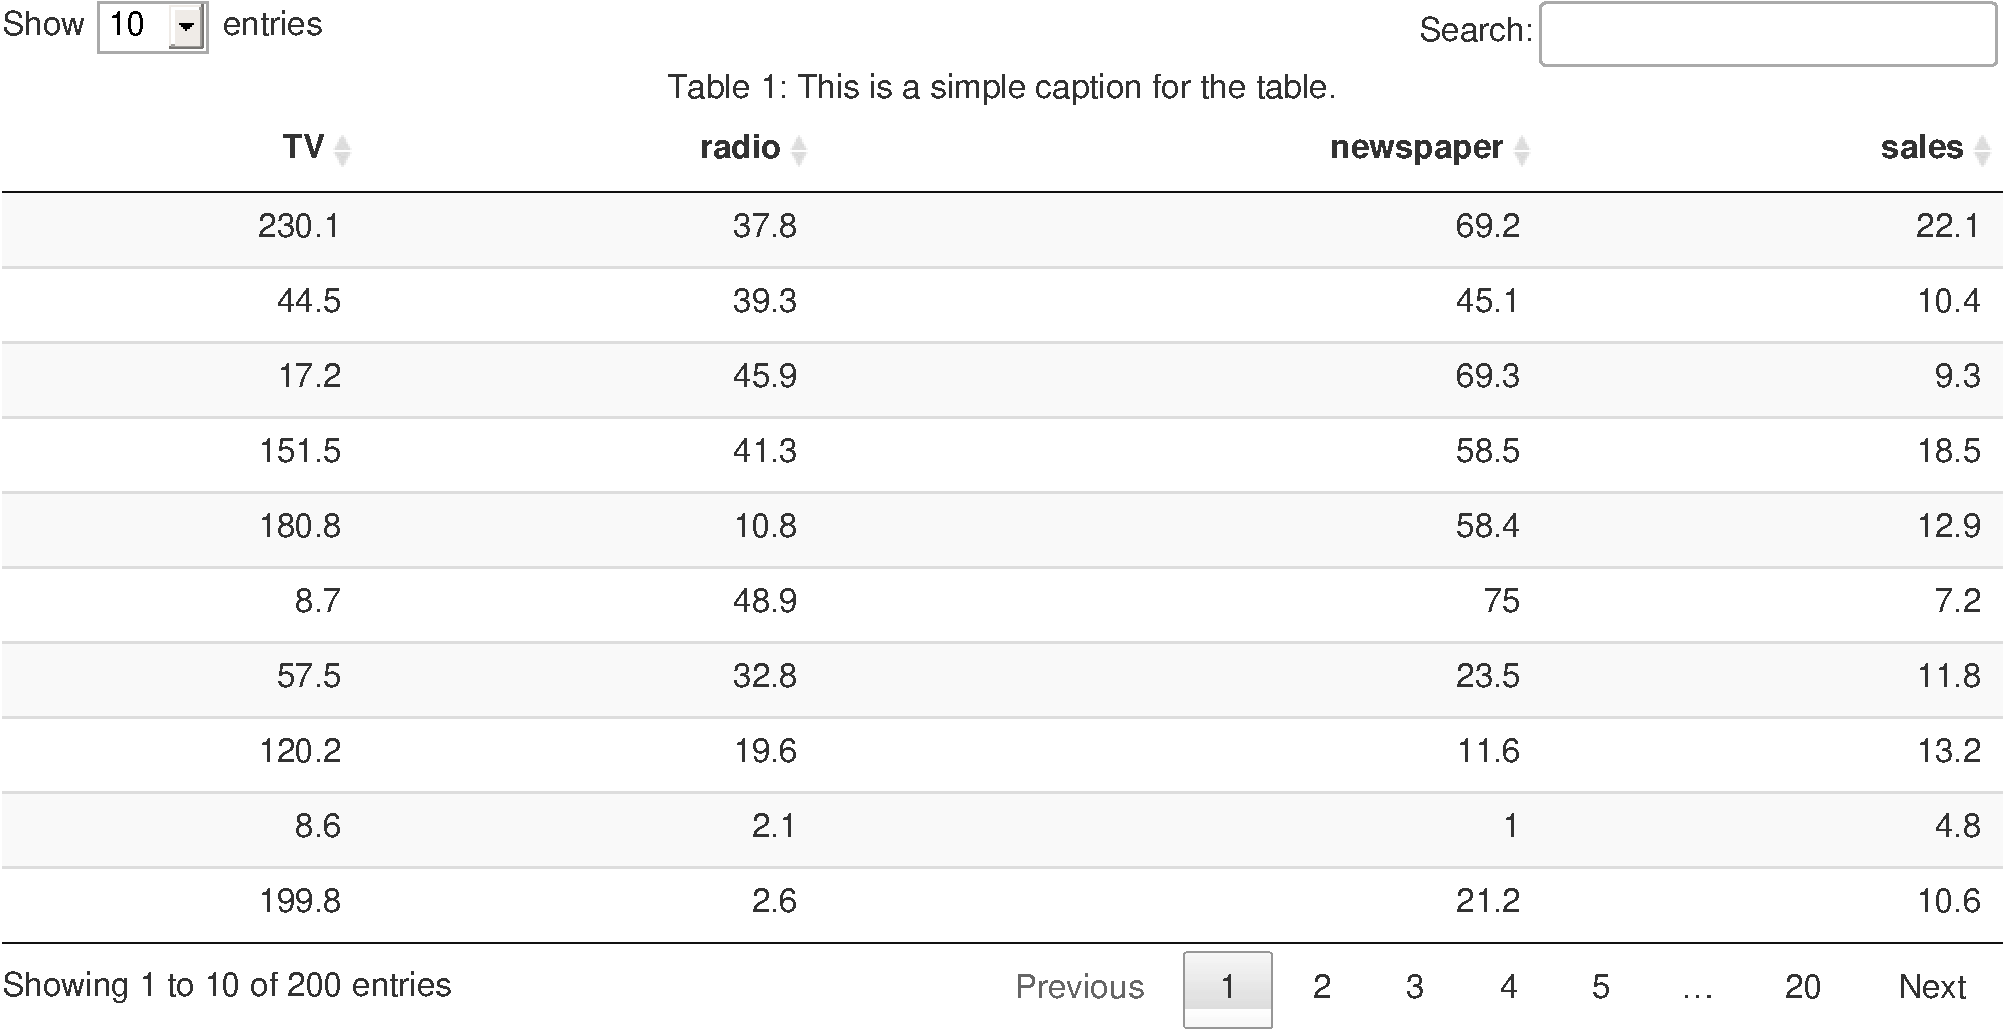
\includegraphics{SDM-CHAP24_files/figure-latex/readin-1} \end{center}

\hypertarget{base-r-graph}{%
\subsection{Base R Graph}\label{base-r-graph}}

\begin{Shaded}
\begin{Highlighting}[]
\FunctionTok{plot}\NormalTok{(sales }\SpecialCharTok{\textasciitilde{}}\NormalTok{ TV, }\AttributeTok{data =}\NormalTok{ AD, }\AttributeTok{col =} \StringTok{"red"}\NormalTok{, }\AttributeTok{pch =} \DecValTok{19}\NormalTok{)}
\NormalTok{mod1 }\OtherTok{\textless{}{-}} \FunctionTok{lm}\NormalTok{(sales }\SpecialCharTok{\textasciitilde{}}\NormalTok{ TV, }\AttributeTok{data =}\NormalTok{ AD)}
\FunctionTok{abline}\NormalTok{(mod1, }\AttributeTok{col =} \StringTok{"blue"}\NormalTok{)}
\end{Highlighting}
\end{Shaded}

\begin{figure}

{\centering 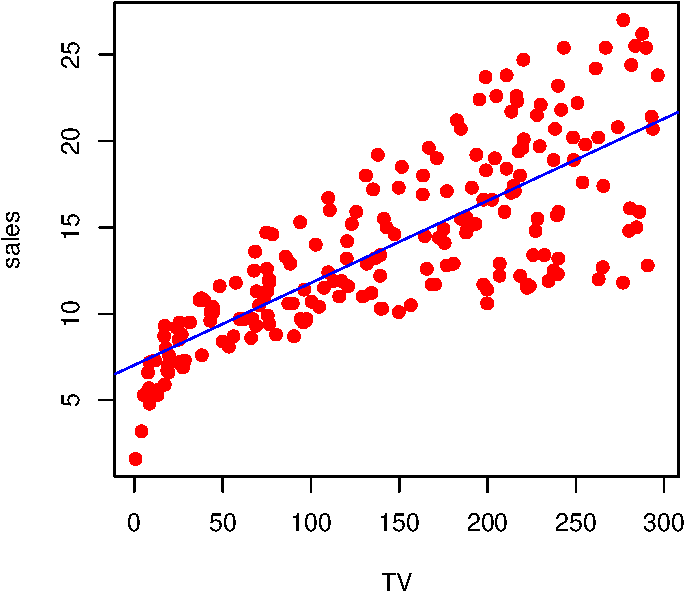
\includegraphics{SDM-CHAP24_files/figure-latex/base1-1} 

}

\caption{Base R scatterplot of `sales` versus `TV`}\label{fig:base1}
\end{figure}

\begin{Shaded}
\begin{Highlighting}[]
\FunctionTok{par}\NormalTok{(}\AttributeTok{mfrow =} \FunctionTok{c}\NormalTok{(}\DecValTok{1}\NormalTok{, }\DecValTok{3}\NormalTok{))}
\FunctionTok{plot}\NormalTok{(sales }\SpecialCharTok{\textasciitilde{}}\NormalTok{ TV, }\AttributeTok{data =}\NormalTok{ AD, }\AttributeTok{col =} \StringTok{"red"}\NormalTok{, }\AttributeTok{pch =} \DecValTok{19}\NormalTok{)}
\NormalTok{mod1 }\OtherTok{\textless{}{-}} \FunctionTok{lm}\NormalTok{(sales }\SpecialCharTok{\textasciitilde{}}\NormalTok{ TV, }\AttributeTok{data =}\NormalTok{ AD)}
\FunctionTok{abline}\NormalTok{(mod1, }\AttributeTok{col =} \StringTok{"blue"}\NormalTok{)}
\FunctionTok{plot}\NormalTok{(sales }\SpecialCharTok{\textasciitilde{}}\NormalTok{ radio, }\AttributeTok{data =}\NormalTok{ AD, }\AttributeTok{col =} \StringTok{"red"}\NormalTok{, }\AttributeTok{pch =} \DecValTok{19}\NormalTok{)}
\NormalTok{mod2 }\OtherTok{\textless{}{-}} \FunctionTok{lm}\NormalTok{(sales }\SpecialCharTok{\textasciitilde{}}\NormalTok{ radio, }\AttributeTok{data =}\NormalTok{ AD)}
\FunctionTok{abline}\NormalTok{(mod2, }\AttributeTok{col =} \StringTok{"blue"}\NormalTok{)}
\FunctionTok{plot}\NormalTok{(sales }\SpecialCharTok{\textasciitilde{}}\NormalTok{ newspaper, }\AttributeTok{data =}\NormalTok{ AD, }\AttributeTok{col =} \StringTok{"red"}\NormalTok{, }\AttributeTok{pch =} \DecValTok{19}\NormalTok{)}
\NormalTok{mod3 }\OtherTok{\textless{}{-}} \FunctionTok{lm}\NormalTok{(sales }\SpecialCharTok{\textasciitilde{}}\NormalTok{ newspaper, }\AttributeTok{data =}\NormalTok{ AD)}
\FunctionTok{abline}\NormalTok{(mod3, }\AttributeTok{col =} \StringTok{"blue"}\NormalTok{)}
\end{Highlighting}
\end{Shaded}

\begin{figure}

{\centering 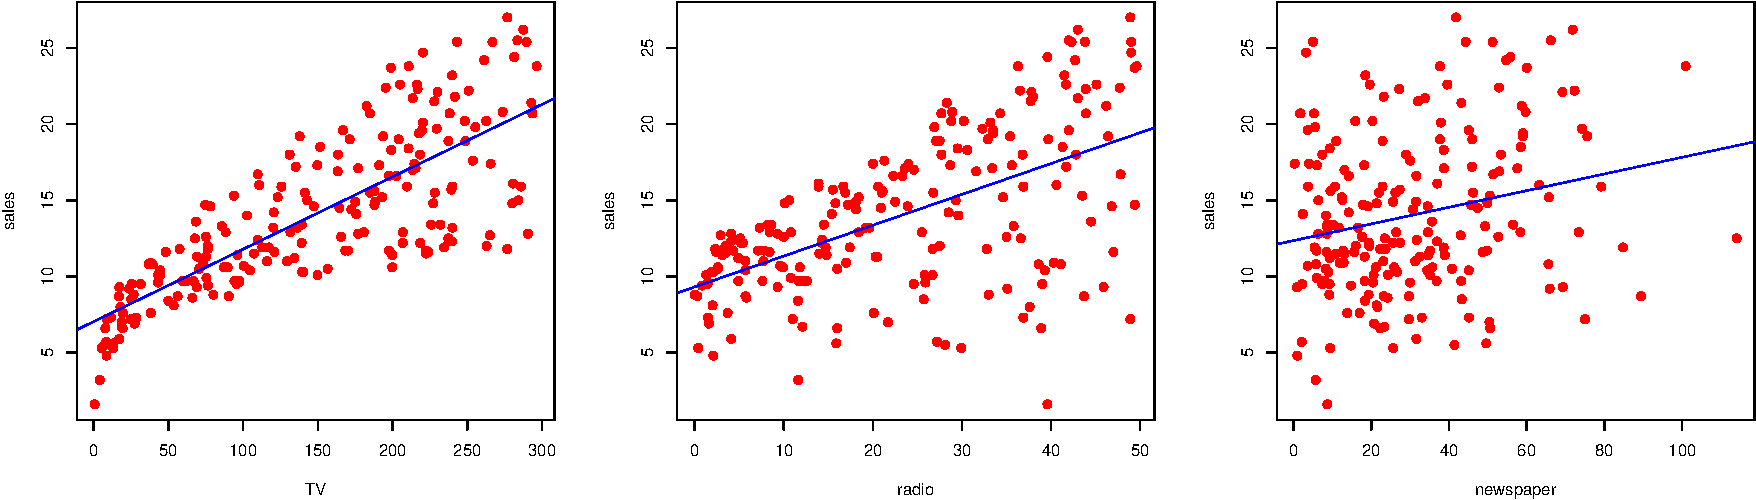
\includegraphics{SDM-CHAP24_files/figure-latex/youchange-1} 

}

\caption{You should change this caption}\label{fig:youchange}
\end{figure}

\begin{Shaded}
\begin{Highlighting}[]
\FunctionTok{par}\NormalTok{(}\AttributeTok{mfrow=}\FunctionTok{c}\NormalTok{(}\DecValTok{1}\NormalTok{, }\DecValTok{1}\NormalTok{))}
\end{Highlighting}
\end{Shaded}

Change the caption in Figure \ref{fig:youchange}.

\hypertarget{using-ggplot2}{%
\subsection{\texorpdfstring{Using \texttt{ggplot2}}{Using ggplot2}}\label{using-ggplot2}}

\begin{Shaded}
\begin{Highlighting}[]
\FunctionTok{library}\NormalTok{(ggplot2)}
\FunctionTok{library}\NormalTok{(MASS)}
\NormalTok{p }\OtherTok{\textless{}{-}} \FunctionTok{ggplot}\NormalTok{(}\AttributeTok{data =}\NormalTok{ AD, }\FunctionTok{aes}\NormalTok{(}\AttributeTok{x =}\NormalTok{ TV, }\AttributeTok{y =}\NormalTok{ sales)) }\SpecialCharTok{+}
  \FunctionTok{geom\_point}\NormalTok{(}\AttributeTok{color =} \StringTok{"lightblue"}\NormalTok{) }\SpecialCharTok{+}
  \FunctionTok{geom\_smooth}\NormalTok{(}\AttributeTok{method =} \StringTok{"lm"}\NormalTok{, }\AttributeTok{se =} \ConstantTok{FALSE}\NormalTok{, }\AttributeTok{color =} \StringTok{"blue"}\NormalTok{) }\SpecialCharTok{+}
  \FunctionTok{geom\_smooth}\NormalTok{(}\AttributeTok{method =} \StringTok{"loess"}\NormalTok{, }\AttributeTok{color =} \StringTok{"red"}\NormalTok{, }\AttributeTok{se =} \ConstantTok{FALSE}\NormalTok{) }\SpecialCharTok{+} 
  \FunctionTok{geom\_smooth}\NormalTok{(}\AttributeTok{method =} \StringTok{"rlm"}\NormalTok{, }\AttributeTok{color =} \StringTok{"purple"}\NormalTok{, }\AttributeTok{se =} \ConstantTok{FALSE}\NormalTok{) }\SpecialCharTok{+}
  \FunctionTok{theme\_bw}\NormalTok{()}
\NormalTok{p}
\end{Highlighting}
\end{Shaded}

\begin{center}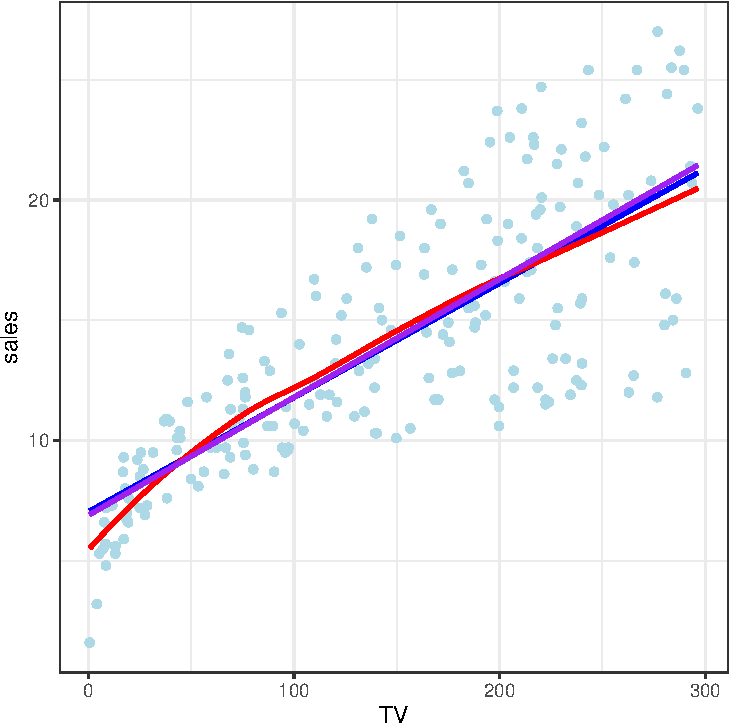
\includegraphics{SDM-CHAP24_files/figure-latex/ggp-1} \end{center}

\begin{Shaded}
\begin{Highlighting}[]
\FunctionTok{library}\NormalTok{(gridExtra)}
\NormalTok{p1 }\OtherTok{\textless{}{-}} \FunctionTok{ggplot}\NormalTok{(}\AttributeTok{data =}\NormalTok{ AD, }\FunctionTok{aes}\NormalTok{(}\AttributeTok{x =}\NormalTok{ TV, }\AttributeTok{y =}\NormalTok{ sales)) }\SpecialCharTok{+}
        \FunctionTok{geom\_point}\NormalTok{(}\AttributeTok{color =} \StringTok{"lightblue"}\NormalTok{) }\SpecialCharTok{+} 
        \FunctionTok{geom\_smooth}\NormalTok{(}\AttributeTok{method =} \StringTok{"lm"}\NormalTok{, }\AttributeTok{se =} \ConstantTok{FALSE}\NormalTok{, }\AttributeTok{color =} \StringTok{"blue"}\NormalTok{) }\SpecialCharTok{+}
        \FunctionTok{theme\_bw}\NormalTok{()}
\NormalTok{p2 }\OtherTok{\textless{}{-}} \FunctionTok{ggplot}\NormalTok{(}\AttributeTok{data =}\NormalTok{ AD, }\FunctionTok{aes}\NormalTok{(}\AttributeTok{x =}\NormalTok{ radio, }\AttributeTok{y =}\NormalTok{ sales)) }\SpecialCharTok{+}
        \FunctionTok{geom\_point}\NormalTok{(}\AttributeTok{color =} \StringTok{"lightblue"}\NormalTok{) }\SpecialCharTok{+}
        \FunctionTok{geom\_smooth}\NormalTok{(}\AttributeTok{method =} \StringTok{"lm"}\NormalTok{, }\AttributeTok{se =} \ConstantTok{FALSE}\NormalTok{, }\AttributeTok{color =} \StringTok{"blue"}\NormalTok{) }\SpecialCharTok{+}
        \FunctionTok{theme\_bw}\NormalTok{()}
\NormalTok{p3 }\OtherTok{\textless{}{-}} \FunctionTok{ggplot}\NormalTok{(}\AttributeTok{data =}\NormalTok{ AD, }\FunctionTok{aes}\NormalTok{(}\AttributeTok{x =}\NormalTok{ newspaper, }\AttributeTok{y =}\NormalTok{ sales)) }\SpecialCharTok{+}
        \FunctionTok{geom\_point}\NormalTok{(}\AttributeTok{color =} \StringTok{"lightblue"}\NormalTok{) }\SpecialCharTok{+}
        \FunctionTok{geom\_smooth}\NormalTok{(}\AttributeTok{method =} \StringTok{"lm"}\NormalTok{, }\AttributeTok{se =} \ConstantTok{FALSE}\NormalTok{, }\AttributeTok{color =} \StringTok{"blue"}\NormalTok{) }\SpecialCharTok{+} 
        \FunctionTok{theme\_bw}\NormalTok{()}
\FunctionTok{grid.arrange}\NormalTok{(p1, p2, p3, }\AttributeTok{ncol =} \DecValTok{3}\NormalTok{)}
\end{Highlighting}
\end{Shaded}

\begin{figure}

{\centering 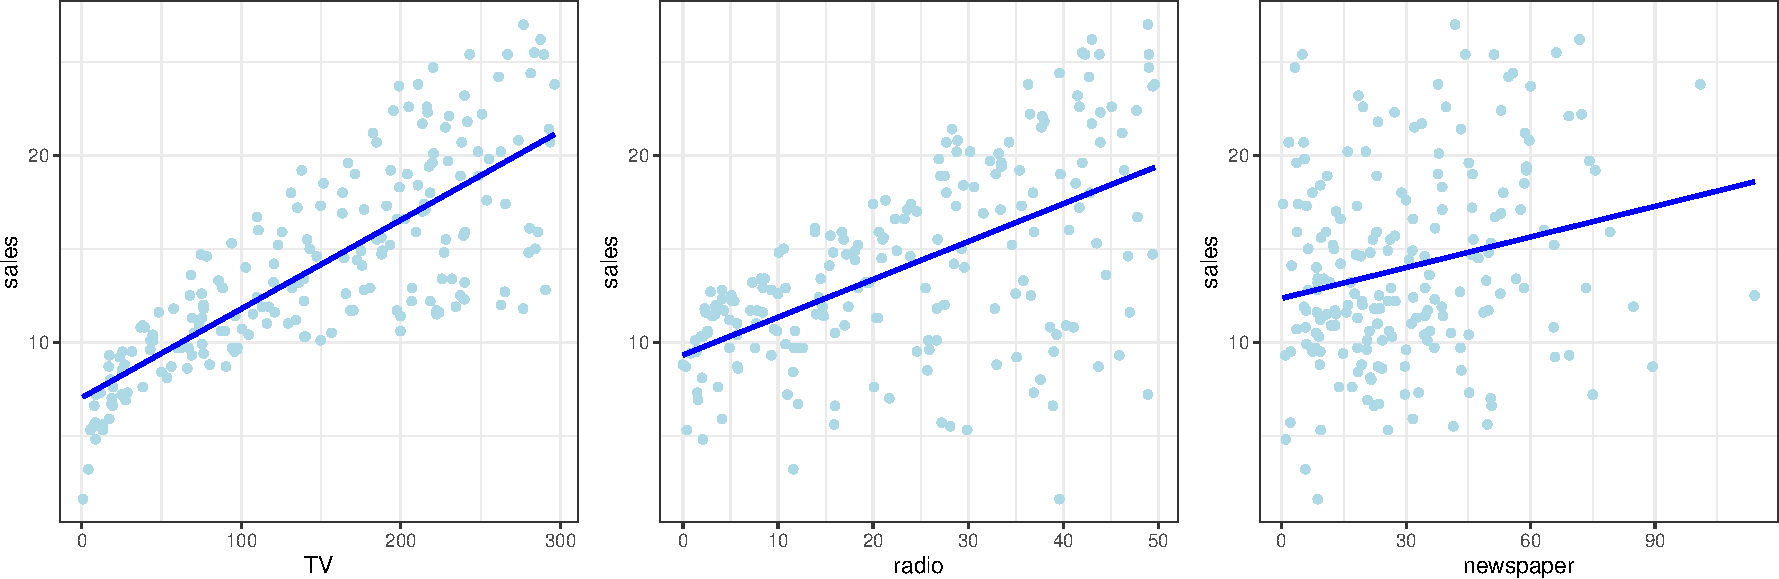
\includegraphics{SDM-CHAP24_files/figure-latex/unnamed-chunk-1-1} 

}

\caption{Using `grid.arrange()` with `ggplot`}\label{fig:unnamed-chunk-1}
\end{figure}

\hypertarget{using-plotly}{%
\subsection{\texorpdfstring{Using \texttt{plotly}}{Using plotly}}\label{using-plotly}}

First create a plot with \texttt{ggplot2}, then pass the \texttt{ggplot2} object to \texttt{ggplotly} from the \texttt{plotly} package.

\begin{Shaded}
\begin{Highlighting}[]
\FunctionTok{library}\NormalTok{(plotly)}
\NormalTok{p11 }\OtherTok{\textless{}{-}} \FunctionTok{ggplotly}\NormalTok{(p)}
\NormalTok{p11}
\end{Highlighting}
\end{Shaded}

\begin{center}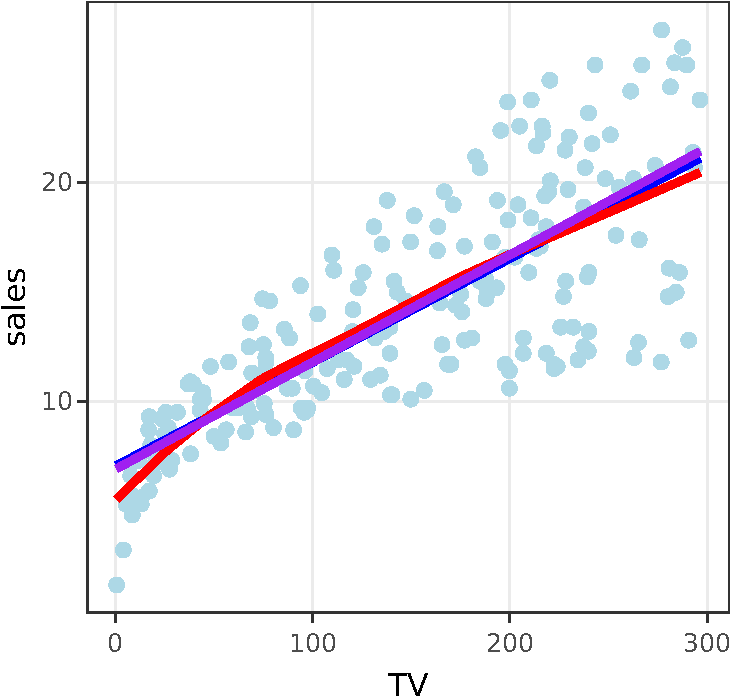
\includegraphics{SDM-CHAP24_files/figure-latex/plotly-1} \end{center}

\hypertarget{scatterplot-matrices}{%
\subsection{Scatterplot Matrices}\label{scatterplot-matrices}}

\begin{Shaded}
\begin{Highlighting}[]
\FunctionTok{library}\NormalTok{(car)}
\FunctionTok{scatterplotMatrix}\NormalTok{(}\SpecialCharTok{\textasciitilde{}}\NormalTok{ sales }\SpecialCharTok{+}\NormalTok{ TV }\SpecialCharTok{+}\NormalTok{ radio }\SpecialCharTok{+}\NormalTok{ newspaper, }\AttributeTok{data =}\NormalTok{ AD)}
\end{Highlighting}
\end{Shaded}

\begin{center}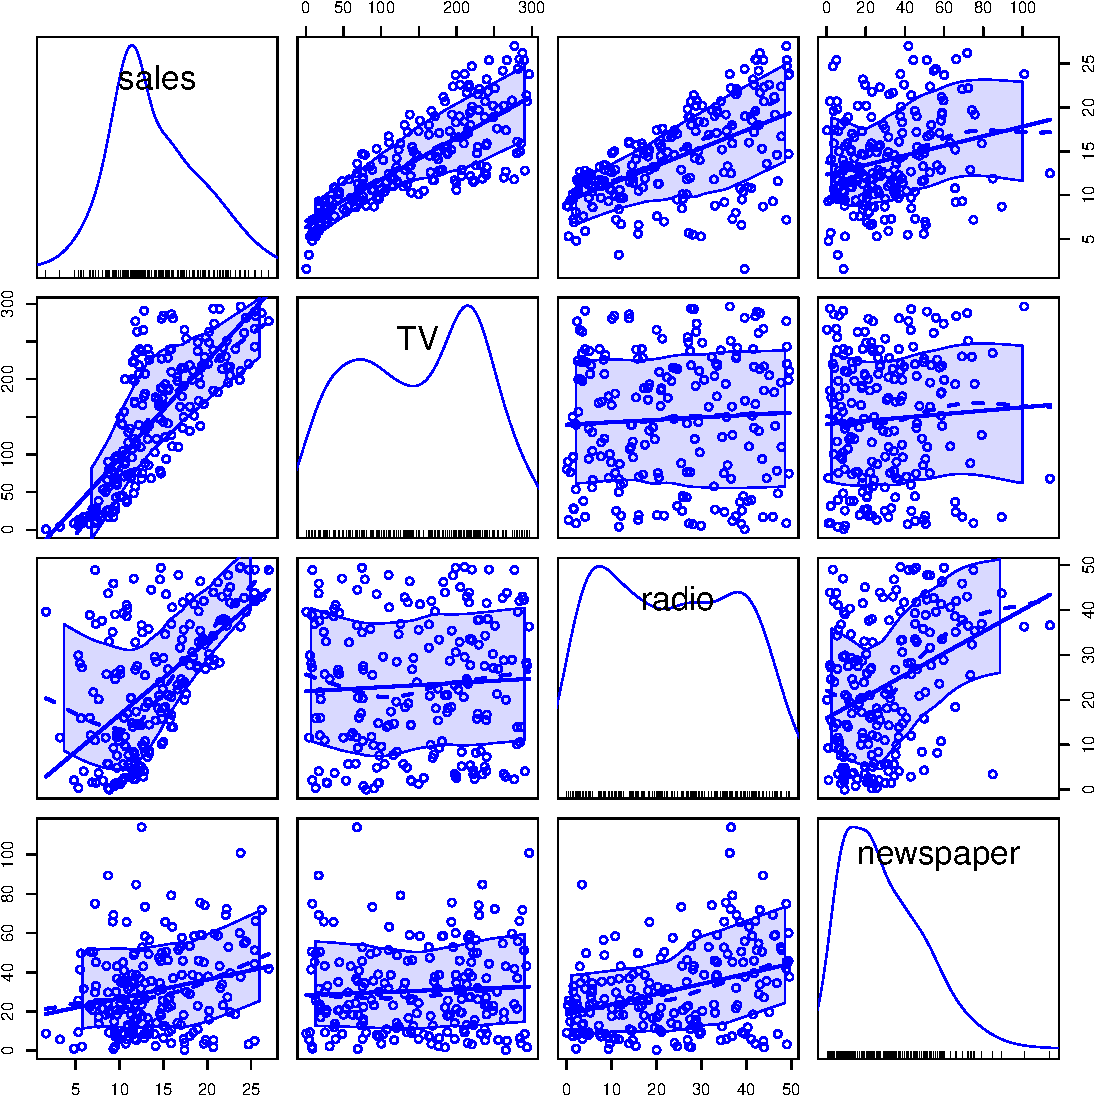
\includegraphics{SDM-CHAP24_files/figure-latex/SPM-1} \end{center}

\hypertarget{basic-regression}{%
\section{Basic Regression}\label{basic-regression}}

Recall \texttt{mod1}

\begin{Shaded}
\begin{Highlighting}[]
\NormalTok{mod1 }\OtherTok{\textless{}{-}} \FunctionTok{lm}\NormalTok{(sales }\SpecialCharTok{\textasciitilde{}}\NormalTok{ TV, }\AttributeTok{data =}\NormalTok{ AD)}
\FunctionTok{summary}\NormalTok{(mod1)}
\end{Highlighting}
\end{Shaded}

\begin{verbatim}
Call:
lm(formula = sales ~ TV, data = AD)

Residuals:
    Min      1Q  Median      3Q     Max 
-8.3860 -1.9545 -0.1913  2.0671  7.2124 

Coefficients:
            Estimate Std. Error t value Pr(>|t|)    
(Intercept) 7.032594   0.457843   15.36   <2e-16 ***
TV          0.047537   0.002691   17.67   <2e-16 ***
---
Signif. codes:  0 '***' 0.001 '**' 0.01 '*' 0.05 '.' 0.1 ' ' 1

Residual standard error: 3.259 on 198 degrees of freedom
Multiple R-squared:  0.6119,    Adjusted R-squared:  0.6099 
F-statistic: 312.1 on 1 and 198 DF,  p-value: < 2.2e-16
\end{verbatim}

\begin{equation}
\text{Residual}\equiv e_i = y_i - \hat{y_i}
\label{eq:resid}
\end{equation}

To obtain the residuals for \texttt{mod1} use the function \texttt{resid} on a linear model object.

\begin{Shaded}
\begin{Highlighting}[]
\NormalTok{eis }\OtherTok{\textless{}{-}} \FunctionTok{resid}\NormalTok{(mod1)}
\NormalTok{RSS }\OtherTok{\textless{}{-}} \FunctionTok{sum}\NormalTok{(eis}\SpecialCharTok{\^{}}\DecValTok{2}\NormalTok{)}
\NormalTok{RSS}
\end{Highlighting}
\end{Shaded}

\begin{verbatim}
[1] 2102.531
\end{verbatim}

\begin{Shaded}
\begin{Highlighting}[]
\NormalTok{RSE }\OtherTok{\textless{}{-}} \FunctionTok{sqrt}\NormalTok{(RSS}\SpecialCharTok{/}\NormalTok{(}\FunctionTok{dim}\NormalTok{(AD)[}\DecValTok{1}\NormalTok{]}\SpecialCharTok{{-}}\DecValTok{2}\NormalTok{))}
\NormalTok{RSE}
\end{Highlighting}
\end{Shaded}

\begin{verbatim}
[1] 3.258656
\end{verbatim}

\begin{Shaded}
\begin{Highlighting}[]
\CommentTok{\# Or}
\FunctionTok{summary}\NormalTok{(mod1)}\SpecialCharTok{$}\NormalTok{sigma}
\end{Highlighting}
\end{Shaded}

\begin{verbatim}
[1] 3.258656
\end{verbatim}

\begin{Shaded}
\begin{Highlighting}[]
\CommentTok{\# Or}
\FunctionTok{library}\NormalTok{(broom)}
\NormalTok{NDF }\OtherTok{\textless{}{-}} \FunctionTok{augment}\NormalTok{(mod1)}
\FunctionTok{sum}\NormalTok{(NDF}\SpecialCharTok{$}\NormalTok{.resid}\SpecialCharTok{\^{}}\DecValTok{2}\NormalTok{)}
\end{Highlighting}
\end{Shaded}

\begin{verbatim}
[1] 2102.531
\end{verbatim}

\begin{Shaded}
\begin{Highlighting}[]
\NormalTok{RSE }\OtherTok{\textless{}{-}} \FunctionTok{sqrt}\NormalTok{(}\FunctionTok{sum}\NormalTok{(NDF}\SpecialCharTok{$}\NormalTok{.resid}\SpecialCharTok{\^{}}\DecValTok{2}\NormalTok{)}\SpecialCharTok{/}\FunctionTok{df.residual}\NormalTok{(mod1))}
\NormalTok{RSE}
\end{Highlighting}
\end{Shaded}

\begin{verbatim}
[1] 3.258656
\end{verbatim}

\begin{Shaded}
\begin{Highlighting}[]
\FunctionTok{library}\NormalTok{(moderndive)}
\FunctionTok{get\_regression\_table}\NormalTok{(mod1)}
\end{Highlighting}
\end{Shaded}

\begin{verbatim}
# A tibble: 2 x 7
  term      estimate std_error statistic p_value lower_ci upper_ci
  <chr>        <dbl>     <dbl>     <dbl>   <dbl>    <dbl>    <dbl>
1 intercept    7.03      0.458      15.4       0    6.13     7.94 
2 TV           0.048     0.003      17.7       0    0.042    0.053
\end{verbatim}

\begin{Shaded}
\begin{Highlighting}[]
\NormalTok{MDDF }\OtherTok{\textless{}{-}} \FunctionTok{get\_regression\_points}\NormalTok{(mod1)}
\NormalTok{MDDF}
\end{Highlighting}
\end{Shaded}

\begin{verbatim}
# A tibble: 200 x 5
      ID sales    TV sales_hat residual
   <int> <dbl> <dbl>     <dbl>    <dbl>
 1     1  22.1 230.      18.0     4.13 
 2     2  10.4  44.5      9.15    1.25 
 3     3   9.3  17.2      7.85    1.45 
 4     4  18.5 152.      14.2     4.27 
 5     5  12.9 181.      15.6    -2.73 
 6     6   7.2   8.7      7.45   -0.246
 7     7  11.8  57.5      9.77    2.03 
 8     8  13.2 120.      12.7     0.454
 9     9   4.8   8.6      7.44   -2.64 
10    10  10.6 200.      16.5    -5.93 
# ... with 190 more rows
\end{verbatim}

\begin{Shaded}
\begin{Highlighting}[]
\FunctionTok{library}\NormalTok{(dplyr)}
\NormalTok{MDDF }\SpecialCharTok{\%\textgreater{}\%} 
  \FunctionTok{summarize}\NormalTok{(}\AttributeTok{RSS =} \FunctionTok{sum}\NormalTok{(residual}\SpecialCharTok{\^{}}\DecValTok{2}\NormalTok{))}
\end{Highlighting}
\end{Shaded}

\begin{verbatim}
# A tibble: 1 x 1
    RSS
  <dbl>
1 2102.
\end{verbatim}

The least squares estimators of \(\beta_0\) and \(\beta_1\) are

\[b_0 = \hat{\beta_0} = \bar{y} - b_1\bar{x}\]
\[b_1 = \hat{\beta_1} = \frac{\sum_{i = 1}^n(x_i - \bar{x})(y_i - \bar{y})}{\sum_{i=1}^n(x_i-\bar{x})^2}\]

\begin{Shaded}
\begin{Highlighting}[]
\NormalTok{y }\OtherTok{\textless{}{-}}\NormalTok{ AD}\SpecialCharTok{$}\NormalTok{sales}
\NormalTok{x }\OtherTok{\textless{}{-}}\NormalTok{ AD}\SpecialCharTok{$}\NormalTok{TV}
\NormalTok{b1 }\OtherTok{\textless{}{-}} \FunctionTok{sum}\NormalTok{( (x }\SpecialCharTok{{-}} \FunctionTok{mean}\NormalTok{(x))}\SpecialCharTok{*}\NormalTok{(y }\SpecialCharTok{{-}} \FunctionTok{mean}\NormalTok{(y)) ) }\SpecialCharTok{/} \FunctionTok{sum}\NormalTok{((x }\SpecialCharTok{{-}} \FunctionTok{mean}\NormalTok{(x))}\SpecialCharTok{\^{}}\DecValTok{2}\NormalTok{)}
\NormalTok{b0 }\OtherTok{\textless{}{-}} \FunctionTok{mean}\NormalTok{(y) }\SpecialCharTok{{-}}\NormalTok{ b1}\SpecialCharTok{*}\FunctionTok{mean}\NormalTok{(x)}
\FunctionTok{c}\NormalTok{(b0, b1)}
\end{Highlighting}
\end{Shaded}

\begin{verbatim}
[1] 7.03259355 0.04753664
\end{verbatim}

\begin{Shaded}
\begin{Highlighting}[]
\CommentTok{\# Or using}
\FunctionTok{coef}\NormalTok{(mod1)}
\end{Highlighting}
\end{Shaded}

\begin{verbatim}
(Intercept)          TV 
 7.03259355  0.04753664 
\end{verbatim}

\begin{Shaded}
\begin{Highlighting}[]
\FunctionTok{summary}\NormalTok{(mod1)}
\end{Highlighting}
\end{Shaded}

\begin{verbatim}
Call:
lm(formula = sales ~ TV, data = AD)

Residuals:
    Min      1Q  Median      3Q     Max 
-8.3860 -1.9545 -0.1913  2.0671  7.2124 

Coefficients:
            Estimate Std. Error t value Pr(>|t|)    
(Intercept) 7.032594   0.457843   15.36   <2e-16 ***
TV          0.047537   0.002691   17.67   <2e-16 ***
---
Signif. codes:  0 '***' 0.001 '**' 0.01 '*' 0.05 '.' 0.1 ' ' 1

Residual standard error: 3.259 on 198 degrees of freedom
Multiple R-squared:  0.6119,    Adjusted R-squared:  0.6099 
F-statistic: 312.1 on 1 and 198 DF,  p-value: < 2.2e-16
\end{verbatim}

\begin{Shaded}
\begin{Highlighting}[]
\NormalTok{XTXI }\OtherTok{\textless{}{-}} \FunctionTok{summary}\NormalTok{(mod1)}\SpecialCharTok{$}\NormalTok{cov.unscaled}
\NormalTok{MSE }\OtherTok{\textless{}{-}} \FunctionTok{summary}\NormalTok{(mod1)}\SpecialCharTok{$}\NormalTok{sigma}\SpecialCharTok{\^{}}\DecValTok{2}
\NormalTok{var.cov.b }\OtherTok{\textless{}{-}}\NormalTok{ MSE}\SpecialCharTok{*}\NormalTok{XTXI}
\NormalTok{var.cov.b}
\end{Highlighting}
\end{Shaded}

\begin{verbatim}
             (Intercept)            TV
(Intercept)  0.209620158 -1.064495e-03
TV          -0.001064495  7.239367e-06
\end{verbatim}

\begin{Shaded}
\begin{Highlighting}[]
\NormalTok{seb0 }\OtherTok{\textless{}{-}} \FunctionTok{sqrt}\NormalTok{(var.cov.b[}\DecValTok{1}\NormalTok{, }\DecValTok{1}\NormalTok{])}
\NormalTok{seb1 }\OtherTok{\textless{}{-}} \FunctionTok{sqrt}\NormalTok{(var.cov.b[}\DecValTok{2}\NormalTok{, }\DecValTok{2}\NormalTok{])}
\FunctionTok{c}\NormalTok{(seb0, seb1)}
\end{Highlighting}
\end{Shaded}

\begin{verbatim}
[1] 0.457842940 0.002690607
\end{verbatim}

\begin{Shaded}
\begin{Highlighting}[]
\FunctionTok{coef}\NormalTok{(}\FunctionTok{summary}\NormalTok{(mod1))}
\end{Highlighting}
\end{Shaded}

\begin{verbatim}
              Estimate  Std. Error  t value    Pr(>|t|)
(Intercept) 7.03259355 0.457842940 15.36028 1.40630e-35
TV          0.04753664 0.002690607 17.66763 1.46739e-42
\end{verbatim}

\begin{Shaded}
\begin{Highlighting}[]
\FunctionTok{coef}\NormalTok{(}\FunctionTok{summary}\NormalTok{(mod1))[}\DecValTok{1}\NormalTok{, }\DecValTok{2}\NormalTok{]}
\end{Highlighting}
\end{Shaded}

\begin{verbatim}
[1] 0.4578429
\end{verbatim}

\begin{Shaded}
\begin{Highlighting}[]
\FunctionTok{coef}\NormalTok{(}\FunctionTok{summary}\NormalTok{(mod1))[}\DecValTok{2}\NormalTok{, }\DecValTok{2}\NormalTok{]}
\end{Highlighting}
\end{Shaded}

\begin{verbatim}
[1] 0.002690607
\end{verbatim}

\begin{Shaded}
\begin{Highlighting}[]
\NormalTok{tb0 }\OtherTok{\textless{}{-}}\NormalTok{ b0}\SpecialCharTok{/}\NormalTok{seb0}
\NormalTok{tb1 }\OtherTok{\textless{}{-}}\NormalTok{ b1}\SpecialCharTok{/}\NormalTok{seb1}
\FunctionTok{c}\NormalTok{(tb0, tb1)}
\end{Highlighting}
\end{Shaded}

\begin{verbatim}
[1] 15.36028 17.66763
\end{verbatim}

\begin{Shaded}
\begin{Highlighting}[]
\NormalTok{pvalues }\OtherTok{\textless{}{-}} \FunctionTok{c}\NormalTok{(}\FunctionTok{pt}\NormalTok{(tb0, }\DecValTok{198}\NormalTok{, }\AttributeTok{lower =} \ConstantTok{FALSE}\NormalTok{)}\SpecialCharTok{*}\DecValTok{2}\NormalTok{, }\FunctionTok{pt}\NormalTok{(tb1, }\DecValTok{198}\NormalTok{, }\AttributeTok{lower =} \ConstantTok{FALSE}\NormalTok{)}\SpecialCharTok{*}\DecValTok{2}\NormalTok{)}
\NormalTok{pvalues}
\end{Highlighting}
\end{Shaded}

\begin{verbatim}
[1] 1.40630e-35 1.46739e-42
\end{verbatim}

\begin{Shaded}
\begin{Highlighting}[]
\FunctionTok{coef}\NormalTok{(}\FunctionTok{summary}\NormalTok{(mod1))}
\end{Highlighting}
\end{Shaded}

\begin{verbatim}
              Estimate  Std. Error  t value    Pr(>|t|)
(Intercept) 7.03259355 0.457842940 15.36028 1.40630e-35
TV          0.04753664 0.002690607 17.66763 1.46739e-42
\end{verbatim}

\begin{Shaded}
\begin{Highlighting}[]
\NormalTok{TSS }\OtherTok{\textless{}{-}} \FunctionTok{sum}\NormalTok{((y }\SpecialCharTok{{-}} \FunctionTok{mean}\NormalTok{(y))}\SpecialCharTok{\^{}}\DecValTok{2}\NormalTok{)}
\FunctionTok{c}\NormalTok{(RSS, TSS)}
\end{Highlighting}
\end{Shaded}

\begin{verbatim}
[1] 2102.531 5417.149
\end{verbatim}

\begin{Shaded}
\begin{Highlighting}[]
\NormalTok{R2 }\OtherTok{\textless{}{-}}\NormalTok{ (TSS }\SpecialCharTok{{-}}\NormalTok{ RSS)}\SpecialCharTok{/}\NormalTok{TSS}
\NormalTok{R2}
\end{Highlighting}
\end{Shaded}

\begin{verbatim}
[1] 0.6118751
\end{verbatim}

\begin{Shaded}
\begin{Highlighting}[]
\CommentTok{\# Or}
\FunctionTok{summary}\NormalTok{(mod1)}\SpecialCharTok{$}\NormalTok{r.squared}
\end{Highlighting}
\end{Shaded}

\begin{verbatim}
[1] 0.6118751
\end{verbatim}

\hypertarget{confidence-interval-for-beta_1}{%
\subsection{\texorpdfstring{Confidence Interval for \(\beta_1\)}{Confidence Interval for \textbackslash beta\_1}}\label{confidence-interval-for-beta_1}}

\begin{equation}
\text{CI}_{1 - \alpha}(\beta_1) = \left[b_1 - t_{1- \alpha/2, n - p + 1}SE(b1), b_1 + t_{1- \alpha/2, n - p + 1}SE(b1) \right]
\label{eq:ci}
\end{equation}

\textbf{Example:} Use Equation \eqref{eq:ci} to construct a 90\% confidence interval for \(\beta_1\).

\begin{Shaded}
\begin{Highlighting}[]
\NormalTok{alpha }\OtherTok{\textless{}{-}} \FloatTok{0.10}
\NormalTok{ct }\OtherTok{\textless{}{-}} \FunctionTok{qt}\NormalTok{(}\DecValTok{1} \SpecialCharTok{{-}}\NormalTok{ alpha}\SpecialCharTok{/}\DecValTok{2}\NormalTok{, }\FunctionTok{df.residual}\NormalTok{(mod1))}
\NormalTok{ct}
\end{Highlighting}
\end{Shaded}

\begin{verbatim}
[1] 1.652586
\end{verbatim}

\begin{Shaded}
\begin{Highlighting}[]
\NormalTok{b1 }\SpecialCharTok{+} \FunctionTok{c}\NormalTok{(}\SpecialCharTok{{-}}\DecValTok{1}\NormalTok{, }\DecValTok{1}\NormalTok{)}\SpecialCharTok{*}\NormalTok{ct}\SpecialCharTok{*}\NormalTok{seb1}
\end{Highlighting}
\end{Shaded}

\begin{verbatim}
[1] 0.04309018 0.05198310
\end{verbatim}

\begin{Shaded}
\begin{Highlighting}[]
\CommentTok{\# Or}
\FunctionTok{confint}\NormalTok{(mod1, }\AttributeTok{parm =} \StringTok{"TV"}\NormalTok{, }\AttributeTok{level =} \FloatTok{0.90}\NormalTok{)}
\end{Highlighting}
\end{Shaded}

\begin{verbatim}
          5 %      95 %
TV 0.04309018 0.0519831
\end{verbatim}

\begin{Shaded}
\begin{Highlighting}[]
\FunctionTok{confint}\NormalTok{(mod1)}
\end{Highlighting}
\end{Shaded}

\begin{verbatim}
                 2.5 %     97.5 %
(Intercept) 6.12971927 7.93546783
TV          0.04223072 0.05284256
\end{verbatim}

\hypertarget{linear-algebra}{%
\subsubsection{Linear Algebra}\label{linear-algebra}}

\textbf{Solution of linear systems} Find the solution(s) if any to the following linear equations.

\[2x + y - z = 8\]
\[-3x - y + 2z = -11\]
\[-2x + y + 2z = -3\]

\begin{Shaded}
\begin{Highlighting}[]
\NormalTok{A }\OtherTok{\textless{}{-}} \FunctionTok{matrix}\NormalTok{(}\FunctionTok{c}\NormalTok{(}\DecValTok{2}\NormalTok{, }\SpecialCharTok{{-}}\DecValTok{3}\NormalTok{, }\SpecialCharTok{{-}}\DecValTok{2}\NormalTok{, }\DecValTok{1}\NormalTok{, }\SpecialCharTok{{-}}\DecValTok{1}\NormalTok{, }\DecValTok{1}\NormalTok{, }\SpecialCharTok{{-}}\DecValTok{1}\NormalTok{, }\DecValTok{2}\NormalTok{, }\DecValTok{2}\NormalTok{), }\AttributeTok{nrow =} \DecValTok{3}\NormalTok{)}
\NormalTok{b }\OtherTok{\textless{}{-}} \FunctionTok{matrix}\NormalTok{(}\FunctionTok{c}\NormalTok{(}\DecValTok{8}\NormalTok{, }\SpecialCharTok{{-}}\DecValTok{11}\NormalTok{, }\SpecialCharTok{{-}}\DecValTok{3}\NormalTok{), }\AttributeTok{nrow =} \DecValTok{3}\NormalTok{)}
\NormalTok{x }\OtherTok{\textless{}{-}} \FunctionTok{solve}\NormalTok{(A)}\SpecialCharTok{\%*\%}\NormalTok{b}
\NormalTok{x}
\end{Highlighting}
\end{Shaded}

\begin{verbatim}
     [,1]
[1,]    2
[2,]    3
[3,]   -1
\end{verbatim}

\begin{Shaded}
\begin{Highlighting}[]
\CommentTok{\# Or}
\FunctionTok{solve}\NormalTok{(A, b)}
\end{Highlighting}
\end{Shaded}

\begin{verbatim}
     [,1]
[1,]    2
[2,]    3
[3,]   -1
\end{verbatim}

See \href{https://en.wikipedia.org/wiki/Matrix_multiplication}{wikipedia} for a review of matrix multiplication rules and properties.

Consider the 2 \(\times\) 2 matrix \(A\).

\[A = \begin{bmatrix}
2 & 4 \\
9 & 5 \\
\end{bmatrix}
\]

\hypertarget{linear-regression-matrix-notation}{%
\subsubsection{Linear Regression Matrix Notation}\label{linear-regression-matrix-notation}}

\begin{equation}
\hat{\mathbf{\beta}} = (\mathbf{X'X})^{-1}\mathbf{X'Y}
\label{eq:betas}
\end{equation}

\begin{equation}
\sigma^2_{\hat{\beta}} = \sigma^2(\mathbf{X'X})^{-1}
\label{eq:varcov}
\end{equation}

\begin{equation}
\hat{\sigma}^2_{\hat{\beta}} = MSE(\mathbf{X'X})^{-1}
\label{eq:varcovest}
\end{equation}

\[\hat{\mathbf{\beta}} \sim\mathcal{N}(\mathbf{\beta}, \sigma^2(\mathbf{X'X})^{-1})\]

\hypertarget{estimation-of-the-mean-response-for-new-values-x_h}{%
\subsubsection{\texorpdfstring{Estimation of the Mean Response for New Values \(X_h\)}{Estimation of the Mean Response for New Values X\_h}}\label{estimation-of-the-mean-response-for-new-values-x_h}}

Not only is it desirable to create confidence intervals on the parameters of the regression models, bit it is also common to estimate the mean response \(\left(E(Y_h)\right)\) for a particular set of \(\mathbf{X}\) values.

\[\hat{Y}_h \sim \mathcal{N}(Y_h = X_h\beta, \sigma^2\mathbf{X_h}(\mathbf{X'X})^{-1}\mathbf{X_h'})\]
For a vector of given values \((\mathbf{X_h})\), a \((1 - \alpha)\cdot 100\%\) confidence interval for the mean response \(E(Y_h)\) is

\[CI_{1-\alpha}\left[E(Y_h)\right] = \left[\hat{Y}_h - t_{1 - \alpha/2;n - p - 1}\cdot s_{\hat{Y}_h}, \hat{Y}_h + t_{1 - \alpha/2;n - p - 1}\cdot s_{\hat{Y}_h}  \right]\]
The function \texttt{predict()} applied to a linear model object will compute \(\hat{Y}_h\) and \(s_{\hat{Y}_h}\) for a given \(\mathbf{X}_h\). \texttt{R} output has \(\hat{Y}_h\) labeled \texttt{fit} and \(s_{\hat{Y}_h}\) labeled \texttt{se.fit}.

\begin{Shaded}
\begin{Highlighting}[]
\NormalTok{A }\OtherTok{\textless{}{-}} \FunctionTok{matrix}\NormalTok{(}\FunctionTok{c}\NormalTok{(}\DecValTok{2}\NormalTok{, }\DecValTok{9}\NormalTok{, }\DecValTok{4}\NormalTok{, }\DecValTok{5}\NormalTok{), }\AttributeTok{nrow =} \DecValTok{2}\NormalTok{)}
\NormalTok{A}
\end{Highlighting}
\end{Shaded}

\begin{verbatim}
     [,1] [,2]
[1,]    2    4
[2,]    9    5
\end{verbatim}

\begin{Shaded}
\begin{Highlighting}[]
\FunctionTok{t}\NormalTok{(A)          }\CommentTok{\# Transpose of A}
\end{Highlighting}
\end{Shaded}

\begin{verbatim}
     [,1] [,2]
[1,]    2    9
[2,]    4    5
\end{verbatim}

\begin{Shaded}
\begin{Highlighting}[]
\FunctionTok{t}\NormalTok{(A)}\SpecialCharTok{\%*\%}\NormalTok{A      }\CommentTok{\# A\textquotesingle{}A}
\end{Highlighting}
\end{Shaded}

\begin{verbatim}
     [,1] [,2]
[1,]   85   53
[2,]   53   41
\end{verbatim}

\begin{Shaded}
\begin{Highlighting}[]
\FunctionTok{solve}\NormalTok{(A)}\SpecialCharTok{\%*\%}\NormalTok{A  }\CommentTok{\# I\_2}
\end{Highlighting}
\end{Shaded}

\begin{verbatim}
             [,1]          [,2]
[1,] 1.000000e+00 -1.110223e-16
[2,] 1.110223e-16  1.000000e+00
\end{verbatim}

\begin{Shaded}
\begin{Highlighting}[]
\FunctionTok{zapsmall}\NormalTok{(}\FunctionTok{solve}\NormalTok{(A)}\SpecialCharTok{\%*\%}\NormalTok{A)  }\CommentTok{\# What you expect I\_2}
\end{Highlighting}
\end{Shaded}

\begin{verbatim}
     [,1] [,2]
[1,]    1    0
[2,]    0    1
\end{verbatim}

\begin{Shaded}
\begin{Highlighting}[]
\NormalTok{X }\OtherTok{\textless{}{-}} \FunctionTok{model.matrix}\NormalTok{(mod1)}
\NormalTok{XTX }\OtherTok{\textless{}{-}} \FunctionTok{t}\NormalTok{(X)}\SpecialCharTok{\%*\%}\NormalTok{X}
\FunctionTok{dim}\NormalTok{(XTX)}
\end{Highlighting}
\end{Shaded}

\begin{verbatim}
[1] 2 2
\end{verbatim}

\begin{Shaded}
\begin{Highlighting}[]
\NormalTok{XTXI }\OtherTok{\textless{}{-}} \FunctionTok{solve}\NormalTok{(XTX)}
\NormalTok{XTXI}
\end{Highlighting}
\end{Shaded}

\begin{verbatim}
              (Intercept)            TV
(Intercept)  0.0197403984 -1.002458e-04
TV          -0.0001002458  6.817474e-07
\end{verbatim}

\begin{Shaded}
\begin{Highlighting}[]
\CommentTok{\# But it is best to compute this quantity using}
\FunctionTok{summary}\NormalTok{(mod1)}\SpecialCharTok{$}\NormalTok{cov.unscaled}
\end{Highlighting}
\end{Shaded}

\begin{verbatim}
              (Intercept)            TV
(Intercept)  0.0197403984 -1.002458e-04
TV          -0.0001002458  6.817474e-07
\end{verbatim}

\begin{Shaded}
\begin{Highlighting}[]
\NormalTok{betahat }\OtherTok{\textless{}{-}}\NormalTok{ XTXI}\SpecialCharTok{\%*\%}\FunctionTok{t}\NormalTok{(X)}\SpecialCharTok{\%*\%}\NormalTok{y}
\NormalTok{betahat}
\end{Highlighting}
\end{Shaded}

\begin{verbatim}
                  [,1]
(Intercept) 7.03259355
TV          0.04753664
\end{verbatim}

\begin{Shaded}
\begin{Highlighting}[]
\FunctionTok{coef}\NormalTok{(mod1)}
\end{Highlighting}
\end{Shaded}

\begin{verbatim}
(Intercept)          TV 
 7.03259355  0.04753664 
\end{verbatim}

\begin{Shaded}
\begin{Highlighting}[]
\NormalTok{XTXI }\OtherTok{\textless{}{-}} \FunctionTok{summary}\NormalTok{(mod1)}\SpecialCharTok{$}\NormalTok{cov.unscaled}
\NormalTok{MSE }\OtherTok{\textless{}{-}} \FunctionTok{summary}\NormalTok{(mod1)}\SpecialCharTok{$}\NormalTok{sigma}\SpecialCharTok{\^{}}\DecValTok{2}
\NormalTok{var\_cov\_b }\OtherTok{\textless{}{-}}\NormalTok{ MSE}\SpecialCharTok{*}\NormalTok{XTXI}
\NormalTok{var\_cov\_b}
\end{Highlighting}
\end{Shaded}

\begin{verbatim}
             (Intercept)            TV
(Intercept)  0.209620158 -1.064495e-03
TV          -0.001064495  7.239367e-06
\end{verbatim}

\textbf{Example} Use the \texttt{GRADES} data set and model \texttt{gpa} as a function of \texttt{sat}. Compute the expected GPA (\texttt{gpa}) for an SAT score (\texttt{sat}) of 1300. Construct a 90\% confidence interval for the mean GPA for students scoring 1300 on the SAT.

\begin{Shaded}
\begin{Highlighting}[]
\FunctionTok{library}\NormalTok{(PASWR2)}
\NormalTok{mod.lm }\OtherTok{\textless{}{-}} \FunctionTok{lm}\NormalTok{(gpa }\SpecialCharTok{\textasciitilde{}}\NormalTok{ sat, }\AttributeTok{data =}\NormalTok{ GRADES)}
\FunctionTok{summary}\NormalTok{(mod.lm)}
\end{Highlighting}
\end{Shaded}

\begin{verbatim}
Call:
lm(formula = gpa ~ sat, data = GRADES)

Residuals:
     Min       1Q   Median       3Q      Max 
-1.04954 -0.25960 -0.00655  0.26044  1.09328 

Coefficients:
              Estimate Std. Error t value Pr(>|t|)    
(Intercept) -1.1920638  0.2224502  -5.359 2.32e-07 ***
sat          0.0030943  0.0001945  15.912  < 2e-16 ***
---
Signif. codes:  0 '***' 0.001 '**' 0.01 '*' 0.05 '.' 0.1 ' ' 1

Residual standard error: 0.3994 on 198 degrees of freedom
Multiple R-squared:  0.5612,    Adjusted R-squared:  0.5589 
F-statistic: 253.2 on 1 and 198 DF,  p-value: < 2.2e-16
\end{verbatim}

\begin{Shaded}
\begin{Highlighting}[]
\NormalTok{betahat }\OtherTok{\textless{}{-}} \FunctionTok{coef}\NormalTok{(mod.lm)}
\NormalTok{betahat}
\end{Highlighting}
\end{Shaded}

\begin{verbatim}
(Intercept)         sat 
-1.19206381  0.00309427 
\end{verbatim}

\begin{Shaded}
\begin{Highlighting}[]
\NormalTok{knitr}\SpecialCharTok{::}\FunctionTok{kable}\NormalTok{(}\FunctionTok{tidy}\NormalTok{(mod.lm))}
\end{Highlighting}
\end{Shaded}

\begin{tabular}{l|r|r|r|r}
\hline
term & estimate & std.error & statistic & p.value\\
\hline
(Intercept) & -1.1920638 & 0.2224502 & -5.35879 & 2e-07\\
\hline
sat & 0.0030943 & 0.0001945 & 15.91171 & 0e+00\\
\hline
\end{tabular}

\begin{Shaded}
\begin{Highlighting}[]
\CommentTok{\#}
\NormalTok{Xh }\OtherTok{\textless{}{-}} \FunctionTok{matrix}\NormalTok{(}\FunctionTok{c}\NormalTok{(}\DecValTok{1}\NormalTok{, }\DecValTok{1300}\NormalTok{), }\AttributeTok{nrow =} \DecValTok{1}\NormalTok{)}
\NormalTok{Yhath }\OtherTok{\textless{}{-}}\NormalTok{ Xh}\SpecialCharTok{\%*\%}\NormalTok{betahat}
\NormalTok{Yhath}
\end{Highlighting}
\end{Shaded}

\begin{verbatim}
         [,1]
[1,] 2.830488
\end{verbatim}

\begin{Shaded}
\begin{Highlighting}[]
\FunctionTok{predict}\NormalTok{(mod.lm, }\AttributeTok{newdata =} \FunctionTok{data.frame}\NormalTok{(}\AttributeTok{sat =} \DecValTok{1300}\NormalTok{))}
\end{Highlighting}
\end{Shaded}

\begin{verbatim}
       1 
2.830488 
\end{verbatim}

\begin{Shaded}
\begin{Highlighting}[]
\CommentTok{\# Linear Algebra First}
\FunctionTok{anova}\NormalTok{(mod.lm)}
\end{Highlighting}
\end{Shaded}

\begin{verbatim}
Analysis of Variance Table

Response: gpa
           Df Sum Sq Mean Sq F value    Pr(>F)    
sat         1 40.397  40.397  253.18 < 2.2e-16 ***
Residuals 198 31.592   0.160                      
---
Signif. codes:  0 '***' 0.001 '**' 0.01 '*' 0.05 '.' 0.1 ' ' 1
\end{verbatim}

\begin{Shaded}
\begin{Highlighting}[]
\NormalTok{MSE }\OtherTok{\textless{}{-}} \FunctionTok{anova}\NormalTok{(mod.lm)[}\DecValTok{2}\NormalTok{, }\DecValTok{3}\NormalTok{]}
\NormalTok{MSE}
\end{Highlighting}
\end{Shaded}

\begin{verbatim}
[1] 0.1595551
\end{verbatim}

\begin{Shaded}
\begin{Highlighting}[]
\NormalTok{XTXI }\OtherTok{\textless{}{-}} \FunctionTok{summary}\NormalTok{(mod.lm)}\SpecialCharTok{$}\NormalTok{cov.unscaled}
\NormalTok{XTXI}
\end{Highlighting}
\end{Shaded}

\begin{verbatim}
             (Intercept)           sat
(Intercept)  0.310137964 -2.689270e-04
sat         -0.000268927  2.370131e-07
\end{verbatim}

\begin{Shaded}
\begin{Highlighting}[]
\NormalTok{var\_cov\_b }\OtherTok{\textless{}{-}}\NormalTok{ MSE}\SpecialCharTok{*}\NormalTok{XTXI}
\NormalTok{var\_cov\_b}
\end{Highlighting}
\end{Shaded}

\begin{verbatim}
              (Intercept)           sat
(Intercept)  4.948408e-02 -4.290866e-05
sat         -4.290866e-05  3.781665e-08
\end{verbatim}

\begin{Shaded}
\begin{Highlighting}[]
\NormalTok{s2yhath }\OtherTok{\textless{}{-}}\NormalTok{ Xh }\SpecialCharTok{\%*\%}\NormalTok{ var\_cov\_b }\SpecialCharTok{\%*\%} \FunctionTok{t}\NormalTok{(Xh)}
\NormalTok{s2yhath}
\end{Highlighting}
\end{Shaded}

\begin{verbatim}
            [,1]
[1,] 0.001831706
\end{verbatim}

\begin{Shaded}
\begin{Highlighting}[]
\NormalTok{syhath }\OtherTok{\textless{}{-}} \FunctionTok{sqrt}\NormalTok{(s2yhath)}
\NormalTok{syhath}
\end{Highlighting}
\end{Shaded}

\begin{verbatim}
           [,1]
[1,] 0.04279843
\end{verbatim}

\begin{Shaded}
\begin{Highlighting}[]
\NormalTok{crit\_t }\OtherTok{\textless{}{-}} \FunctionTok{qt}\NormalTok{(}\FloatTok{0.95}\NormalTok{, }\FunctionTok{df.residual}\NormalTok{(mod.lm))}
\NormalTok{crit\_t}
\end{Highlighting}
\end{Shaded}

\begin{verbatim}
[1] 1.652586
\end{verbatim}

\begin{Shaded}
\begin{Highlighting}[]
\NormalTok{CI\_EYh }\OtherTok{\textless{}{-}} \FunctionTok{c}\NormalTok{(Yhath) }\SpecialCharTok{+} \FunctionTok{c}\NormalTok{(}\SpecialCharTok{{-}}\DecValTok{1}\NormalTok{, }\DecValTok{1}\NormalTok{)}\SpecialCharTok{*}\FunctionTok{c}\NormalTok{(crit\_t}\SpecialCharTok{*}\NormalTok{syhath)}
\NormalTok{CI\_EYh}
\end{Highlighting}
\end{Shaded}

\begin{verbatim}
[1] 2.759760 2.901216
\end{verbatim}

\begin{Shaded}
\begin{Highlighting}[]
\CommentTok{\# Using the build in function}
\FunctionTok{predict}\NormalTok{(mod.lm, }\AttributeTok{newdata =} \FunctionTok{data.frame}\NormalTok{(}\AttributeTok{sat =} \DecValTok{1300}\NormalTok{), }\AttributeTok{interval =} \StringTok{"conf"}\NormalTok{, }\AttributeTok{level =} \FloatTok{0.90}\NormalTok{)}
\end{Highlighting}
\end{Shaded}

\begin{verbatim}
       fit     lwr      upr
1 2.830488 2.75976 2.901216
\end{verbatim}

\hypertarget{multiple-linear-regression}{%
\subsection{Multiple Linear Regression}\label{multiple-linear-regression}}

\begin{Shaded}
\begin{Highlighting}[]
\NormalTok{mod2 }\OtherTok{\textless{}{-}} \FunctionTok{lm}\NormalTok{(sales }\SpecialCharTok{\textasciitilde{}}\NormalTok{ TV }\SpecialCharTok{+}\NormalTok{ radio, }\AttributeTok{data =}\NormalTok{ AD)}
\FunctionTok{summary}\NormalTok{(mod2)}
\end{Highlighting}
\end{Shaded}

\begin{verbatim}
Call:
lm(formula = sales ~ TV + radio, data = AD)

Residuals:
    Min      1Q  Median      3Q     Max 
-8.7977 -0.8752  0.2422  1.1708  2.8328 

Coefficients:
            Estimate Std. Error t value Pr(>|t|)    
(Intercept)  2.92110    0.29449   9.919   <2e-16 ***
TV           0.04575    0.00139  32.909   <2e-16 ***
radio        0.18799    0.00804  23.382   <2e-16 ***
---
Signif. codes:  0 '***' 0.001 '**' 0.01 '*' 0.05 '.' 0.1 ' ' 1

Residual standard error: 1.681 on 197 degrees of freedom
Multiple R-squared:  0.8972,    Adjusted R-squared:  0.8962 
F-statistic: 859.6 on 2 and 197 DF,  p-value: < 2.2e-16
\end{verbatim}

\hypertarget{graphing-the-plane}{%
\subsubsection{Graphing the plane}\label{graphing-the-plane}}

\begin{figure}

{\centering 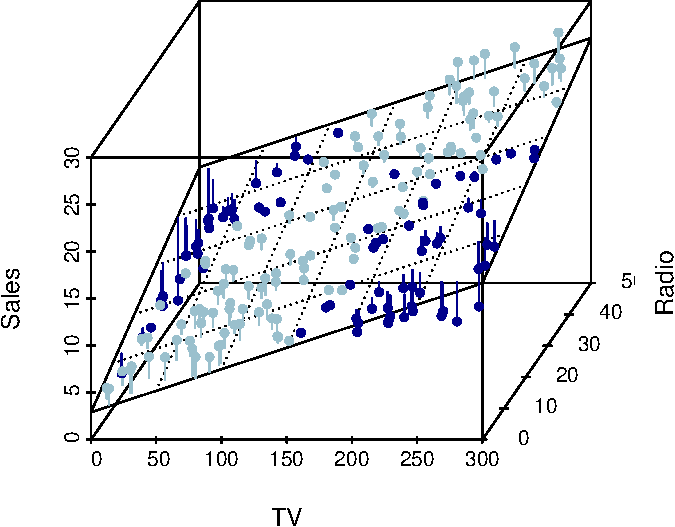
\includegraphics{SDM-CHAP24_files/figure-latex/mucho-1} 

}

\caption{3-D residuals and fitted plane}\label{fig:mucho}
\end{figure}

\hypertarget{using-plotly-1}{%
\subsubsection{\texorpdfstring{Using \texttt{plotly}}{Using plotly}}\label{using-plotly-1}}

\begin{Shaded}
\begin{Highlighting}[]
\FunctionTok{library}\NormalTok{(plotly)}
\CommentTok{\# draw the 3D scatterplot}
\NormalTok{p }\OtherTok{\textless{}{-}} \FunctionTok{plot\_ly}\NormalTok{(}\AttributeTok{data =}\NormalTok{ AD, }\AttributeTok{z =} \SpecialCharTok{\textasciitilde{}}\NormalTok{sales, }\AttributeTok{x =} \SpecialCharTok{\textasciitilde{}}\NormalTok{TV, }\AttributeTok{y =} \SpecialCharTok{\textasciitilde{}}\NormalTok{radio, }\AttributeTok{opacity =} \FloatTok{0.5}\NormalTok{) }\SpecialCharTok{\%\textgreater{}\%} 
\NormalTok{  add\_markers}
\NormalTok{p}
\end{Highlighting}
\end{Shaded}

\begin{center}
\includegraphics{SDM-CHAP24_files/figure-latex/unnamed-chunk-2-1} \end{center}

\begin{Shaded}
\begin{Highlighting}[]
\NormalTok{x }\OtherTok{\textless{}{-}} \FunctionTok{seq}\NormalTok{(}\DecValTok{0}\NormalTok{, }\DecValTok{300}\NormalTok{, }\AttributeTok{length =} \DecValTok{70}\NormalTok{)}
\NormalTok{y }\OtherTok{\textless{}{-}} \FunctionTok{seq}\NormalTok{(}\DecValTok{0}\NormalTok{, }\DecValTok{50}\NormalTok{, }\AttributeTok{length =} \DecValTok{70}\NormalTok{)}
\NormalTok{plane }\OtherTok{\textless{}{-}} \FunctionTok{outer}\NormalTok{(x, y, }\ControlFlowTok{function}\NormalTok{(a, b)\{}\FunctionTok{summary}\NormalTok{(mod2)}\SpecialCharTok{$}\NormalTok{coef[}\DecValTok{1}\NormalTok{, }\DecValTok{1}\NormalTok{] }\SpecialCharTok{+} \FunctionTok{summary}\NormalTok{(mod2)}\SpecialCharTok{$}\NormalTok{coef[}\DecValTok{2}\NormalTok{, }\DecValTok{1}\NormalTok{]}\SpecialCharTok{*}\NormalTok{a }\SpecialCharTok{+} \FunctionTok{summary}\NormalTok{(mod2)}\SpecialCharTok{$}\NormalTok{coef[}\DecValTok{3}\NormalTok{, }\DecValTok{1}\NormalTok{]}\SpecialCharTok{*}\NormalTok{b\})}
\CommentTok{\# draw the plane}
\NormalTok{p }\SpecialCharTok{\%\textgreater{}\%} 
  \FunctionTok{add\_surface}\NormalTok{(}\AttributeTok{x =} \SpecialCharTok{\textasciitilde{}}\NormalTok{x, }\AttributeTok{y =} \SpecialCharTok{\textasciitilde{}}\NormalTok{y, }\AttributeTok{z =} \SpecialCharTok{\textasciitilde{}}\NormalTok{plane, }\AttributeTok{showscale =} \ConstantTok{FALSE}\NormalTok{)}
\end{Highlighting}
\end{Shaded}

\begin{center}
\includegraphics{SDM-CHAP24_files/figure-latex/unnamed-chunk-3-1} \end{center}

\hypertarget{is-there-a-relationship-between-the-response-and-predictors}{%
\subsection{Is There a Relationship Between the Response and Predictors?}\label{is-there-a-relationship-between-the-response-and-predictors}}

\begin{Shaded}
\begin{Highlighting}[]
\NormalTok{mod3 }\OtherTok{\textless{}{-}} \FunctionTok{lm}\NormalTok{(sales }\SpecialCharTok{\textasciitilde{}}\NormalTok{ TV }\SpecialCharTok{+}\NormalTok{ radio }\SpecialCharTok{+}\NormalTok{ newspaper, }\AttributeTok{data =}\NormalTok{ AD)}
\FunctionTok{summary}\NormalTok{(mod3)}
\end{Highlighting}
\end{Shaded}

\begin{verbatim}
Call:
lm(formula = sales ~ TV + radio + newspaper, data = AD)

Residuals:
    Min      1Q  Median      3Q     Max 
-8.8277 -0.8908  0.2418  1.1893  2.8292 

Coefficients:
             Estimate Std. Error t value Pr(>|t|)    
(Intercept)  2.938889   0.311908   9.422   <2e-16 ***
TV           0.045765   0.001395  32.809   <2e-16 ***
radio        0.188530   0.008611  21.893   <2e-16 ***
newspaper   -0.001037   0.005871  -0.177     0.86    
---
Signif. codes:  0 '***' 0.001 '**' 0.01 '*' 0.05 '.' 0.1 ' ' 1

Residual standard error: 1.686 on 196 degrees of freedom
Multiple R-squared:  0.8972,    Adjusted R-squared:  0.8956 
F-statistic: 570.3 on 3 and 196 DF,  p-value: < 2.2e-16
\end{verbatim}

\[H_0: \beta_1 = \beta_2 = \beta_3 = 0\]
versus the alternative
\[H_1: \text{at least one } \beta_j \neq 0\]

The test statistic is \(F = \frac{(\text{TSS} - \text{RSS})/p}{\text{RSS}/(n-p-1)}\)

\begin{Shaded}
\begin{Highlighting}[]
\FunctionTok{anova}\NormalTok{(mod3)}
\end{Highlighting}
\end{Shaded}

\begin{verbatim}
Analysis of Variance Table

Response: sales
           Df Sum Sq Mean Sq   F value Pr(>F)    
TV          1 3314.6  3314.6 1166.7308 <2e-16 ***
radio       1 1545.6  1545.6  544.0501 <2e-16 ***
newspaper   1    0.1     0.1    0.0312 0.8599    
Residuals 196  556.8     2.8                     
---
Signif. codes:  0 '***' 0.001 '**' 0.01 '*' 0.05 '.' 0.1 ' ' 1
\end{verbatim}

\begin{Shaded}
\begin{Highlighting}[]
\NormalTok{SSR }\OtherTok{\textless{}{-}} \FunctionTok{sum}\NormalTok{(}\FunctionTok{anova}\NormalTok{(mod3)[}\DecValTok{1}\SpecialCharTok{:}\DecValTok{3}\NormalTok{, }\DecValTok{2}\NormalTok{])}
\NormalTok{MSR }\OtherTok{\textless{}{-}}\NormalTok{ SSR}\SpecialCharTok{/}\DecValTok{3}
\NormalTok{SSE }\OtherTok{\textless{}{-}} \FunctionTok{anova}\NormalTok{(mod3)[}\DecValTok{4}\NormalTok{, }\DecValTok{2}\NormalTok{]}
\NormalTok{MSE }\OtherTok{\textless{}{-}}\NormalTok{ SSE}\SpecialCharTok{/}\NormalTok{(}\DecValTok{200{-}3{-}1}\NormalTok{)}
\NormalTok{Fobs }\OtherTok{\textless{}{-}}\NormalTok{ MSR}\SpecialCharTok{/}\NormalTok{MSE}
\NormalTok{Fobs}
\end{Highlighting}
\end{Shaded}

\begin{verbatim}
[1] 570.2707
\end{verbatim}

\begin{Shaded}
\begin{Highlighting}[]
\NormalTok{pvalue }\OtherTok{\textless{}{-}} \FunctionTok{pf}\NormalTok{(Fobs, }\DecValTok{3}\NormalTok{, }\DecValTok{196}\NormalTok{, }\AttributeTok{lower =} \ConstantTok{FALSE}\NormalTok{)}
\NormalTok{pvalue}
\end{Highlighting}
\end{Shaded}

\begin{verbatim}
[1] 1.575227e-96
\end{verbatim}

\begin{Shaded}
\begin{Highlighting}[]
\CommentTok{\# Or}
\FunctionTok{summary}\NormalTok{(mod3)}
\end{Highlighting}
\end{Shaded}

\begin{verbatim}
Call:
lm(formula = sales ~ TV + radio + newspaper, data = AD)

Residuals:
    Min      1Q  Median      3Q     Max 
-8.8277 -0.8908  0.2418  1.1893  2.8292 

Coefficients:
             Estimate Std. Error t value Pr(>|t|)    
(Intercept)  2.938889   0.311908   9.422   <2e-16 ***
TV           0.045765   0.001395  32.809   <2e-16 ***
radio        0.188530   0.008611  21.893   <2e-16 ***
newspaper   -0.001037   0.005871  -0.177     0.86    
---
Signif. codes:  0 '***' 0.001 '**' 0.01 '*' 0.05 '.' 0.1 ' ' 1

Residual standard error: 1.686 on 196 degrees of freedom
Multiple R-squared:  0.8972,    Adjusted R-squared:  0.8956 
F-statistic: 570.3 on 3 and 196 DF,  p-value: < 2.2e-16
\end{verbatim}

\begin{Shaded}
\begin{Highlighting}[]
\FunctionTok{summary}\NormalTok{(mod3)}\SpecialCharTok{$}\NormalTok{fstatistic}
\end{Highlighting}
\end{Shaded}

\begin{verbatim}
   value    numdf    dendf 
570.2707   3.0000 196.0000 
\end{verbatim}

Suppose we would like to test whether \(\beta_2 = \beta_3 = 0\). The reduced model with \(\beta_2 = \beta_3 = 0\) is \texttt{mod1} while the full model is \texttt{mod3}.

\begin{Shaded}
\begin{Highlighting}[]
\FunctionTok{summary}\NormalTok{(mod3)}
\end{Highlighting}
\end{Shaded}

\begin{verbatim}
Call:
lm(formula = sales ~ TV + radio + newspaper, data = AD)

Residuals:
    Min      1Q  Median      3Q     Max 
-8.8277 -0.8908  0.2418  1.1893  2.8292 

Coefficients:
             Estimate Std. Error t value Pr(>|t|)    
(Intercept)  2.938889   0.311908   9.422   <2e-16 ***
TV           0.045765   0.001395  32.809   <2e-16 ***
radio        0.188530   0.008611  21.893   <2e-16 ***
newspaper   -0.001037   0.005871  -0.177     0.86    
---
Signif. codes:  0 '***' 0.001 '**' 0.01 '*' 0.05 '.' 0.1 ' ' 1

Residual standard error: 1.686 on 196 degrees of freedom
Multiple R-squared:  0.8972,    Adjusted R-squared:  0.8956 
F-statistic: 570.3 on 3 and 196 DF,  p-value: < 2.2e-16
\end{verbatim}

\begin{Shaded}
\begin{Highlighting}[]
\FunctionTok{anova}\NormalTok{(mod1, mod3)}
\end{Highlighting}
\end{Shaded}

\begin{verbatim}
Analysis of Variance Table

Model 1: sales ~ TV
Model 2: sales ~ TV + radio + newspaper
  Res.Df     RSS Df Sum of Sq      F    Pr(>F)    
1    198 2102.53                                  
2    196  556.83  2    1545.7 272.04 < 2.2e-16 ***
---
Signif. codes:  0 '***' 0.001 '**' 0.01 '*' 0.05 '.' 0.1 ' ' 1
\end{verbatim}

\hypertarget{variable-selection}{%
\subsection{Variable Selection}\label{variable-selection}}

\begin{itemize}
\tightlist
\item
  Forward selection
\end{itemize}

\begin{Shaded}
\begin{Highlighting}[]
\NormalTok{mod.fs }\OtherTok{\textless{}{-}} \FunctionTok{lm}\NormalTok{(sales }\SpecialCharTok{\textasciitilde{}} \DecValTok{1}\NormalTok{, }\AttributeTok{data =}\NormalTok{ AD)}
\NormalTok{SCOPE }\OtherTok{\textless{}{-}}\NormalTok{ (}\SpecialCharTok{\textasciitilde{}}\NormalTok{ TV }\SpecialCharTok{+}\NormalTok{ radio }\SpecialCharTok{+}\NormalTok{ newspaper)}
\FunctionTok{add1}\NormalTok{(mod.fs, }\AttributeTok{scope =}\NormalTok{ SCOPE, }\AttributeTok{test =} \StringTok{"F"}\NormalTok{)}
\end{Highlighting}
\end{Shaded}

\begin{verbatim}
Single term additions

Model:
sales ~ 1
          Df Sum of Sq    RSS    AIC F value    Pr(>F)    
<none>                 5417.1 661.80                      
TV         1    3314.6 2102.5 474.52 312.145 < 2.2e-16 ***
radio      1    1798.7 3618.5 583.10  98.422 < 2.2e-16 ***
newspaper  1     282.3 5134.8 653.10  10.887  0.001148 ** 
---
Signif. codes:  0 '***' 0.001 '**' 0.01 '*' 0.05 '.' 0.1 ' ' 1
\end{verbatim}

\begin{Shaded}
\begin{Highlighting}[]
\NormalTok{mod.fs }\OtherTok{\textless{}{-}} \FunctionTok{update}\NormalTok{(mod.fs, .}\SpecialCharTok{\textasciitilde{}}\NormalTok{. }\SpecialCharTok{+}\NormalTok{ TV)}
\FunctionTok{add1}\NormalTok{(mod.fs, }\AttributeTok{scope =}\NormalTok{ SCOPE, }\AttributeTok{test =} \StringTok{"F"}\NormalTok{)}
\end{Highlighting}
\end{Shaded}

\begin{verbatim}
Single term additions

Model:
sales ~ TV
          Df Sum of Sq     RSS    AIC F value    Pr(>F)    
<none>                 2102.53 474.52                      
radio      1   1545.62  556.91 210.82  546.74 < 2.2e-16 ***
newspaper  1    183.97 1918.56 458.20   18.89 2.217e-05 ***
---
Signif. codes:  0 '***' 0.001 '**' 0.01 '*' 0.05 '.' 0.1 ' ' 1
\end{verbatim}

\begin{Shaded}
\begin{Highlighting}[]
\NormalTok{mod.fs }\OtherTok{\textless{}{-}} \FunctionTok{update}\NormalTok{(mod.fs, .}\SpecialCharTok{\textasciitilde{}}\NormalTok{. }\SpecialCharTok{+}\NormalTok{ radio)}
\FunctionTok{add1}\NormalTok{(mod.fs, }\AttributeTok{scope =}\NormalTok{ SCOPE, }\AttributeTok{test =} \StringTok{"F"}\NormalTok{)}
\end{Highlighting}
\end{Shaded}

\begin{verbatim}
Single term additions

Model:
sales ~ TV + radio
          Df Sum of Sq    RSS    AIC F value Pr(>F)
<none>                 556.91 210.82               
newspaper  1  0.088717 556.83 212.79  0.0312 0.8599
\end{verbatim}

\begin{Shaded}
\begin{Highlighting}[]
\FunctionTok{summary}\NormalTok{(mod.fs)}
\end{Highlighting}
\end{Shaded}

\begin{verbatim}
Call:
lm(formula = sales ~ TV + radio, data = AD)

Residuals:
    Min      1Q  Median      3Q     Max 
-8.7977 -0.8752  0.2422  1.1708  2.8328 

Coefficients:
            Estimate Std. Error t value Pr(>|t|)    
(Intercept)  2.92110    0.29449   9.919   <2e-16 ***
TV           0.04575    0.00139  32.909   <2e-16 ***
radio        0.18799    0.00804  23.382   <2e-16 ***
---
Signif. codes:  0 '***' 0.001 '**' 0.01 '*' 0.05 '.' 0.1 ' ' 1

Residual standard error: 1.681 on 197 degrees of freedom
Multiple R-squared:  0.8972,    Adjusted R-squared:  0.8962 
F-statistic: 859.6 on 2 and 197 DF,  p-value: < 2.2e-16
\end{verbatim}

\begin{itemize}
\tightlist
\item
  Using \texttt{stepAIC}
\end{itemize}

\begin{Shaded}
\begin{Highlighting}[]
\FunctionTok{stepAIC}\NormalTok{(}\FunctionTok{lm}\NormalTok{(sales }\SpecialCharTok{\textasciitilde{}} \DecValTok{1}\NormalTok{, }\AttributeTok{data =}\NormalTok{ AD), }\AttributeTok{scope =}\NormalTok{ (}\SpecialCharTok{\textasciitilde{}}\NormalTok{TV }\SpecialCharTok{+}\NormalTok{ radio }\SpecialCharTok{+}\NormalTok{ newspaper), }\AttributeTok{direction =} \StringTok{"forward"}\NormalTok{, }\AttributeTok{test =} \StringTok{"F"}\NormalTok{)}
\end{Highlighting}
\end{Shaded}

\begin{verbatim}
Start:  AIC=661.8
sales ~ 1

            Df Sum of Sq    RSS    AIC F Value     Pr(F)    
+ TV         1    3314.6 2102.5 474.52 312.145 < 2.2e-16 ***
+ radio      1    1798.7 3618.5 583.10  98.422 < 2.2e-16 ***
+ newspaper  1     282.3 5134.8 653.10  10.887  0.001148 ** 
<none>                   5417.1 661.80                      
---
Signif. codes:  0 '***' 0.001 '**' 0.01 '*' 0.05 '.' 0.1 ' ' 1

Step:  AIC=474.52
sales ~ TV

            Df Sum of Sq     RSS    AIC F Value     Pr(F)    
+ radio      1   1545.62  556.91 210.82  546.74 < 2.2e-16 ***
+ newspaper  1    183.97 1918.56 458.20   18.89 2.217e-05 ***
<none>                   2102.53 474.52                      
---
Signif. codes:  0 '***' 0.001 '**' 0.01 '*' 0.05 '.' 0.1 ' ' 1

Step:  AIC=210.82
sales ~ TV + radio

            Df Sum of Sq    RSS    AIC  F Value  Pr(F)
<none>                   556.91 210.82                
+ newspaper  1  0.088717 556.83 212.79 0.031228 0.8599
\end{verbatim}

\begin{verbatim}
Call:
lm(formula = sales ~ TV + radio, data = AD)

Coefficients:
(Intercept)           TV        radio  
    2.92110      0.04575      0.18799  
\end{verbatim}

\begin{Shaded}
\begin{Highlighting}[]
\CommentTok{\# Or}
\NormalTok{null }\OtherTok{\textless{}{-}} \FunctionTok{lm}\NormalTok{(sales }\SpecialCharTok{\textasciitilde{}} \DecValTok{1}\NormalTok{, }\AttributeTok{data =}\NormalTok{ AD)}
\NormalTok{full }\OtherTok{\textless{}{-}} \FunctionTok{lm}\NormalTok{(sales }\SpecialCharTok{\textasciitilde{}}\NormalTok{ ., }\AttributeTok{data =}\NormalTok{ AD)}
\FunctionTok{stepAIC}\NormalTok{(null, }\AttributeTok{scope =} \FunctionTok{list}\NormalTok{(}\AttributeTok{lower =}\NormalTok{ null, }\AttributeTok{upper =}\NormalTok{ full), }\AttributeTok{direction =} \StringTok{"forward"}\NormalTok{, }\AttributeTok{test =} \StringTok{"F"}\NormalTok{)}
\end{Highlighting}
\end{Shaded}

\begin{verbatim}
Start:  AIC=661.8
sales ~ 1

            Df Sum of Sq    RSS    AIC F Value     Pr(F)    
+ TV         1    3314.6 2102.5 474.52 312.145 < 2.2e-16 ***
+ radio      1    1798.7 3618.5 583.10  98.422 < 2.2e-16 ***
+ newspaper  1     282.3 5134.8 653.10  10.887  0.001148 ** 
<none>                   5417.1 661.80                      
+ X          1      14.4 5402.7 663.27   0.529  0.467917    
---
Signif. codes:  0 '***' 0.001 '**' 0.01 '*' 0.05 '.' 0.1 ' ' 1

Step:  AIC=474.52
sales ~ TV

            Df Sum of Sq     RSS    AIC F Value     Pr(F)    
+ radio      1   1545.62  556.91 210.82  546.74 < 2.2e-16 ***
+ newspaper  1    183.97 1918.56 458.20   18.89 2.217e-05 ***
+ X          1     23.23 2079.30 474.29    2.20    0.1395    
<none>                   2102.53 474.52                      
---
Signif. codes:  0 '***' 0.001 '**' 0.01 '*' 0.05 '.' 0.1 ' ' 1

Step:  AIC=210.82
sales ~ TV + radio

            Df Sum of Sq    RSS    AIC  F Value  Pr(F)
<none>                   556.91 210.82                
+ X          1  0.181080 556.73 212.75 0.063750 0.8009
+ newspaper  1  0.088717 556.83 212.79 0.031228 0.8599
\end{verbatim}

\begin{verbatim}
Call:
lm(formula = sales ~ TV + radio, data = AD)

Coefficients:
(Intercept)           TV        radio  
    2.92110      0.04575      0.18799  
\end{verbatim}

\begin{itemize}
\tightlist
\item
  Backward elimination
\end{itemize}

\begin{Shaded}
\begin{Highlighting}[]
\NormalTok{mod.be }\OtherTok{\textless{}{-}} \FunctionTok{lm}\NormalTok{(sales }\SpecialCharTok{\textasciitilde{}}\NormalTok{ TV }\SpecialCharTok{+}\NormalTok{ radio }\SpecialCharTok{+}\NormalTok{ newspaper, }\AttributeTok{data =}\NormalTok{ AD)}
\FunctionTok{drop1}\NormalTok{(mod.be, }\AttributeTok{test =} \StringTok{"F"}\NormalTok{)}
\end{Highlighting}
\end{Shaded}

\begin{verbatim}
Single term deletions

Model:
sales ~ TV + radio + newspaper
          Df Sum of Sq    RSS    AIC   F value Pr(>F)    
<none>                  556.8 212.79                     
TV         1   3058.01 3614.8 584.90 1076.4058 <2e-16 ***
radio      1   1361.74 1918.6 458.20  479.3252 <2e-16 ***
newspaper  1      0.09  556.9 210.82    0.0312 0.8599    
---
Signif. codes:  0 '***' 0.001 '**' 0.01 '*' 0.05 '.' 0.1 ' ' 1
\end{verbatim}

\begin{Shaded}
\begin{Highlighting}[]
\NormalTok{mod.be }\OtherTok{\textless{}{-}} \FunctionTok{update}\NormalTok{(mod.be, .}\SpecialCharTok{\textasciitilde{}}\NormalTok{. }\SpecialCharTok{{-}}\NormalTok{ newspaper)}
\FunctionTok{drop1}\NormalTok{(mod.be, }\AttributeTok{test =} \StringTok{"F"}\NormalTok{)}
\end{Highlighting}
\end{Shaded}

\begin{verbatim}
Single term deletions

Model:
sales ~ TV + radio
       Df Sum of Sq    RSS    AIC F value    Pr(>F)    
<none>               556.9 210.82                      
TV      1    3061.6 3618.5 583.10 1082.98 < 2.2e-16 ***
radio   1    1545.6 2102.5 474.52  546.74 < 2.2e-16 ***
---
Signif. codes:  0 '***' 0.001 '**' 0.01 '*' 0.05 '.' 0.1 ' ' 1
\end{verbatim}

\begin{Shaded}
\begin{Highlighting}[]
\FunctionTok{summary}\NormalTok{(mod.be)}
\end{Highlighting}
\end{Shaded}

\begin{verbatim}
Call:
lm(formula = sales ~ TV + radio, data = AD)

Residuals:
    Min      1Q  Median      3Q     Max 
-8.7977 -0.8752  0.2422  1.1708  2.8328 

Coefficients:
            Estimate Std. Error t value Pr(>|t|)    
(Intercept)  2.92110    0.29449   9.919   <2e-16 ***
TV           0.04575    0.00139  32.909   <2e-16 ***
radio        0.18799    0.00804  23.382   <2e-16 ***
---
Signif. codes:  0 '***' 0.001 '**' 0.01 '*' 0.05 '.' 0.1 ' ' 1

Residual standard error: 1.681 on 197 degrees of freedom
Multiple R-squared:  0.8972,    Adjusted R-squared:  0.8962 
F-statistic: 859.6 on 2 and 197 DF,  p-value: < 2.2e-16
\end{verbatim}

\begin{itemize}
\tightlist
\item
  Using \texttt{stepAIC}
\end{itemize}

\begin{Shaded}
\begin{Highlighting}[]
\FunctionTok{stepAIC}\NormalTok{(}\FunctionTok{lm}\NormalTok{(sales }\SpecialCharTok{\textasciitilde{}}\NormalTok{ TV }\SpecialCharTok{+}\NormalTok{ radio }\SpecialCharTok{+}\NormalTok{ newspaper, }\AttributeTok{data =}\NormalTok{ AD), }\AttributeTok{scope =}\NormalTok{ (}\SpecialCharTok{\textasciitilde{}}\NormalTok{TV }\SpecialCharTok{+}\NormalTok{ radio }\SpecialCharTok{+}\NormalTok{ newspaper), }\AttributeTok{direction =} \StringTok{"backward"}\NormalTok{, }\AttributeTok{test =} \StringTok{"F"}\NormalTok{)}
\end{Highlighting}
\end{Shaded}

\begin{verbatim}
Start:  AIC=212.79
sales ~ TV + radio + newspaper

            Df Sum of Sq    RSS    AIC F Value  Pr(F)    
- newspaper  1      0.09  556.9 210.82    0.03 0.8599    
<none>                    556.8 212.79                   
- radio      1   1361.74 1918.6 458.20  479.33 <2e-16 ***
- TV         1   3058.01 3614.8 584.90 1076.41 <2e-16 ***
---
Signif. codes:  0 '***' 0.001 '**' 0.01 '*' 0.05 '.' 0.1 ' ' 1

Step:  AIC=210.82
sales ~ TV + radio

        Df Sum of Sq    RSS    AIC F Value     Pr(F)    
<none>                556.9 210.82                      
- radio  1    1545.6 2102.5 474.52  546.74 < 2.2e-16 ***
- TV     1    3061.6 3618.5 583.10 1082.98 < 2.2e-16 ***
---
Signif. codes:  0 '***' 0.001 '**' 0.01 '*' 0.05 '.' 0.1 ' ' 1
\end{verbatim}

\begin{verbatim}
Call:
lm(formula = sales ~ TV + radio, data = AD)

Coefficients:
(Intercept)           TV        radio  
    2.92110      0.04575      0.18799  
\end{verbatim}

\begin{Shaded}
\begin{Highlighting}[]
\CommentTok{\# Or}
\FunctionTok{stepAIC}\NormalTok{(full, }\AttributeTok{scope =} \FunctionTok{list}\NormalTok{(}\AttributeTok{lower =}\NormalTok{ null, }\AttributeTok{upper =}\NormalTok{ full), }\AttributeTok{direction =} \StringTok{"backward"}\NormalTok{, }\AttributeTok{test =} \StringTok{"F"}\NormalTok{)}
\end{Highlighting}
\end{Shaded}

\begin{verbatim}
Start:  AIC=214.71
sales ~ X + TV + radio + newspaper

            Df Sum of Sq    RSS    AIC F Value  Pr(F)    
- newspaper  1      0.13  556.7 212.75    0.04 0.8342    
- X          1      0.22  556.8 212.79    0.08 0.7827    
<none>                    556.6 214.71                   
- radio      1   1354.48 1911.1 459.42  474.52 <2e-16 ***
- TV         1   3056.91 3613.5 586.82 1070.95 <2e-16 ***
---
Signif. codes:  0 '***' 0.001 '**' 0.01 '*' 0.05 '.' 0.1 ' ' 1

Step:  AIC=212.75
sales ~ X + TV + radio

        Df Sum of Sq    RSS    AIC F Value  Pr(F)    
- X      1      0.18  556.9 210.82    0.06 0.8009    
<none>                556.7 212.75                   
- radio  1   1522.57 2079.3 474.29  536.03 <2e-16 ***
- TV     1   3060.94 3617.7 585.05 1077.61 <2e-16 ***
---
Signif. codes:  0 '***' 0.001 '**' 0.01 '*' 0.05 '.' 0.1 ' ' 1

Step:  AIC=210.82
sales ~ TV + radio

        Df Sum of Sq    RSS    AIC F Value     Pr(F)    
<none>                556.9 210.82                      
- radio  1    1545.6 2102.5 474.52  546.74 < 2.2e-16 ***
- TV     1    3061.6 3618.5 583.10 1082.98 < 2.2e-16 ***
---
Signif. codes:  0 '***' 0.001 '**' 0.01 '*' 0.05 '.' 0.1 ' ' 1
\end{verbatim}

\begin{verbatim}
Call:
lm(formula = sales ~ TV + radio, data = AD)

Coefficients:
(Intercept)           TV        radio  
    2.92110      0.04575      0.18799  
\end{verbatim}

\hypertarget{diagnostic-plots}{%
\subsection{Diagnostic Plots}\label{diagnostic-plots}}

\begin{Shaded}
\begin{Highlighting}[]
\FunctionTok{residualPlots}\NormalTok{(mod2)}
\end{Highlighting}
\end{Shaded}

\begin{center}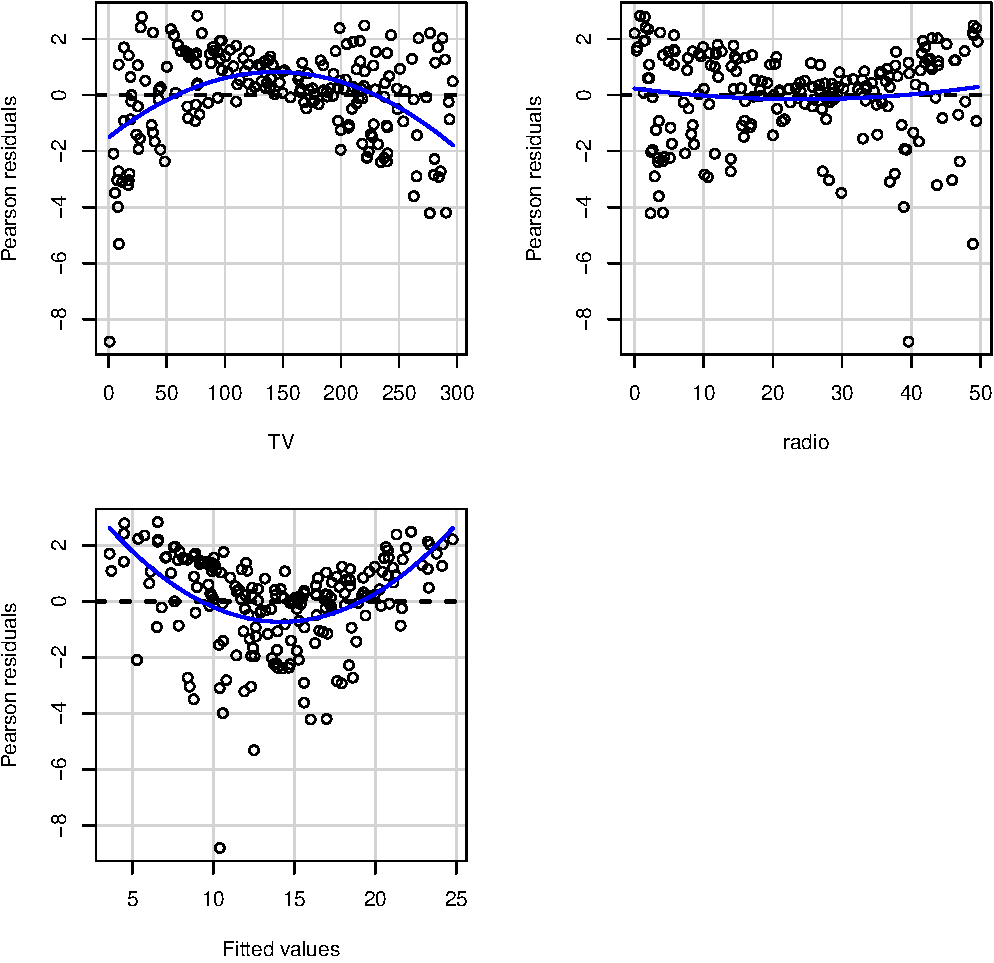
\includegraphics{SDM-CHAP24_files/figure-latex/daignos-1} \end{center}

\begin{verbatim}
           Test stat Pr(>|Test stat|)    
TV           -6.7745        1.423e-10 ***
radio         1.0543           0.2931    
Tukey test    7.6351        2.256e-14 ***
---
Signif. codes:  0 '***' 0.001 '**' 0.01 '*' 0.05 '.' 0.1 ' ' 1
\end{verbatim}

\begin{Shaded}
\begin{Highlighting}[]
\FunctionTok{qqPlot}\NormalTok{(mod2)}
\end{Highlighting}
\end{Shaded}

\begin{center}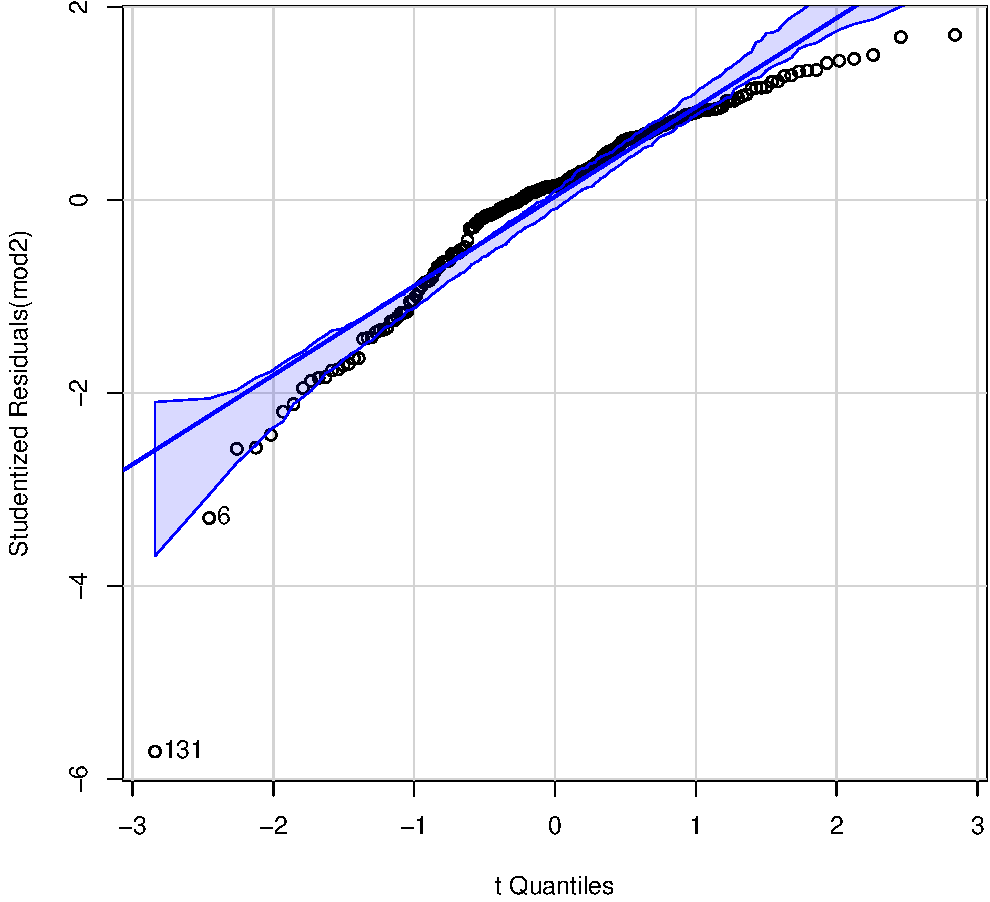
\includegraphics{SDM-CHAP24_files/figure-latex/daignos-2} \end{center}

\begin{verbatim}
[1]   6 131
\end{verbatim}

\begin{Shaded}
\begin{Highlighting}[]
\FunctionTok{influenceIndexPlot}\NormalTok{(mod2)}
\end{Highlighting}
\end{Shaded}

\begin{center}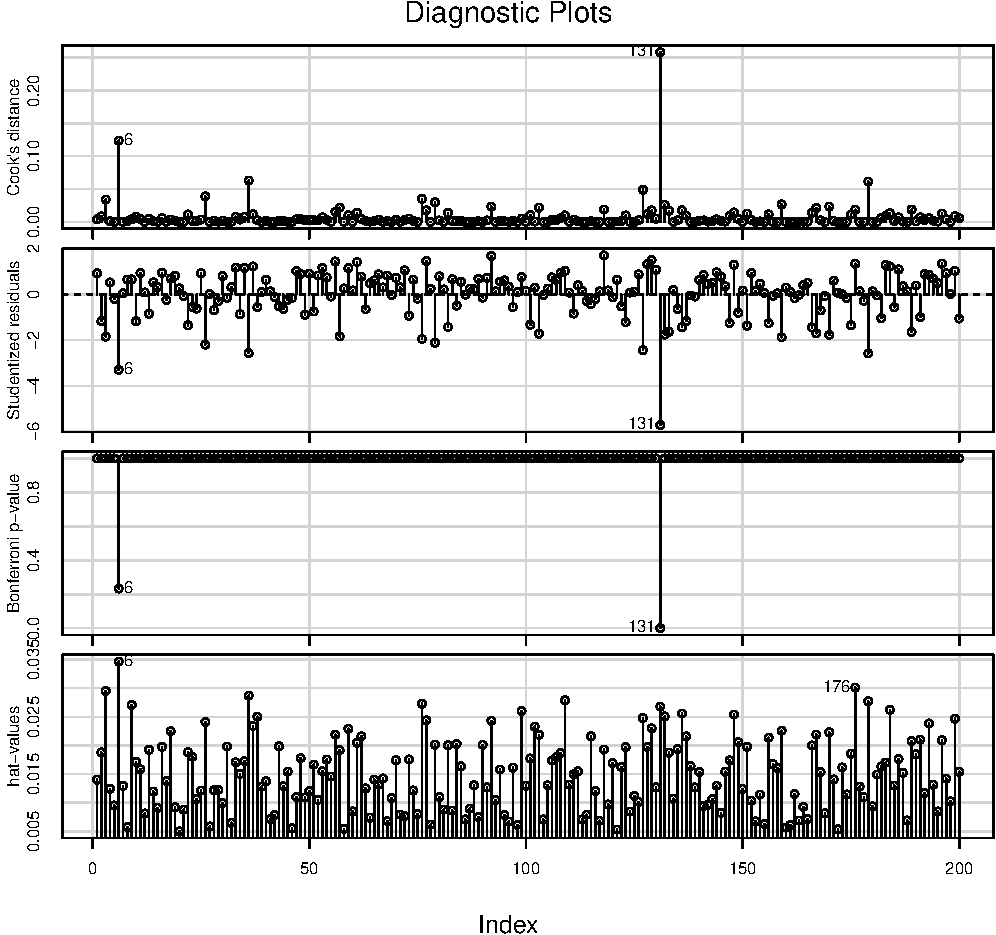
\includegraphics{SDM-CHAP24_files/figure-latex/daignos-3} \end{center}

We use a \emph{confidence interval} to quantify the uncertainty surrounding the \emph{average} \texttt{sales} over a large number of cities. For example, given that \$100,000 is spent on \texttt{TV} advertising and \$20,000 is spent on \texttt{Radio} advertising in each city, the 95\% confidence interval is {[}10.9852544, 11.5276775{]}. We interpret this to mean that 95\% of intervals of this form will contain the true value of \texttt{Sales}.

\begin{Shaded}
\begin{Highlighting}[]
\FunctionTok{predict}\NormalTok{(mod.be, }\AttributeTok{newdata =} \FunctionTok{data.frame}\NormalTok{(}\AttributeTok{TV =} \DecValTok{100}\NormalTok{, }\AttributeTok{radio =} \DecValTok{20}\NormalTok{), }\AttributeTok{interval =} \StringTok{"conf"}\NormalTok{)}
\end{Highlighting}
\end{Shaded}

\begin{verbatim}
       fit      lwr      upr
1 11.25647 10.98525 11.52768
\end{verbatim}

On the other hand, a \emph{prediction interval} can be used to quantify the uncertainty surrounding \texttt{sales} for a \emph{particular} city. Given that \$100,000 is spent on \texttt{TV} advertising and \$20,000 is spent on \texttt{radio} advertising in \textbf{a particular} city, the 95\% prediction interval is {[}7.9296161, 14.5833158{]}. We interpret this to mean that 95\% of intervals of this form will contain the true value of \texttt{Sales} for this city.

\begin{Shaded}
\begin{Highlighting}[]
\FunctionTok{predict}\NormalTok{(mod.be, }\AttributeTok{newdata =} \FunctionTok{data.frame}\NormalTok{(}\AttributeTok{TV =} \DecValTok{100}\NormalTok{, }\AttributeTok{radio =} \DecValTok{20}\NormalTok{), }\AttributeTok{interval =} \StringTok{"pred"}\NormalTok{)}
\end{Highlighting}
\end{Shaded}

\begin{verbatim}
       fit      lwr      upr
1 11.25647 7.929616 14.58332
\end{verbatim}

Note that both the intervals are centered at 11.256466, but that the prediction interval is substantially wider than the confidence interval, reflecting the increased uncertainty about \texttt{Sales} for a given city in comparison to the average \texttt{sales} over many locations.

\hypertarget{non-additive-models}{%
\subsection{Non-Additive Models}\label{non-additive-models}}

\begin{Shaded}
\begin{Highlighting}[]
\NormalTok{nam1 }\OtherTok{\textless{}{-}} \FunctionTok{lm}\NormalTok{(sales }\SpecialCharTok{\textasciitilde{}}\NormalTok{ TV}\SpecialCharTok{*}\NormalTok{radio, }\AttributeTok{data =}\NormalTok{ AD)}
\CommentTok{\# Same as }
\NormalTok{nam2 }\OtherTok{\textless{}{-}} \FunctionTok{lm}\NormalTok{(sales }\SpecialCharTok{\textasciitilde{}}\NormalTok{ TV }\SpecialCharTok{+}\NormalTok{ radio }\SpecialCharTok{+}\NormalTok{ TV}\SpecialCharTok{:}\NormalTok{radio, }\AttributeTok{data =}\NormalTok{ AD)}
\FunctionTok{summary}\NormalTok{(nam1)}
\end{Highlighting}
\end{Shaded}

\begin{verbatim}
Call:
lm(formula = sales ~ TV * radio, data = AD)

Residuals:
    Min      1Q  Median      3Q     Max 
-6.3366 -0.4028  0.1831  0.5948  1.5246 

Coefficients:
             Estimate Std. Error t value Pr(>|t|)    
(Intercept) 6.750e+00  2.479e-01  27.233   <2e-16 ***
TV          1.910e-02  1.504e-03  12.699   <2e-16 ***
radio       2.886e-02  8.905e-03   3.241   0.0014 ** 
TV:radio    1.086e-03  5.242e-05  20.727   <2e-16 ***
---
Signif. codes:  0 '***' 0.001 '**' 0.01 '*' 0.05 '.' 0.1 ' ' 1

Residual standard error: 0.9435 on 196 degrees of freedom
Multiple R-squared:  0.9678,    Adjusted R-squared:  0.9673 
F-statistic:  1963 on 3 and 196 DF,  p-value: < 2.2e-16
\end{verbatim}

\begin{Shaded}
\begin{Highlighting}[]
\FunctionTok{summary}\NormalTok{(nam2)}
\end{Highlighting}
\end{Shaded}

\begin{verbatim}
Call:
lm(formula = sales ~ TV + radio + TV:radio, data = AD)

Residuals:
    Min      1Q  Median      3Q     Max 
-6.3366 -0.4028  0.1831  0.5948  1.5246 

Coefficients:
             Estimate Std. Error t value Pr(>|t|)    
(Intercept) 6.750e+00  2.479e-01  27.233   <2e-16 ***
TV          1.910e-02  1.504e-03  12.699   <2e-16 ***
radio       2.886e-02  8.905e-03   3.241   0.0014 ** 
TV:radio    1.086e-03  5.242e-05  20.727   <2e-16 ***
---
Signif. codes:  0 '***' 0.001 '**' 0.01 '*' 0.05 '.' 0.1 ' ' 1

Residual standard error: 0.9435 on 196 degrees of freedom
Multiple R-squared:  0.9678,    Adjusted R-squared:  0.9673 
F-statistic:  1963 on 3 and 196 DF,  p-value: < 2.2e-16
\end{verbatim}

\textbf{Hierarchical Principle:} If an interaction term is included in a model, one should also include the main effects, even if the \emph{p-values} associated with their coefficients are not significant.

\hypertarget{qualitative-predictors}{%
\subsection{Qualitative Predictors}\label{qualitative-predictors}}

In the \texttt{Credit} data frame there are four qualitative features/variables \texttt{Gender}, \texttt{Student}, \texttt{Married}, and \texttt{Ethnicity}.

\begin{Shaded}
\begin{Highlighting}[]
\NormalTok{Credit }\OtherTok{\textless{}{-}} \FunctionTok{read.csv}\NormalTok{(}\StringTok{"http://statlearning.com/s/Credit.csv"}\NormalTok{)}
\FunctionTok{datatable}\NormalTok{(Credit[, }\SpecialCharTok{{-}}\DecValTok{1}\NormalTok{], }\AttributeTok{rownames =} \ConstantTok{FALSE}\NormalTok{)}
\end{Highlighting}
\end{Shaded}

\begin{center}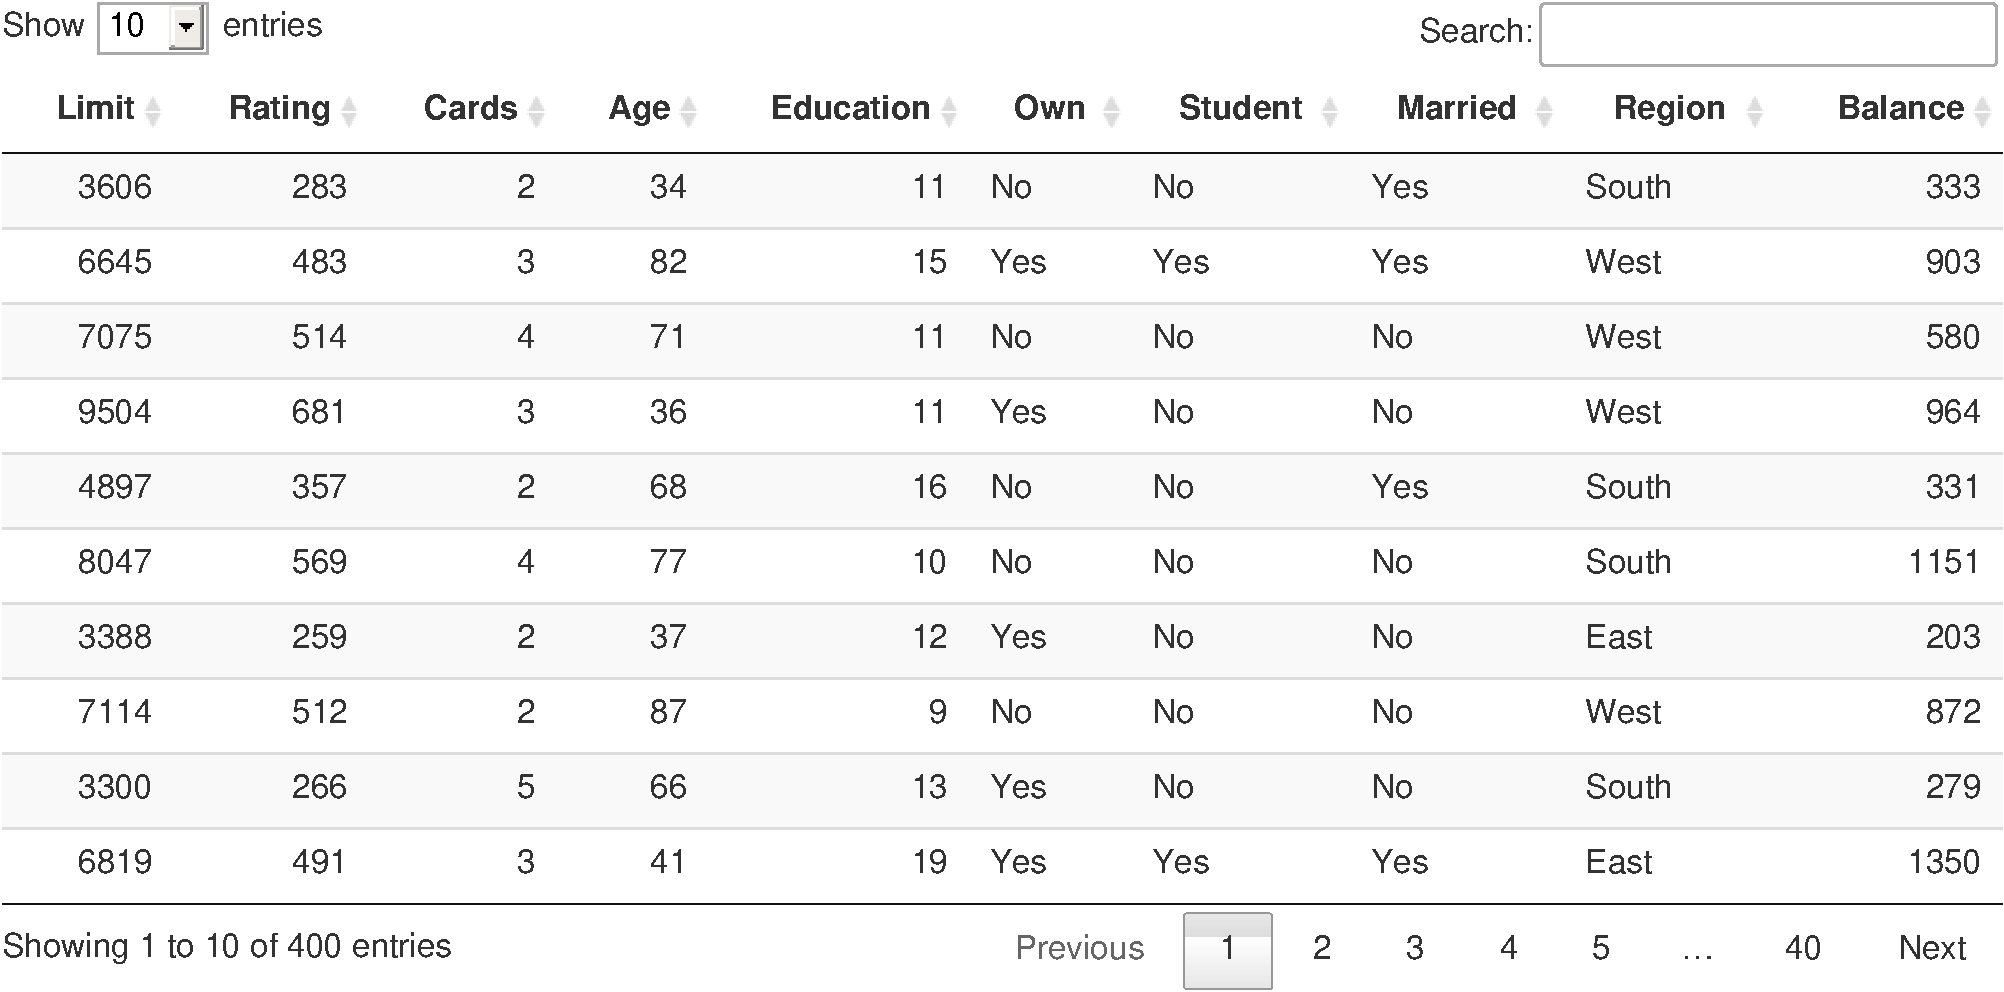
\includegraphics{SDM-CHAP24_files/figure-latex/readin2-1} \end{center}

\begin{Shaded}
\begin{Highlighting}[]
\NormalTok{modP }\OtherTok{\textless{}{-}} \FunctionTok{lm}\NormalTok{(Balance }\SpecialCharTok{\textasciitilde{}}\NormalTok{ Income}\SpecialCharTok{*}\NormalTok{Student, }\AttributeTok{data =}\NormalTok{ Credit)}
\FunctionTok{summary}\NormalTok{(modP)}
\end{Highlighting}
\end{Shaded}

\begin{verbatim}
Call:
lm(formula = Balance ~ Income * Student, data = Credit)

Residuals:
    Min      1Q  Median      3Q     Max 
-773.39 -325.70  -41.13  321.65  814.04 

Coefficients:
                  Estimate Std. Error t value Pr(>|t|)    
(Intercept)       200.6232    33.6984   5.953 5.79e-09 ***
Income              6.2182     0.5921  10.502  < 2e-16 ***
StudentYes        476.6758   104.3512   4.568 6.59e-06 ***
Income:StudentYes  -1.9992     1.7313  -1.155    0.249    
---
Signif. codes:  0 '***' 0.001 '**' 0.01 '*' 0.05 '.' 0.1 ' ' 1

Residual standard error: 391.6 on 396 degrees of freedom
Multiple R-squared:  0.2799,    Adjusted R-squared:  0.2744 
F-statistic:  51.3 on 3 and 396 DF,  p-value: < 2.2e-16
\end{verbatim}

Fitted Model: \(\widehat{\text{Balance}} = 200.6231529 + 6.2181687\cdot \text{Income} + 476.6758432\cdot \text{Student} -1.9991509\cdot\text{Income}\times\text{Student}\)

\hypertarget{predictors-with-only-two-levels}{%
\subsubsection{Predictors with Only Two Levels}\label{predictors-with-only-two-levels}}

Suppose we wish to investigate differences in credit card balance between males and females, ignoring the other variables for the moment.

\begin{Shaded}
\begin{Highlighting}[]
\FunctionTok{library}\NormalTok{(ISLR)}
\FunctionTok{data}\NormalTok{(Credit)}
\NormalTok{modS }\OtherTok{\textless{}{-}} \FunctionTok{lm}\NormalTok{(Balance }\SpecialCharTok{\textasciitilde{}}\NormalTok{ Gender, }\AttributeTok{data =}\NormalTok{ Credit)}
\FunctionTok{summary}\NormalTok{(modS)}
\end{Highlighting}
\end{Shaded}

\begin{verbatim}
Call:
lm(formula = Balance ~ Gender, data = Credit)

Residuals:
    Min      1Q  Median      3Q     Max 
-529.54 -455.35  -60.17  334.71 1489.20 

Coefficients:
             Estimate Std. Error t value Pr(>|t|)    
(Intercept)    509.80      33.13  15.389   <2e-16 ***
GenderFemale    19.73      46.05   0.429    0.669    
---
Signif. codes:  0 '***' 0.001 '**' 0.01 '*' 0.05 '.' 0.1 ' ' 1

Residual standard error: 460.2 on 398 degrees of freedom
Multiple R-squared:  0.0004611, Adjusted R-squared:  -0.00205 
F-statistic: 0.1836 on 1 and 398 DF,  p-value: 0.6685
\end{verbatim}

\begin{Shaded}
\begin{Highlighting}[]
\FunctionTok{coef}\NormalTok{(modS)}
\end{Highlighting}
\end{Shaded}

\begin{verbatim}
 (Intercept) GenderFemale 
   509.80311     19.73312 
\end{verbatim}

\begin{Shaded}
\begin{Highlighting}[]
\FunctionTok{tapply}\NormalTok{(Credit}\SpecialCharTok{$}\NormalTok{Balance, Credit}\SpecialCharTok{$}\NormalTok{Gender, mean)}
\end{Highlighting}
\end{Shaded}

\begin{verbatim}
    Male   Female 
509.8031 529.5362 
\end{verbatim}

\begin{Shaded}
\begin{Highlighting}[]
\FunctionTok{library}\NormalTok{(ggplot2)}
\FunctionTok{ggplot}\NormalTok{(}\AttributeTok{data =}\NormalTok{ Credit, }\FunctionTok{aes}\NormalTok{(}\AttributeTok{x =}\NormalTok{ Gender, }\AttributeTok{y =}\NormalTok{ Balance)) }\SpecialCharTok{+} 
  \FunctionTok{geom\_point}\NormalTok{() }\SpecialCharTok{+} 
  \FunctionTok{theme\_bw}\NormalTok{() }\SpecialCharTok{+} 
  \FunctionTok{geom\_hline}\NormalTok{(}\AttributeTok{yintercept =} \FunctionTok{coef}\NormalTok{(modS)[}\DecValTok{1}\NormalTok{] }\SpecialCharTok{+} \FunctionTok{coef}\NormalTok{(modS)[}\DecValTok{2}\NormalTok{], }\AttributeTok{color =} \StringTok{"purple"}\NormalTok{) }\SpecialCharTok{+} 
  \FunctionTok{geom\_hline}\NormalTok{(}\AttributeTok{yintercept =} \FunctionTok{coef}\NormalTok{(modS)[}\DecValTok{1}\NormalTok{], }\AttributeTok{color =} \StringTok{"green"}\NormalTok{)}
\end{Highlighting}
\end{Shaded}

\begin{center}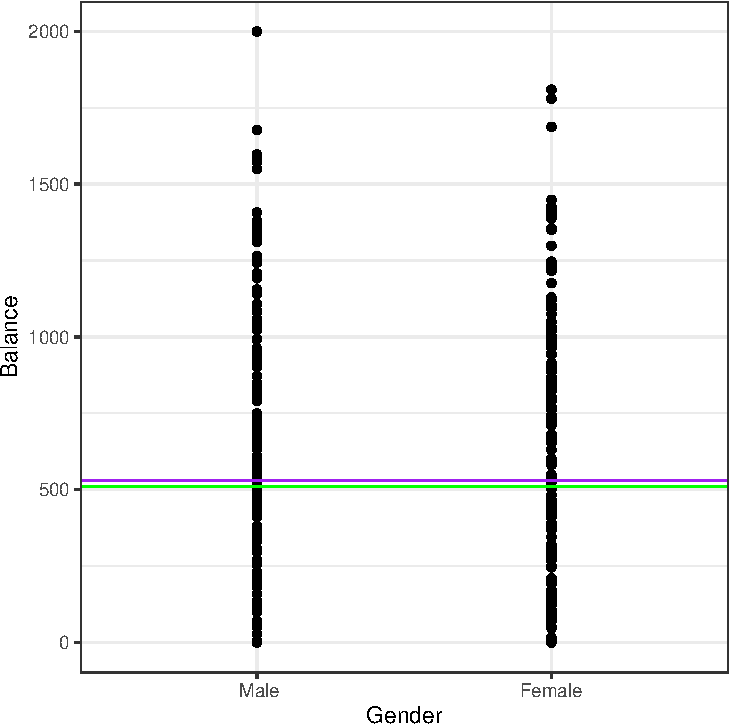
\includegraphics{SDM-CHAP24_files/figure-latex/GGSD-1} \end{center}

Do females have a higher ratio of \texttt{Balance} to \texttt{Income} (credit utilization)? Here is an article from the \href{https://www.washingtonpost.com/news/get-there/wp/2016/02/17/how-being-a-woman-can-ding-your-credit-score/}{Washington Post} with numbers that mirror some of the results in the \texttt{Credit} data set.

\begin{Shaded}
\begin{Highlighting}[]
\NormalTok{Credit}\SpecialCharTok{$}\NormalTok{Utilization }\OtherTok{\textless{}{-}}\NormalTok{ Credit}\SpecialCharTok{$}\NormalTok{Balance }\SpecialCharTok{/}\NormalTok{ (Credit}\SpecialCharTok{$}\NormalTok{Income}\SpecialCharTok{*}\DecValTok{100}\NormalTok{)}
\FunctionTok{tapply}\NormalTok{(Credit}\SpecialCharTok{$}\NormalTok{Utilization, Credit}\SpecialCharTok{$}\NormalTok{Gender, mean)}
\end{Highlighting}
\end{Shaded}

\begin{verbatim}
     Male    Female 
0.1487092 0.1535206 
\end{verbatim}

\begin{Shaded}
\begin{Highlighting}[]
\CommentTok{\# Tidyverse approach}
\NormalTok{Credit }\SpecialCharTok{\%\textgreater{}\%}
  \FunctionTok{mutate}\NormalTok{(}\AttributeTok{Ratio =}\NormalTok{ Balance }\SpecialCharTok{/}\NormalTok{ (Income}\SpecialCharTok{*}\DecValTok{100}\NormalTok{) ) }\SpecialCharTok{\%\textgreater{}\%}
  \FunctionTok{group\_by}\NormalTok{(Gender) }\SpecialCharTok{\%\textgreater{}\%}
  \FunctionTok{summarize}\NormalTok{(}\FunctionTok{mean}\NormalTok{(Ratio))}
\end{Highlighting}
\end{Shaded}

\begin{verbatim}
# A tibble: 2 x 2
  Gender   `mean(Ratio)`
  <fct>            <dbl>
1 " Male"          0.149
2 "Female"         0.154
\end{verbatim}

\begin{Shaded}
\begin{Highlighting}[]
\NormalTok{modU }\OtherTok{\textless{}{-}} \FunctionTok{lm}\NormalTok{(Utilization }\SpecialCharTok{\textasciitilde{}}\NormalTok{ Gender, }\AttributeTok{data =}\NormalTok{ Credit)}
\FunctionTok{summary}\NormalTok{(modU)}
\end{Highlighting}
\end{Shaded}

\begin{verbatim}
Call:
lm(formula = Utilization ~ Gender, data = Credit)

Residuals:
     Min       1Q   Median       3Q      Max 
-0.15352 -0.13494 -0.05202  0.06069  0.96804 

Coefficients:
             Estimate Std. Error t value Pr(>|t|)    
(Intercept)  0.148709   0.012388  12.004   <2e-16 ***
GenderFemale 0.004811   0.017221   0.279     0.78    
---
Signif. codes:  0 '***' 0.001 '**' 0.01 '*' 0.05 '.' 0.1 ' ' 1

Residual standard error: 0.1721 on 398 degrees of freedom
Multiple R-squared:  0.0001961, Adjusted R-squared:  -0.002316 
F-statistic: 0.07806 on 1 and 398 DF,  p-value: 0.7801
\end{verbatim}

\begin{Shaded}
\begin{Highlighting}[]
\FunctionTok{coef}\NormalTok{(modU)}
\end{Highlighting}
\end{Shaded}

\begin{verbatim}
 (Intercept) GenderFemale 
 0.148709165  0.004811408 
\end{verbatim}

\begin{Shaded}
\begin{Highlighting}[]
\FunctionTok{ggplot}\NormalTok{(}\AttributeTok{data =}\NormalTok{ Credit, }\FunctionTok{aes}\NormalTok{(}\AttributeTok{x =}\NormalTok{ Gender, }\AttributeTok{y =}\NormalTok{ Utilization)) }\SpecialCharTok{+} 
  \FunctionTok{geom\_point}\NormalTok{() }\SpecialCharTok{+} 
  \FunctionTok{theme\_bw}\NormalTok{() }\SpecialCharTok{+} 
  \FunctionTok{geom\_hline}\NormalTok{(}\AttributeTok{yintercept =} \FunctionTok{coef}\NormalTok{(modU)[}\DecValTok{1}\NormalTok{] }\SpecialCharTok{+} \FunctionTok{coef}\NormalTok{(modU)[}\DecValTok{2}\NormalTok{], }\AttributeTok{color =} \StringTok{"purple"}\NormalTok{) }\SpecialCharTok{+} 
  \FunctionTok{geom\_hline}\NormalTok{(}\AttributeTok{yintercept =} \FunctionTok{coef}\NormalTok{(modU)[}\DecValTok{1}\NormalTok{], }\AttributeTok{color =} \StringTok{"green"}\NormalTok{)}
\end{Highlighting}
\end{Shaded}

\begin{center}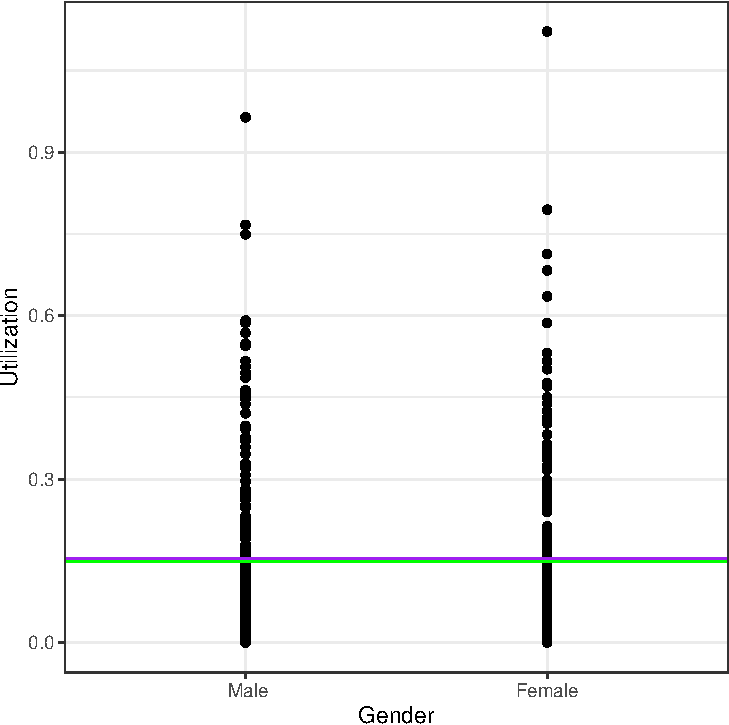
\includegraphics{SDM-CHAP24_files/figure-latex/UTIL-1} \end{center}

\hypertarget{moving-on-now}{%
\subsection{Moving On Now}\label{moving-on-now}}

\begin{Shaded}
\begin{Highlighting}[]
\NormalTok{modS1 }\OtherTok{\textless{}{-}} \FunctionTok{lm}\NormalTok{(Balance }\SpecialCharTok{\textasciitilde{}}\NormalTok{ Limit }\SpecialCharTok{+}\NormalTok{ Student, }\AttributeTok{data =}\NormalTok{ Credit)}
\FunctionTok{summary}\NormalTok{(modS1)}
\end{Highlighting}
\end{Shaded}

\begin{verbatim}
Call:
lm(formula = Balance ~ Limit + Student, data = Credit)

Residuals:
    Min      1Q  Median      3Q     Max 
-637.77 -116.90    6.04  130.92  434.24 

Coefficients:
              Estimate Std. Error t value Pr(>|t|)    
(Intercept) -3.347e+02  2.307e+01  -14.51   <2e-16 ***
Limit        1.720e-01  4.331e-03   39.70   <2e-16 ***
StudentYes   4.044e+02  3.328e+01   12.15   <2e-16 ***
---
Signif. codes:  0 '***' 0.001 '**' 0.01 '*' 0.05 '.' 0.1 ' ' 1

Residual standard error: 199.7 on 397 degrees of freedom
Multiple R-squared:  0.8123,    Adjusted R-squared:  0.8114 
F-statistic: 859.2 on 2 and 397 DF,  p-value: < 2.2e-16
\end{verbatim}

\begin{Shaded}
\begin{Highlighting}[]
\FunctionTok{coef}\NormalTok{(modS1)}
\end{Highlighting}
\end{Shaded}

\begin{verbatim}
 (Intercept)        Limit   StudentYes 
-334.7299372    0.1719538  404.4036438 
\end{verbatim}

\begin{Shaded}
\begin{Highlighting}[]
\CommentTok{\# Interaction {-}{-}{-} Non{-}additive Model}
\NormalTok{modS2 }\OtherTok{\textless{}{-}} \FunctionTok{lm}\NormalTok{(Balance }\SpecialCharTok{\textasciitilde{}}\NormalTok{ Limit}\SpecialCharTok{*}\NormalTok{Student, }\AttributeTok{data =}\NormalTok{ Credit)}
\FunctionTok{summary}\NormalTok{(modS2)}
\end{Highlighting}
\end{Shaded}

\begin{verbatim}
Call:
lm(formula = Balance ~ Limit * Student, data = Credit)

Residuals:
    Min      1Q  Median      3Q     Max 
-705.84 -116.90    6.91  133.97  435.92 

Coefficients:
                   Estimate Std. Error t value Pr(>|t|)    
(Intercept)      -3.262e+02  2.392e+01 -13.636  < 2e-16 ***
Limit             1.702e-01  4.533e-03  37.538  < 2e-16 ***
StudentYes        3.091e+02  7.878e+01   3.924 0.000103 ***
Limit:StudentYes  2.028e-02  1.520e-02   1.334 0.183010    
---
Signif. codes:  0 '***' 0.001 '**' 0.01 '*' 0.05 '.' 0.1 ' ' 1

Residual standard error: 199.5 on 396 degrees of freedom
Multiple R-squared:  0.8132,    Adjusted R-squared:  0.8118 
F-statistic: 574.5 on 3 and 396 DF,  p-value: < 2.2e-16
\end{verbatim}

\hypertarget{what-does-this-look-like}{%
\subsubsection{What does this look like?}\label{what-does-this-look-like}}

Several points:

\begin{itemize}
\tightlist
\item
  Is the interaction significant?
\item
  Which model is \texttt{ggplot2} graphing below?
\item
  Is this the correct model?
\end{itemize}

\begin{Shaded}
\begin{Highlighting}[]
\FunctionTok{ggplot}\NormalTok{(}\AttributeTok{data =}\NormalTok{ Credit, }\FunctionTok{aes}\NormalTok{(}\AttributeTok{x =}\NormalTok{ Limit, }\AttributeTok{y =}\NormalTok{ Balance, }\AttributeTok{color =}\NormalTok{ Student)) }\SpecialCharTok{+} 
  \FunctionTok{geom\_point}\NormalTok{() }\SpecialCharTok{+} 
  \FunctionTok{stat\_smooth}\NormalTok{(}\AttributeTok{method =} \StringTok{"lm"}\NormalTok{) }\SpecialCharTok{+} 
  \FunctionTok{theme\_bw}\NormalTok{()}
\end{Highlighting}
\end{Shaded}

\begin{figure}

{\centering 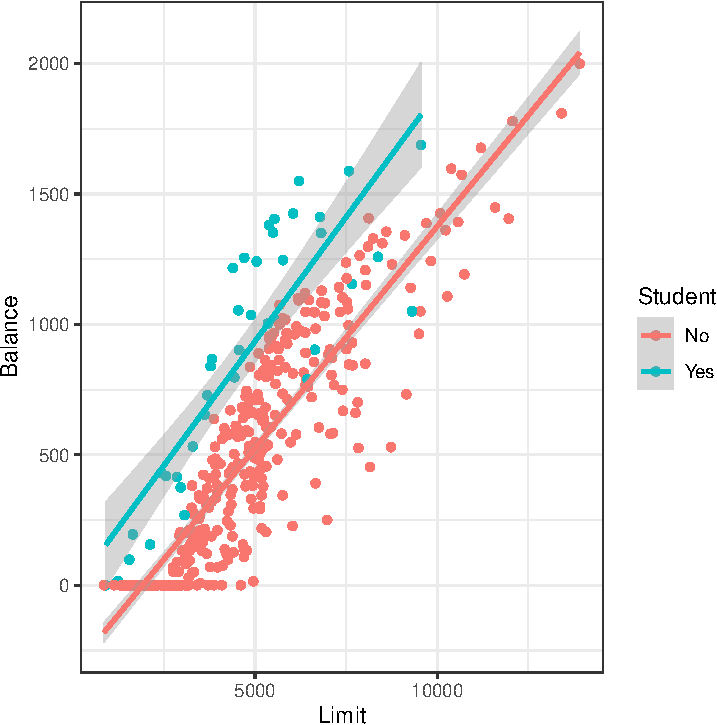
\includegraphics{SDM-CHAP24_files/figure-latex/GGDWDYE-1} 

}

\caption{Balance versus Limit}\label{fig:GGDWDYE}
\end{figure}

\hypertarget{correct-graph}{%
\subsubsection{Correct Graph}\label{correct-graph}}

\begin{Shaded}
\begin{Highlighting}[]
\NormalTok{S2M }\OtherTok{\textless{}{-}} \FunctionTok{lm}\NormalTok{(Balance }\SpecialCharTok{\textasciitilde{}}\NormalTok{ Limit }\SpecialCharTok{+}\NormalTok{ Student, }\AttributeTok{data =}\NormalTok{ Credit)}
\CommentTok{\#}
\FunctionTok{ggplot}\NormalTok{(}\AttributeTok{data =}\NormalTok{ Credit, }\FunctionTok{aes}\NormalTok{(}\AttributeTok{x =}\NormalTok{ Limit, }\AttributeTok{y =}\NormalTok{ Balance, }\AttributeTok{color =}\NormalTok{ Student)) }\SpecialCharTok{+}
  \FunctionTok{geom\_point}\NormalTok{() }\SpecialCharTok{+} 
  \FunctionTok{theme\_bw}\NormalTok{() }\SpecialCharTok{+} 
  \FunctionTok{geom\_abline}\NormalTok{(}\AttributeTok{intercept =} \FunctionTok{coef}\NormalTok{(S2M)[}\DecValTok{1}\NormalTok{], }\AttributeTok{slope =} \FunctionTok{coef}\NormalTok{(S2M)[}\DecValTok{2}\NormalTok{], }\AttributeTok{color =} \StringTok{"red"}\NormalTok{) }\SpecialCharTok{+} 
  \FunctionTok{geom\_abline}\NormalTok{(}\AttributeTok{intercept =} \FunctionTok{coef}\NormalTok{(S2M)[}\DecValTok{1}\NormalTok{] }\SpecialCharTok{+} \FunctionTok{coef}\NormalTok{(S2M)[}\DecValTok{3}\NormalTok{], }\AttributeTok{slope =} \FunctionTok{coef}\NormalTok{(S2M)[}\DecValTok{2}\NormalTok{], }\AttributeTok{color =} \StringTok{"blue"}\NormalTok{) }\SpecialCharTok{+} 
  \FunctionTok{scale\_color\_manual}\NormalTok{(}\AttributeTok{values =} \FunctionTok{c}\NormalTok{(}\StringTok{"red"}\NormalTok{, }\StringTok{"blue"}\NormalTok{))}
\end{Highlighting}
\end{Shaded}

\begin{figure}

{\centering 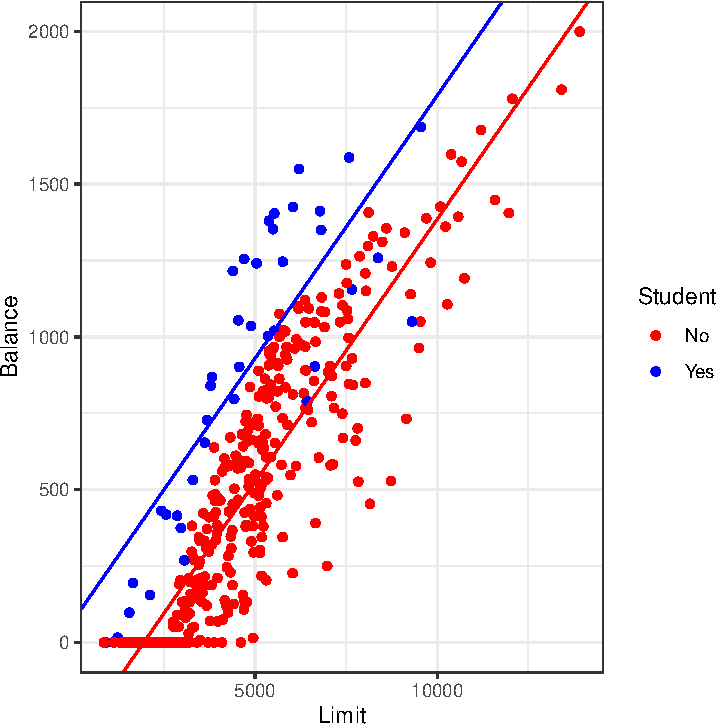
\includegraphics{SDM-CHAP24_files/figure-latex/CG-1} 

}

\caption{Figure this one out!}\label{fig:CG}
\end{figure}

\hypertarget{qualitative-predictors-with-more-than-two-levels}{%
\subsubsection{Qualitative predictors with More than Two Levels}\label{qualitative-predictors-with-more-than-two-levels}}

\begin{Shaded}
\begin{Highlighting}[]
\NormalTok{modQ3 }\OtherTok{\textless{}{-}} \FunctionTok{lm}\NormalTok{(Balance }\SpecialCharTok{\textasciitilde{}}\NormalTok{ Limit }\SpecialCharTok{+}\NormalTok{ Ethnicity, }\AttributeTok{data =}\NormalTok{ Credit)}
\FunctionTok{summary}\NormalTok{(modQ3)}
\end{Highlighting}
\end{Shaded}

\begin{verbatim}
Call:
lm(formula = Balance ~ Limit + Ethnicity, data = Credit)

Residuals:
    Min      1Q  Median      3Q     Max 
-677.39 -145.75   -8.75  139.56  776.46 

Coefficients:
                     Estimate Std. Error t value Pr(>|t|)    
(Intercept)        -3.078e+02  3.417e+01  -9.007   <2e-16 ***
Limit               1.718e-01  5.079e-03  33.831   <2e-16 ***
EthnicityAsian      2.835e+01  3.304e+01   0.858    0.391    
EthnicityCaucasian  1.381e+01  2.878e+01   0.480    0.632    
---
Signif. codes:  0 '***' 0.001 '**' 0.01 '*' 0.05 '.' 0.1 ' ' 1

Residual standard error: 234 on 396 degrees of freedom
Multiple R-squared:  0.743, Adjusted R-squared:  0.7411 
F-statistic: 381.6 on 3 and 396 DF,  p-value: < 2.2e-16
\end{verbatim}

\begin{Shaded}
\begin{Highlighting}[]
\FunctionTok{coef}\NormalTok{(modQ3)}
\end{Highlighting}
\end{Shaded}

\begin{verbatim}
       (Intercept)              Limit     EthnicityAsian EthnicityCaucasian 
      -307.7574777          0.1718203         28.3533975         13.8089629 
\end{verbatim}

\begin{Shaded}
\begin{Highlighting}[]
\NormalTok{modRM }\OtherTok{\textless{}{-}} \FunctionTok{lm}\NormalTok{(Balance }\SpecialCharTok{\textasciitilde{}}\NormalTok{ Limit, }\AttributeTok{data =}\NormalTok{ Credit)}
\FunctionTok{anova}\NormalTok{(modRM, modQ3)}
\end{Highlighting}
\end{Shaded}

\begin{verbatim}
Analysis of Variance Table

Model 1: Balance ~ Limit
Model 2: Balance ~ Limit + Ethnicity
  Res.Df      RSS Df Sum of Sq      F Pr(>F)
1    398 21715657                           
2    396 21675307  2     40350 0.3686 0.6919
\end{verbatim}

What follows fits three separate regression lines based on \texttt{Ethnicity}.

\begin{Shaded}
\begin{Highlighting}[]
\NormalTok{AfAmer }\OtherTok{\textless{}{-}} \FunctionTok{lm}\NormalTok{(Balance }\SpecialCharTok{\textasciitilde{}}\NormalTok{ Limit, }\AttributeTok{data =} \FunctionTok{subset}\NormalTok{(Credit, Ethnicity }\SpecialCharTok{==} \StringTok{"African American"}\NormalTok{))}
\NormalTok{AsAmer }\OtherTok{\textless{}{-}} \FunctionTok{lm}\NormalTok{(Balance }\SpecialCharTok{\textasciitilde{}}\NormalTok{ Limit, }\AttributeTok{data =} \FunctionTok{subset}\NormalTok{(Credit, Ethnicity }\SpecialCharTok{==} \StringTok{"Asian"}\NormalTok{))}
\NormalTok{CaAmer }\OtherTok{\textless{}{-}} \FunctionTok{lm}\NormalTok{(Balance }\SpecialCharTok{\textasciitilde{}}\NormalTok{ Limit, }\AttributeTok{data =} \FunctionTok{subset}\NormalTok{(Credit, Ethnicity }\SpecialCharTok{==} \StringTok{"Caucasian"}\NormalTok{))}
\FunctionTok{rbind}\NormalTok{(}\FunctionTok{coef}\NormalTok{(AfAmer), }\FunctionTok{coef}\NormalTok{(AsAmer), }\FunctionTok{coef}\NormalTok{(CaAmer))}
\end{Highlighting}
\end{Shaded}

\begin{verbatim}
     (Intercept)     Limit
[1,]   -301.2245 0.1704820
[2,]   -305.4270 0.1774679
[3,]   -282.4442 0.1693873
\end{verbatim}

\begin{Shaded}
\begin{Highlighting}[]
\FunctionTok{ggplot}\NormalTok{(}\AttributeTok{data =}\NormalTok{ Credit, }\FunctionTok{aes}\NormalTok{(}\AttributeTok{x =}\NormalTok{ Limit, }\AttributeTok{y =}\NormalTok{ Balance, }\AttributeTok{color =}\NormalTok{ Ethnicity)) }\SpecialCharTok{+}
  \FunctionTok{geom\_point}\NormalTok{() }\SpecialCharTok{+} 
  \FunctionTok{theme\_bw}\NormalTok{() }\SpecialCharTok{+}
  \FunctionTok{stat\_smooth}\NormalTok{(}\AttributeTok{method =} \StringTok{"lm"}\NormalTok{, }\AttributeTok{se =} \ConstantTok{FALSE}\NormalTok{)}
\end{Highlighting}
\end{Shaded}

\begin{center}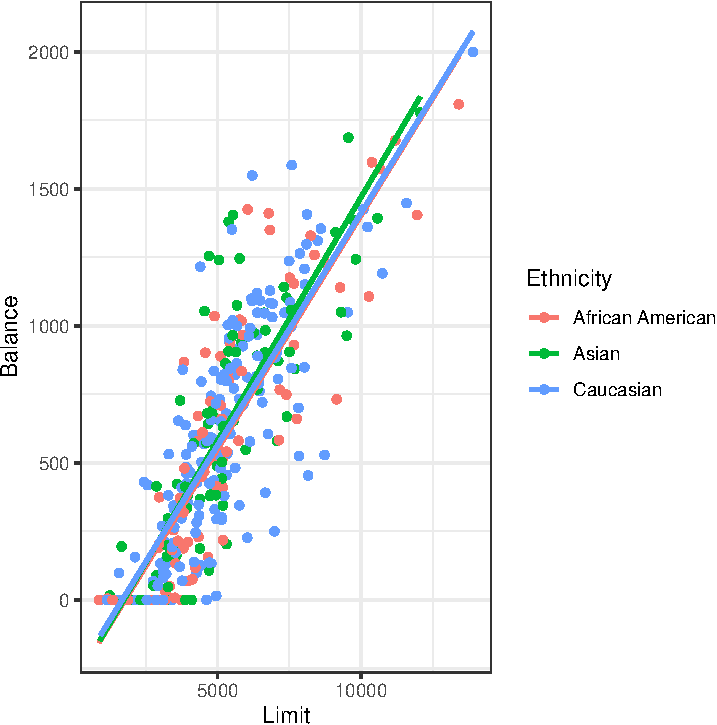
\includegraphics{SDM-CHAP24_files/figure-latex/threesep-1} \end{center}

\textbf{Note:} \texttt{Ethnicity} is not significant, so we really should have just one line.

\begin{Shaded}
\begin{Highlighting}[]
\FunctionTok{ggplot}\NormalTok{(}\AttributeTok{data =}\NormalTok{ Credit, }\FunctionTok{aes}\NormalTok{(}\AttributeTok{x =}\NormalTok{ Limit, }\AttributeTok{y =}\NormalTok{ Balance)) }\SpecialCharTok{+}
  \FunctionTok{geom\_point}\NormalTok{(}\FunctionTok{aes}\NormalTok{(}\AttributeTok{color =}\NormalTok{ Ethnicity)) }\SpecialCharTok{+} 
  \FunctionTok{theme\_bw}\NormalTok{() }\SpecialCharTok{+}
  \FunctionTok{stat\_smooth}\NormalTok{(}\AttributeTok{method =} \StringTok{"lm"}\NormalTok{)}
\end{Highlighting}
\end{Shaded}

\begin{center}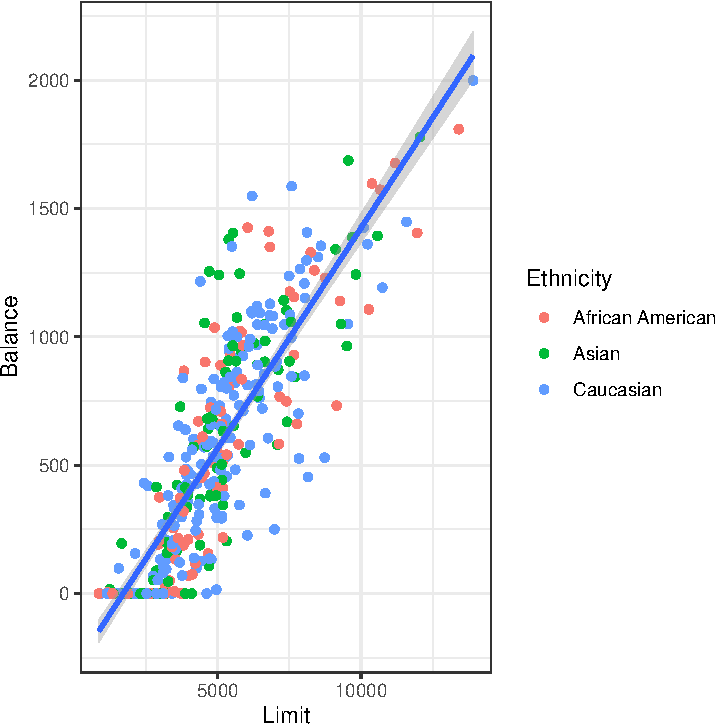
\includegraphics{SDM-CHAP24_files/figure-latex/oneline-1} \end{center}

\hypertarget{matrix-scatterplots}{%
\subsection{Matrix Scatterplots}\label{matrix-scatterplots}}

\begin{Shaded}
\begin{Highlighting}[]
\FunctionTok{scatterplotMatrix}\NormalTok{(}\SpecialCharTok{\textasciitilde{}}\NormalTok{ Balance }\SpecialCharTok{+}\NormalTok{ Income }\SpecialCharTok{+}\NormalTok{ Limit }\SpecialCharTok{+}\NormalTok{ Rating }\SpecialCharTok{+}\NormalTok{ Cards }\SpecialCharTok{+}\NormalTok{ Age }\SpecialCharTok{+}\NormalTok{ Education }\SpecialCharTok{+}\NormalTok{ Gender }\SpecialCharTok{+}\NormalTok{ Student }\SpecialCharTok{+}\NormalTok{ Married }\SpecialCharTok{+}\NormalTok{ Ethnicity,  }\AttributeTok{data =}\NormalTok{ Credit)}
\end{Highlighting}
\end{Shaded}

\begin{center}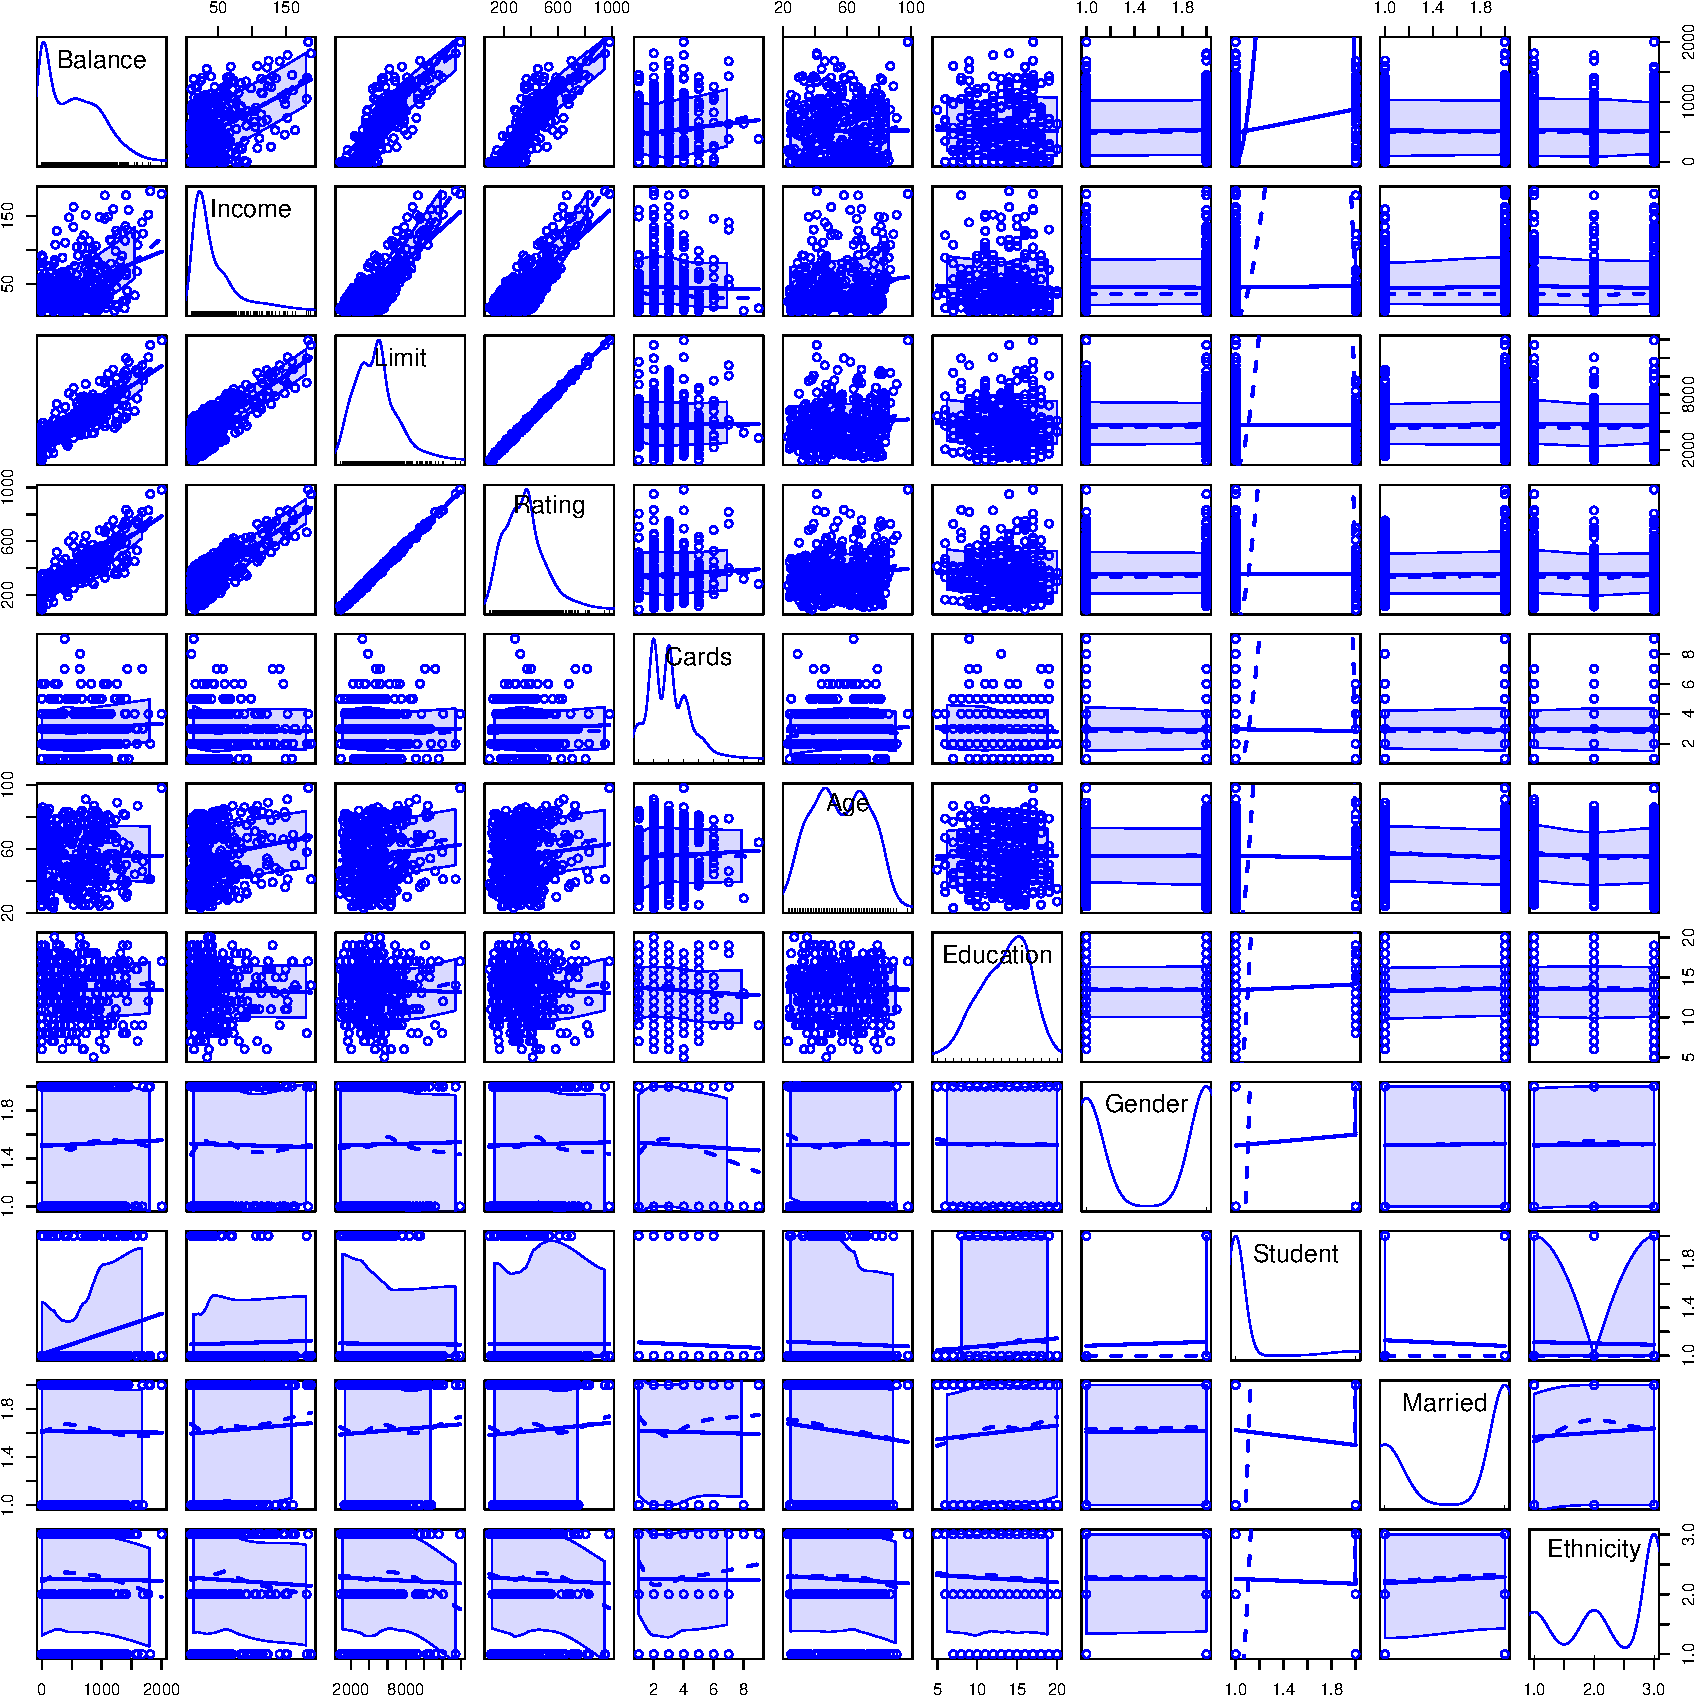
\includegraphics{SDM-CHAP24_files/figure-latex/SP23-1} \end{center}

\begin{Shaded}
\begin{Highlighting}[]
\NormalTok{null }\OtherTok{\textless{}{-}} \FunctionTok{lm}\NormalTok{(Balance }\SpecialCharTok{\textasciitilde{}} \DecValTok{1}\NormalTok{, }\AttributeTok{data =}\NormalTok{ Credit)}
\NormalTok{full }\OtherTok{\textless{}{-}} \FunctionTok{lm}\NormalTok{(Balance }\SpecialCharTok{\textasciitilde{}}\NormalTok{ ., }\AttributeTok{data =}\NormalTok{ Credit)}
\NormalTok{modC }\OtherTok{\textless{}{-}} \FunctionTok{stepAIC}\NormalTok{(full, }\AttributeTok{scope =} \FunctionTok{list}\NormalTok{(}\AttributeTok{lower =}\NormalTok{ null, }\AttributeTok{upper =}\NormalTok{ full), }\AttributeTok{direction =} \StringTok{"backward"}\NormalTok{, }\AttributeTok{test =} \StringTok{"F"}\NormalTok{)}
\end{Highlighting}
\end{Shaded}

\begin{verbatim}
Start:  AIC=3682.12
Balance ~ ID + Income + Limit + Rating + Cards + Age + Education + 
    Gender + Student + Married + Ethnicity + Utilization

              Df Sum of Sq     RSS    AIC F Value     Pr(F)    
- Ethnicity    2     11141 3721961 3679.3    0.58 0.5607055    
- Education    1      2980 3713800 3680.4    0.31 0.5780258    
- ID           1      6003 3716824 3680.8    0.62 0.4298721    
- Gender       1      7246 3718066 3680.9    0.75 0.3858391    
- Married      1      8652 3719472 3681.1    0.90 0.3433763    
<none>                     3710820 3682.1                      
- Age          1     36685 3747505 3684.1    3.82 0.0514884 .  
- Rating       1     51096 3761916 3685.6    5.32 0.0216718 *  
- Utilization  1     67189 3778009 3687.3    6.99 0.0085356 ** 
- Cards        1    130397 3841217 3693.9   13.56 0.0002635 ***
- Limit        1    286876 3997696 3709.9   29.84 8.421e-08 ***
- Income       1   3051935 6762756 3920.2  317.46 < 2.2e-16 ***
- Student      1   4655076 8365896 4005.3  484.22 < 2.2e-16 ***
---
Signif. codes:  0 '***' 0.001 '**' 0.01 '*' 0.05 '.' 0.1 ' ' 1

Step:  AIC=3679.32
Balance ~ ID + Income + Limit + Rating + Cards + Age + Education + 
    Gender + Student + Married + Utilization

              Df Sum of Sq     RSS    AIC F Value     Pr(F)    
- Education    1      3018 3724978 3677.6    0.31 0.5752095    
- ID           1      6005 3727965 3678.0    0.63 0.4293237    
- Married      1      6550 3728511 3678.0    0.68 0.4091349    
- Gender       1      6838 3728799 3678.1    0.71 0.3990231    
<none>                     3721961 3679.3                      
- Age          1     39096 3761056 3681.5    4.08 0.0441954 *  
- Rating       1     48423 3770384 3682.5    5.05 0.0252167 *  
- Utilization  1     70020 3791981 3684.8    7.30 0.0072007 ** 
- Cards        1    133187 3855148 3691.4   13.88 0.0002233 ***
- Limit        1    293994 4015955 3707.7   30.65 5.709e-08 ***
- Income       1   3042199 6764160 3916.3  317.14 < 2.2e-16 ***
- Student      1   4672671 8394632 4002.7  487.11 < 2.2e-16 ***
---
Signif. codes:  0 '***' 0.001 '**' 0.01 '*' 0.05 '.' 0.1 ' ' 1

Step:  AIC=3677.64
Balance ~ ID + Income + Limit + Rating + Cards + Age + Gender + 
    Student + Married + Utilization

              Df Sum of Sq     RSS    AIC F Value     Pr(F)    
- ID           1      6006 3730984 3676.3    0.63 0.4288762    
- Gender       1      6717 3731695 3676.4    0.70 0.4028206    
- Married      1      7188 3732166 3676.4    0.75 0.3868054    
<none>                     3724978 3677.6                      
- Age          1     39443 3764421 3679.9    4.12 0.0430840 *  
- Rating       1     50628 3775606 3681.0    5.29 0.0220135 *  
- Utilization  1     71717 3796695 3683.3    7.49 0.0064909 ** 
- Cards        1    132836 3857815 3689.7   13.87 0.0002246 ***
- Limit        1    291061 4016040 3705.7   30.40 6.431e-08 ***
- Income       1   3040558 6765536 3914.4  317.53 < 2.2e-16 ***
- Student      1   4693948 8418927 4001.8  490.19 < 2.2e-16 ***
---
Signif. codes:  0 '***' 0.001 '**' 0.01 '*' 0.05 '.' 0.1 ' ' 1

Step:  AIC=3676.29
Balance ~ Income + Limit + Rating + Cards + Age + Gender + Student + 
    Married + Utilization

              Df Sum of Sq     RSS    AIC F Value     Pr(F)    
- Married      1      6896 3737880 3675.0    0.72 0.3963978    
- Gender       1      8373 3739357 3675.2    0.88 0.3500974    
<none>                     3730984 3676.3                      
- Age          1     37726 3768710 3678.3    3.94 0.0477529 *  
- Rating       1     50282 3781266 3679.6    5.26 0.0224028 *  
- Utilization  1     74587 3805572 3682.2    7.80 0.0054920 ** 
- Cards        1    130839 3861823 3688.1   13.68 0.0002483 ***
- Limit        1    291132 4022117 3704.3   30.43  6.31e-08 ***
- Income       1   3035245 6766229 3912.4  317.27 < 2.2e-16 ***
- Student      1   4689629 8420613 3999.9  490.21 < 2.2e-16 ***
---
Signif. codes:  0 '***' 0.001 '**' 0.01 '*' 0.05 '.' 0.1 ' ' 1

Step:  AIC=3675.03
Balance ~ Income + Limit + Rating + Cards + Age + Gender + Student + 
    Utilization

              Df Sum of Sq     RSS    AIC F Value     Pr(F)    
- Gender       1      8668 3746548 3674.0    0.91 0.3415625    
<none>                     3737880 3675.0                      
- Age          1     35395 3773275 3676.8    3.70 0.0550578 .  
- Rating       1     47158 3785038 3678.0    4.93 0.0269210 *  
- Utilization  1     72879 3810759 3680.7    7.62 0.0060328 ** 
- Cards        1    135372 3873252 3687.3   14.16 0.0001936 ***
- Limit        1    303600 4041480 3704.3   31.76 3.347e-08 ***
- Income       1   3056864 6794744 3912.1  319.76 < 2.2e-16 ***
- Student      1   4770749 8508629 4002.1  499.04 < 2.2e-16 ***
---
Signif. codes:  0 '***' 0.001 '**' 0.01 '*' 0.05 '.' 0.1 ' ' 1

Step:  AIC=3673.95
Balance ~ Income + Limit + Rating + Cards + Age + Student + Utilization

              Df Sum of Sq     RSS    AIC F Value     Pr(F)    
<none>                     3746548 3674.0                      
- Age          1     35671 3782220 3675.7    3.73 0.0540906 .  
- Rating       1     46902 3793451 3676.9    4.91 0.0273163 *  
- Utilization  1     75071 3821620 3679.9    7.85 0.0053206 ** 
- Cards        1    136510 3883058 3686.3   14.28 0.0001817 ***
- Limit        1    303278 4049826 3703.1   31.73 3.383e-08 ***
- Income       1   3048196 6794744 3910.1  318.93 < 2.2e-16 ***
- Student      1   4765085 8511634 4000.2  498.57 < 2.2e-16 ***
---
Signif. codes:  0 '***' 0.001 '**' 0.01 '*' 0.05 '.' 0.1 ' ' 1
\end{verbatim}

\begin{Shaded}
\begin{Highlighting}[]
\NormalTok{modC}
\end{Highlighting}
\end{Shaded}

\begin{verbatim}
Call:
lm(formula = Balance ~ Income + Limit + Rating + Cards + Age + 
    Student + Utilization, data = Credit)

Coefficients:
(Intercept)       Income        Limit       Rating        Cards          Age  
  -487.7563      -6.9234       0.1823       1.0649      16.3703      -0.5606  
 StudentYes  Utilization  
   403.9969     145.4632  
\end{verbatim}

\begin{Shaded}
\begin{Highlighting}[]
\NormalTok{modD }\OtherTok{\textless{}{-}} \FunctionTok{stepAIC}\NormalTok{(null, }\AttributeTok{scope =} \FunctionTok{list}\NormalTok{(}\AttributeTok{lower =}\NormalTok{ null, }\AttributeTok{upper =}\NormalTok{ full), }\AttributeTok{direction =} \StringTok{"forward"}\NormalTok{, }\AttributeTok{test =} \StringTok{"F"}\NormalTok{)}
\end{Highlighting}
\end{Shaded}

\begin{verbatim}
Start:  AIC=4905.56
Balance ~ 1

              Df Sum of Sq      RSS    AIC F Value     Pr(F)    
+ Rating       1  62904790 21435122 4359.6 1167.99 < 2.2e-16 ***
+ Limit        1  62624255 21715657 4364.8 1147.76 < 2.2e-16 ***
+ Utilization  1  27382381 56957530 4750.5  191.34 < 2.2e-16 ***
+ Income       1  18131167 66208745 4810.7  108.99 < 2.2e-16 ***
+ Student      1   5658372 78681540 4879.8   28.62 1.488e-07 ***
+ Cards        1    630416 83709496 4904.6    3.00   0.08418 .  
<none>                     84339912 4905.6                      
+ Gender       1     38892 84301020 4907.4    0.18   0.66852    
+ Education    1      5481 84334431 4907.5    0.03   0.87231    
+ ID           1      3101 84336810 4907.5    0.01   0.90377    
+ Married      1      2715 84337197 4907.5    0.01   0.90994    
+ Age          1       284 84339628 4907.6    0.00   0.97081    
+ Ethnicity    2     18454 84321458 4909.5    0.04   0.95749    
---
Signif. codes:  0 '***' 0.001 '**' 0.01 '*' 0.05 '.' 0.1 ' ' 1

Step:  AIC=4359.63
Balance ~ Rating

              Df Sum of Sq      RSS    AIC F Value     Pr(F)    
+ Utilization  1  11779424  9655698 4042.6  484.32 < 2.2e-16 ***
+ Income       1  10902581 10532541 4077.4  410.95 < 2.2e-16 ***
+ Student      1   5735163 15699959 4237.1  145.02 < 2.2e-16 ***
+ Age          1    649110 20786012 4349.3   12.40 0.0004798 ***
+ Cards        1    138580 21296542 4359.0    2.58 0.1087889    
+ Married      1    118209 21316913 4359.4    2.20 0.1386707    
<none>                     21435122 4359.6                      
+ Education    1     27243 21407879 4361.1    0.51 0.4776403    
+ Gender       1     16065 21419057 4361.3    0.30 0.5855899    
+ ID           1     14092 21421030 4361.4    0.26 0.6096002    
+ Limit        1      7960 21427162 4361.5    0.15 0.7011619    
+ Ethnicity    2     51100 21384022 4362.7    0.47 0.6233922    
---
Signif. codes:  0 '***' 0.001 '**' 0.01 '*' 0.05 '.' 0.1 ' ' 1

Step:  AIC=4042.64
Balance ~ Rating + Utilization

            Df Sum of Sq     RSS    AIC F Value     Pr(F)    
+ Student    1   2671767 6983931 3915.1 151.493 < 2.2e-16 ***
+ Income     1   1025771 8629927 3999.7  47.069  2.65e-11 ***
+ Married    1     95060 9560638 4040.7   3.937   0.04791 *  
+ Age        1     50502 9605197 4042.5   2.082   0.14983    
<none>                   9655698 4042.6                      
+ Limit      1     42855 9612843 4042.9   1.765   0.18472    
+ Education  1     28909 9626789 4043.4   1.189   0.27616    
+ ID         1     12426 9643273 4044.1   0.510   0.47545    
+ Gender     1      7187 9648511 4044.3   0.295   0.58735    
+ Cards      1      3371 9652327 4044.5   0.138   0.71017    
+ Ethnicity  2     13259 9642439 4046.1   0.272   0.76231    
---
Signif. codes:  0 '***' 0.001 '**' 0.01 '*' 0.05 '.' 0.1 ' ' 1

Step:  AIC=3915.06
Balance ~ Rating + Utilization + Student

            Df Sum of Sq     RSS    AIC F Value   Pr(F)    
+ Income     1   2893712 4090219 3703.1 279.451 < 2e-16 ***
+ Limit      1     77766 6906165 3912.6   4.448 0.03557 *  
+ Age        1     58618 6925313 3913.7   3.343 0.06823 .  
<none>                   6983931 3915.1                    
+ Married    1     33686 6950245 3915.1   1.914 0.16725    
+ Education  1      2344 6981587 3916.9   0.133 0.71591    
+ ID         1      1986 6981946 3916.9   0.112 0.73768    
+ Cards      1      1302 6982630 3917.0   0.074 0.78627    
+ Gender     1         9 6983922 3917.1   0.001 0.98212    
+ Ethnicity  2      1715 6982217 3919.0   0.048 0.95278    
---
Signif. codes:  0 '***' 0.001 '**' 0.01 '*' 0.05 '.' 0.1 ' ' 1

Step:  AIC=3703.06
Balance ~ Rating + Utilization + Student + Income

            Df Sum of Sq     RSS    AIC F Value     Pr(F)    
+ Limit      1    178086 3912133 3687.3 17.9354 2.847e-05 ***
+ Age        1     34096 4056122 3701.7  3.3120   0.06953 .  
<none>                   4090219 3703.1                      
+ Married    1     15941 4074278 3703.5  1.5416   0.21512    
+ Gender     1      8880 4081339 3704.2  0.8572   0.35508    
+ ID         1      5005 4085214 3704.6  0.4827   0.48760    
+ Cards      1      4628 4085591 3704.6  0.4463   0.50447    
+ Education  1       445 4089774 3705.0  0.0428   0.83613    
+ Ethnicity  2     16108 4074111 3705.5  0.7769   0.46054    
---
Signif. codes:  0 '***' 0.001 '**' 0.01 '*' 0.05 '.' 0.1 ' ' 1

Step:  AIC=3687.25
Balance ~ Rating + Utilization + Student + Income + Limit

            Df Sum of Sq     RSS    AIC F Value     Pr(F)    
+ Cards      1    129913 3782220 3675.7 13.4989 0.0002718 ***
+ Age        1     29075 3883058 3686.3  2.9427 0.0870572 .  
<none>                   3912133 3687.3                      
+ Gender     1     10045 3902089 3688.2  1.0116 0.3151296    
+ Married    1      8872 3903262 3688.3  0.8932 0.3451820    
+ ID         1      3818 3908316 3688.9  0.3839 0.5358946    
+ Education  1      3501 3908633 3688.9  0.3520 0.5533444    
+ Ethnicity  2     12590 3899543 3690.0  0.6328 0.5316436    
---
Signif. codes:  0 '***' 0.001 '**' 0.01 '*' 0.05 '.' 0.1 ' ' 1

Step:  AIC=3675.74
Balance ~ Rating + Utilization + Student + Income + Limit + Cards

            Df Sum of Sq     RSS    AIC F Value   Pr(F)  
+ Age        1     35671 3746548 3674.0  3.7323 0.05409 .
<none>                   3782220 3675.7                  
+ Gender     1      8945 3773275 3676.8  0.9293 0.33564  
+ ID         1      5574 3776646 3677.2  0.5785 0.44735  
+ Married    1      4801 3777419 3677.2  0.4982 0.48069  
+ Education  1      3733 3778487 3677.3  0.3873 0.53408  
+ Ethnicity  2     10981 3771239 3678.6  0.5693 0.56641  
---
Signif. codes:  0 '***' 0.001 '**' 0.01 '*' 0.05 '.' 0.1 ' ' 1

Step:  AIC=3673.95
Balance ~ Rating + Utilization + Student + Income + Limit + Cards + 
    Age

            Df Sum of Sq     RSS    AIC F Value  Pr(F)
<none>                   3746548 3674.0               
+ Gender     1    8668.5 3737880 3675.0 0.90676 0.3416
+ ID         1    7358.8 3739190 3675.2 0.76949 0.3809
+ Married    1    7191.5 3739357 3675.2 0.75197 0.3864
+ Education  1    3505.2 3743043 3675.6 0.36616 0.5455
+ Ethnicity  2    8615.0 3737933 3677.0 0.44943 0.6383
\end{verbatim}

\begin{Shaded}
\begin{Highlighting}[]
\NormalTok{modD}
\end{Highlighting}
\end{Shaded}

\begin{verbatim}
Call:
lm(formula = Balance ~ Rating + Utilization + Student + Income + 
    Limit + Cards + Age, data = Credit)

Coefficients:
(Intercept)       Rating  Utilization   StudentYes       Income        Limit  
  -487.7563       1.0649     145.4632     403.9969      -6.9234       0.1823  
      Cards          Age  
    16.3703      -0.5606  
\end{verbatim}

\begin{Shaded}
\begin{Highlighting}[]
\CommentTok{\# Predict}
\FunctionTok{predict}\NormalTok{(modC, }\AttributeTok{newdata =} \FunctionTok{data.frame}\NormalTok{(}\AttributeTok{Income =} \DecValTok{80}\NormalTok{, }\AttributeTok{Limit =} \DecValTok{5000}\NormalTok{, }\AttributeTok{Cards =} \DecValTok{3}\NormalTok{, }\AttributeTok{Age =} \DecValTok{52}\NormalTok{, }\AttributeTok{Student =} \StringTok{"No"}\NormalTok{, }\AttributeTok{Rating =} \DecValTok{800}\NormalTok{, }\AttributeTok{Utilization =} \FloatTok{0.10}\NormalTok{), }\AttributeTok{interval =} \StringTok{"pred"}\NormalTok{)}
\end{Highlighting}
\end{Shaded}

\begin{verbatim}
       fit      lwr      upr
1 756.2699 309.4089 1203.131
\end{verbatim}

\hypertarget{more-diagnostic-plots}{%
\subsection{More Diagnostic Plots}\label{more-diagnostic-plots}}

\begin{Shaded}
\begin{Highlighting}[]
\FunctionTok{residualPlots}\NormalTok{(modC)}
\end{Highlighting}
\end{Shaded}

\begin{center}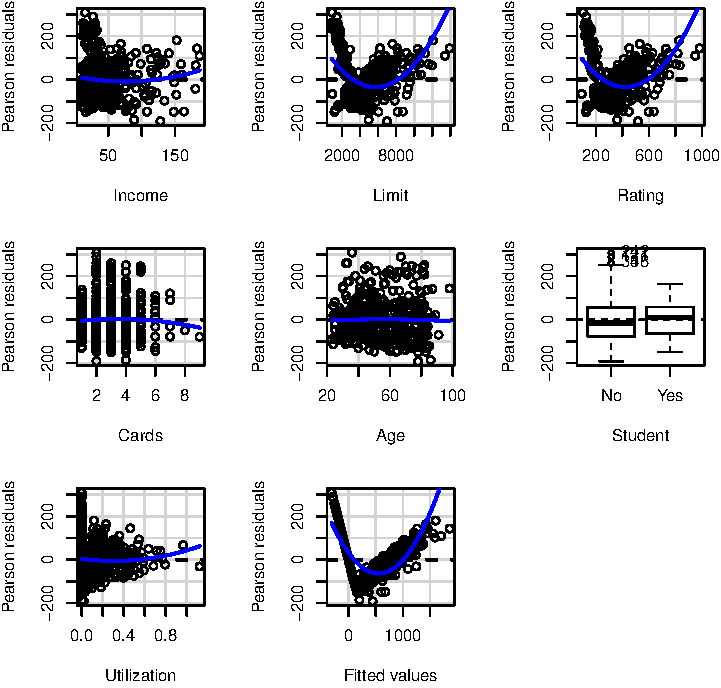
\includegraphics{SDM-CHAP24_files/figure-latex/DPcar-1} \end{center}

\begin{verbatim}
            Test stat Pr(>|Test stat|)    
Income         1.5431           0.1236    
Limit         12.2615           <2e-16 ***
Rating        11.7689           <2e-16 ***
Cards         -0.7709           0.4412    
Age           -0.2795           0.7800    
Student                                   
Utilization    1.4250           0.1550    
Tukey test    25.9407           <2e-16 ***
---
Signif. codes:  0 '***' 0.001 '**' 0.01 '*' 0.05 '.' 0.1 ' ' 1
\end{verbatim}

\begin{Shaded}
\begin{Highlighting}[]
\FunctionTok{qqPlot}\NormalTok{(modC)}
\end{Highlighting}
\end{Shaded}

\begin{center}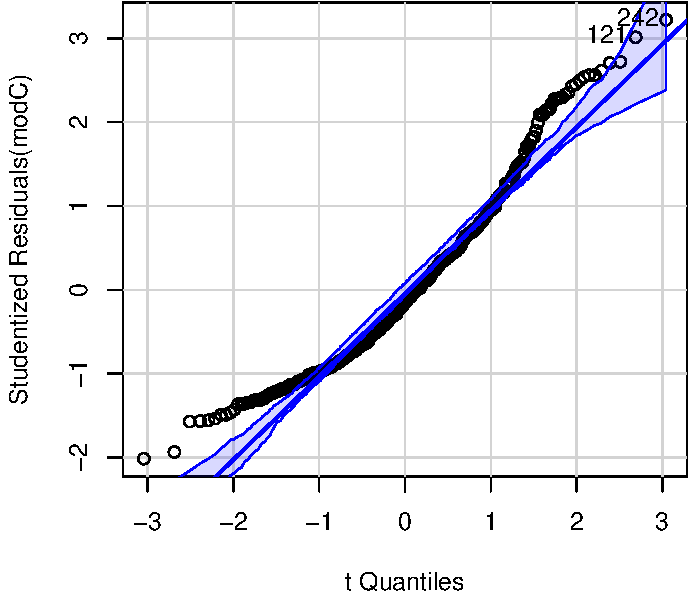
\includegraphics{SDM-CHAP24_files/figure-latex/DPcar-2} \end{center}

\begin{verbatim}
[1] 121 242
\end{verbatim}

\begin{Shaded}
\begin{Highlighting}[]
\FunctionTok{influenceIndexPlot}\NormalTok{(modC)}
\end{Highlighting}
\end{Shaded}

\begin{center}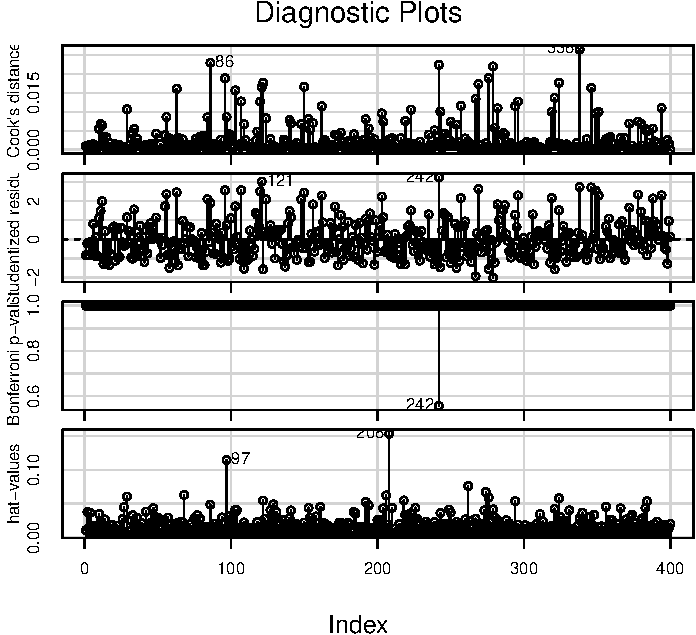
\includegraphics{SDM-CHAP24_files/figure-latex/DPcar-3} \end{center}

\hypertarget{non-linear-relationships}{%
\subsection{Non-linear Relationships}\label{non-linear-relationships}}

\begin{Shaded}
\begin{Highlighting}[]
\FunctionTok{library}\NormalTok{(ISLR)}
\NormalTok{car1 }\OtherTok{\textless{}{-}} \FunctionTok{lm}\NormalTok{(mpg }\SpecialCharTok{\textasciitilde{}}\NormalTok{ horsepower, }\AttributeTok{data =}\NormalTok{ Auto)}
\NormalTok{car2 }\OtherTok{\textless{}{-}} \FunctionTok{lm}\NormalTok{(mpg }\SpecialCharTok{\textasciitilde{}} \FunctionTok{poly}\NormalTok{(horsepower, }\DecValTok{2}\NormalTok{), }\AttributeTok{data =}\NormalTok{ Auto)}
\NormalTok{car5 }\OtherTok{\textless{}{-}} \FunctionTok{lm}\NormalTok{(mpg }\SpecialCharTok{\textasciitilde{}} \FunctionTok{poly}\NormalTok{(horsepower, }\DecValTok{5}\NormalTok{), }\AttributeTok{data =}\NormalTok{ Auto)}
\NormalTok{xs }\OtherTok{\textless{}{-}} \FunctionTok{seq}\NormalTok{(}\FunctionTok{min}\NormalTok{(Auto}\SpecialCharTok{$}\NormalTok{horsepower), }\FunctionTok{max}\NormalTok{(Auto}\SpecialCharTok{$}\NormalTok{horsepower), }\AttributeTok{length =} \DecValTok{500}\NormalTok{)}
\NormalTok{y1 }\OtherTok{\textless{}{-}} \FunctionTok{predict}\NormalTok{(car1, }\AttributeTok{newdata =} \FunctionTok{data.frame}\NormalTok{(}\AttributeTok{horsepower =}\NormalTok{ xs))}
\NormalTok{y2 }\OtherTok{\textless{}{-}} \FunctionTok{predict}\NormalTok{(car2, }\AttributeTok{newdata =} \FunctionTok{data.frame}\NormalTok{(}\AttributeTok{horsepower =}\NormalTok{ xs))}
\NormalTok{y5 }\OtherTok{\textless{}{-}} \FunctionTok{predict}\NormalTok{(car5, }\AttributeTok{newdata =} \FunctionTok{data.frame}\NormalTok{(}\AttributeTok{horsepower =}\NormalTok{ xs))}
\NormalTok{DF }\OtherTok{\textless{}{-}} \FunctionTok{data.frame}\NormalTok{(}\AttributeTok{x =}\NormalTok{ xs, }\AttributeTok{y1 =}\NormalTok{ y1, }\AttributeTok{y2 =}\NormalTok{ y2, }\AttributeTok{y5 =}\NormalTok{ y5)}
\FunctionTok{ggplot}\NormalTok{(}\AttributeTok{data =}\NormalTok{ Auto, }\FunctionTok{aes}\NormalTok{(}\AttributeTok{x =}\NormalTok{ horsepower, }\AttributeTok{y =}\NormalTok{ mpg)) }\SpecialCharTok{+} 
  \FunctionTok{geom\_point}\NormalTok{() }\SpecialCharTok{+} 
  \FunctionTok{theme\_bw}\NormalTok{() }\SpecialCharTok{+} 
  \FunctionTok{geom\_line}\NormalTok{(}\AttributeTok{data =}\NormalTok{ DF, }\FunctionTok{aes}\NormalTok{(}\AttributeTok{x =}\NormalTok{ x, }\AttributeTok{y =}\NormalTok{ y1), }\AttributeTok{color =} \StringTok{"red"}\NormalTok{) }\SpecialCharTok{+} 
  \FunctionTok{geom\_line}\NormalTok{(}\AttributeTok{data =}\NormalTok{ DF, }\FunctionTok{aes}\NormalTok{(}\AttributeTok{x =}\NormalTok{ x, }\AttributeTok{y =}\NormalTok{ y2), }\AttributeTok{color =} \StringTok{"blue"}\NormalTok{) }\SpecialCharTok{+} 
  \FunctionTok{geom\_line}\NormalTok{(}\AttributeTok{data =}\NormalTok{ DF, }\FunctionTok{aes}\NormalTok{(}\AttributeTok{x =}\NormalTok{ x, }\AttributeTok{y =}\NormalTok{ y5), }\AttributeTok{color =} \StringTok{"green"}\NormalTok{)}
\end{Highlighting}
\end{Shaded}

\begin{figure}

{\centering 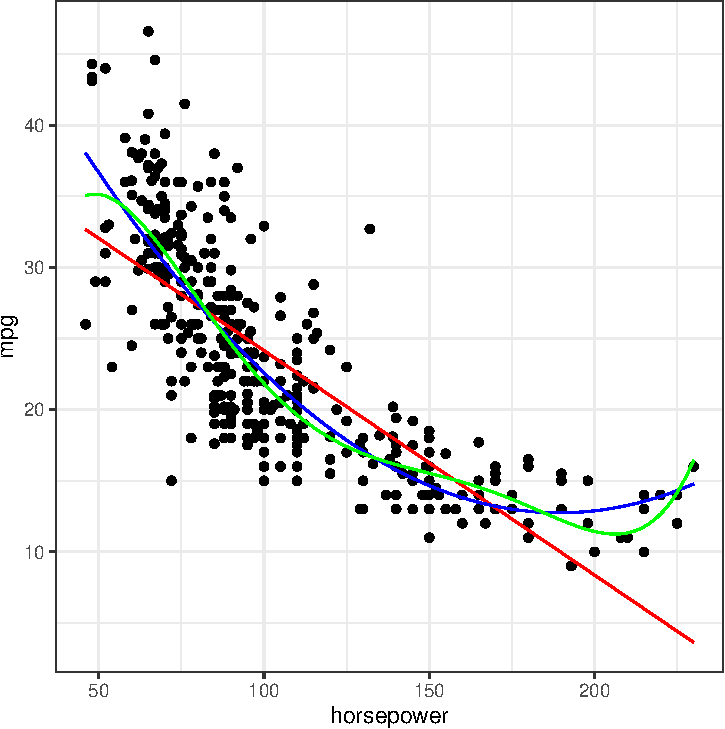
\includegraphics{SDM-CHAP24_files/figure-latex/NLR-1} 

}

\caption{Showing non-linear relationships}\label{fig:NLR}
\end{figure}

\begin{Shaded}
\begin{Highlighting}[]
\FunctionTok{ggplot}\NormalTok{(}\AttributeTok{data =}\NormalTok{ Auto, }\FunctionTok{aes}\NormalTok{(}\AttributeTok{x =}\NormalTok{ horsepower, }\AttributeTok{y =}\NormalTok{ mpg)) }\SpecialCharTok{+} 
  \FunctionTok{geom\_point}\NormalTok{(}\AttributeTok{color =} \StringTok{"lightblue"}\NormalTok{) }\SpecialCharTok{+} 
  \FunctionTok{theme\_bw}\NormalTok{() }\SpecialCharTok{+} 
  \FunctionTok{stat\_smooth}\NormalTok{(}\AttributeTok{method =} \StringTok{"lm"}\NormalTok{, }\AttributeTok{data =}\NormalTok{ Auto, }\AttributeTok{color =} \StringTok{"red"}\NormalTok{, }\AttributeTok{se =} \ConstantTok{FALSE}\NormalTok{) }\SpecialCharTok{+} 
  \FunctionTok{stat\_smooth}\NormalTok{(}\AttributeTok{method =} \StringTok{"lm"}\NormalTok{, }\AttributeTok{formula =}\NormalTok{ y }\SpecialCharTok{\textasciitilde{}} \FunctionTok{poly}\NormalTok{(x, }\DecValTok{2}\NormalTok{), }\AttributeTok{data =}\NormalTok{ Auto, }\AttributeTok{color =} \StringTok{"blue"}\NormalTok{, }\AttributeTok{se =} \ConstantTok{FALSE}\NormalTok{) }\SpecialCharTok{+} 
  \FunctionTok{stat\_smooth}\NormalTok{(}\AttributeTok{method =} \StringTok{"lm"}\NormalTok{, }\AttributeTok{formula =}\NormalTok{ y }\SpecialCharTok{\textasciitilde{}} \FunctionTok{poly}\NormalTok{(x, }\DecValTok{5}\NormalTok{), }\AttributeTok{data =}\NormalTok{ Auto, }\AttributeTok{color =} \StringTok{"green"}\NormalTok{, }\AttributeTok{se =} \ConstantTok{FALSE}\NormalTok{) }
\end{Highlighting}
\end{Shaded}

\begin{center}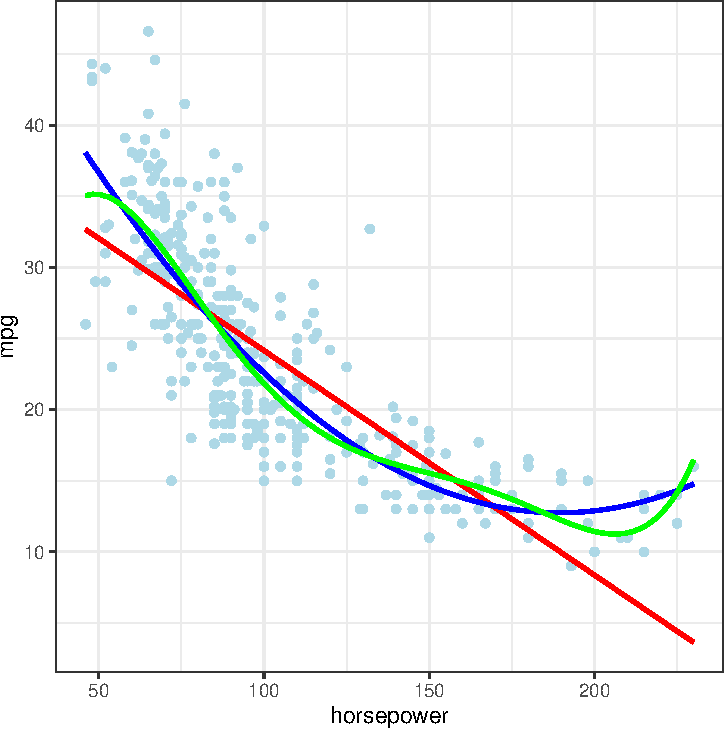
\includegraphics{SDM-CHAP24_files/figure-latex/smooth-1} \end{center}

\begin{Shaded}
\begin{Highlighting}[]
\NormalTok{newC }\OtherTok{\textless{}{-}} \FunctionTok{update}\NormalTok{(modC, .}\SpecialCharTok{\textasciitilde{}}\NormalTok{. }\SpecialCharTok{{-}}\NormalTok{ Limit }\SpecialCharTok{{-}}\NormalTok{ Income }\SpecialCharTok{{-}}\NormalTok{ Rating }\SpecialCharTok{+} \FunctionTok{poly}\NormalTok{(Income, }\DecValTok{2}\NormalTok{) }\SpecialCharTok{+} \FunctionTok{poly}\NormalTok{(Limit, }\DecValTok{4}\NormalTok{))}
\FunctionTok{summary}\NormalTok{(newC)}
\end{Highlighting}
\end{Shaded}

\begin{verbatim}
Call:
lm(formula = Balance ~ Cards + Age + Student + Utilization + 
    poly(Income, 2) + poly(Limit, 4), data = Credit)

Residuals:
    Min      1Q  Median      3Q     Max 
-327.92  -31.35   -3.54   30.91  200.35 

Coefficients:
                   Estimate Std. Error t value Pr(>|t|)    
(Intercept)        408.5875    12.2594  33.328  < 2e-16 ***
Cards               17.2245     2.1497   8.013 1.32e-14 ***
Age                 -0.7256     0.1699  -4.270 2.46e-05 ***
StudentYes         369.4275    10.7980  34.213  < 2e-16 ***
Utilization        422.8552    36.6956  11.523  < 2e-16 ***
poly(Income, 2)1 -5263.1585   167.9209 -31.343  < 2e-16 ***
poly(Income, 2)2  -896.3437    95.2993  -9.406  < 2e-16 ***
poly(Limit, 4)1  11775.8484   165.8389  71.008  < 2e-16 ***
poly(Limit, 4)2   1920.4673    97.7898  19.639  < 2e-16 ***
poly(Limit, 4)3   -814.2430    61.0972 -13.327  < 2e-16 ***
poly(Limit, 4)4    393.7068    59.2827   6.641 1.05e-10 ***
---
Signif. codes:  0 '***' 0.001 '**' 0.01 '*' 0.05 '.' 0.1 ' ' 1

Residual standard error: 57.15 on 389 degrees of freedom
Multiple R-squared:  0.9849,    Adjusted R-squared:  0.9845 
F-statistic:  2544 on 10 and 389 DF,  p-value: < 2.2e-16
\end{verbatim}

\begin{Shaded}
\begin{Highlighting}[]
\FunctionTok{residualPlots}\NormalTok{(newC)}
\end{Highlighting}
\end{Shaded}

\begin{center}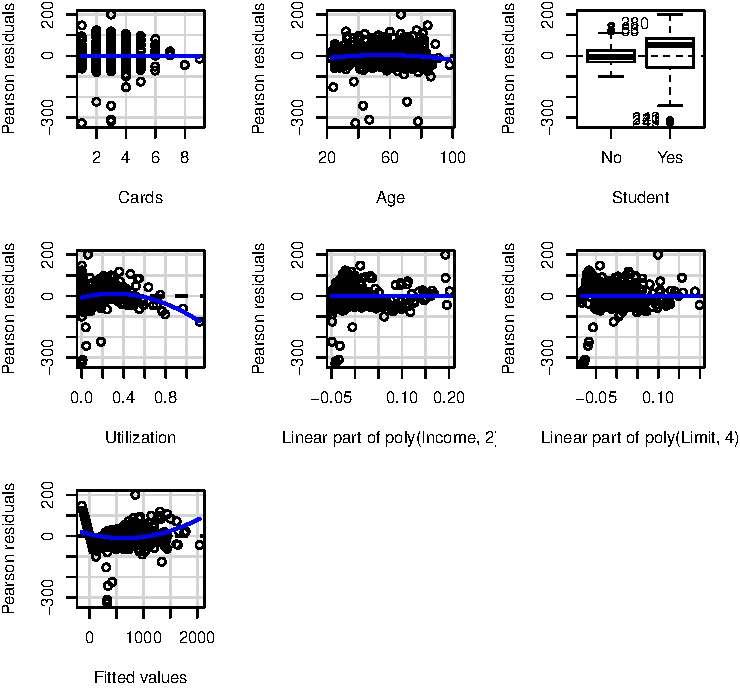
\includegraphics{SDM-CHAP24_files/figure-latex/unnamed-chunk-4-1} \end{center}

\begin{verbatim}
                Test stat Pr(>|Test stat|)    
Cards             -0.1284           0.8979    
Age               -1.2123           0.2261    
Student                                       
Utilization       -5.4273        1.010e-07 ***
poly(Income, 2)                               
poly(Limit, 4)                                
Tukey test         8.1970        2.465e-16 ***
---
Signif. codes:  0 '***' 0.001 '**' 0.01 '*' 0.05 '.' 0.1 ' ' 1
\end{verbatim}

\begin{Shaded}
\begin{Highlighting}[]
\FunctionTok{qqPlot}\NormalTok{(newC)}
\end{Highlighting}
\end{Shaded}

\begin{center}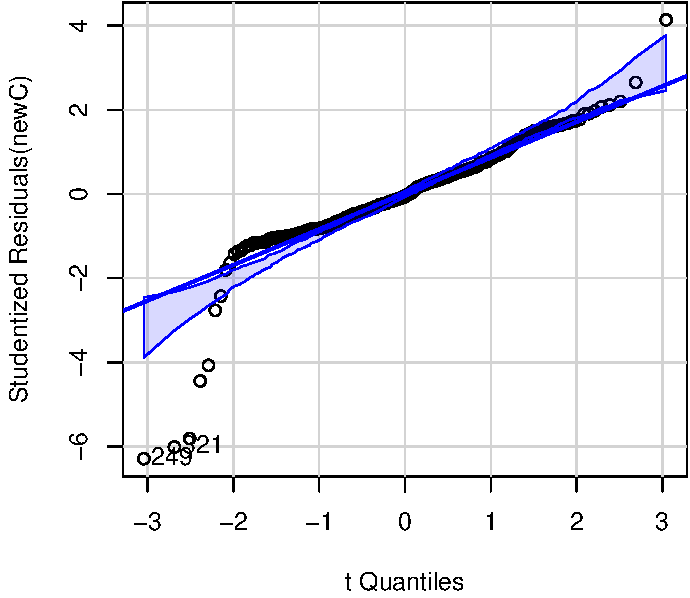
\includegraphics{SDM-CHAP24_files/figure-latex/unnamed-chunk-4-2} \end{center}

\begin{verbatim}
[1] 249 321
\end{verbatim}

\begin{Shaded}
\begin{Highlighting}[]
\FunctionTok{influenceIndexPlot}\NormalTok{(newC)}
\end{Highlighting}
\end{Shaded}

\begin{center}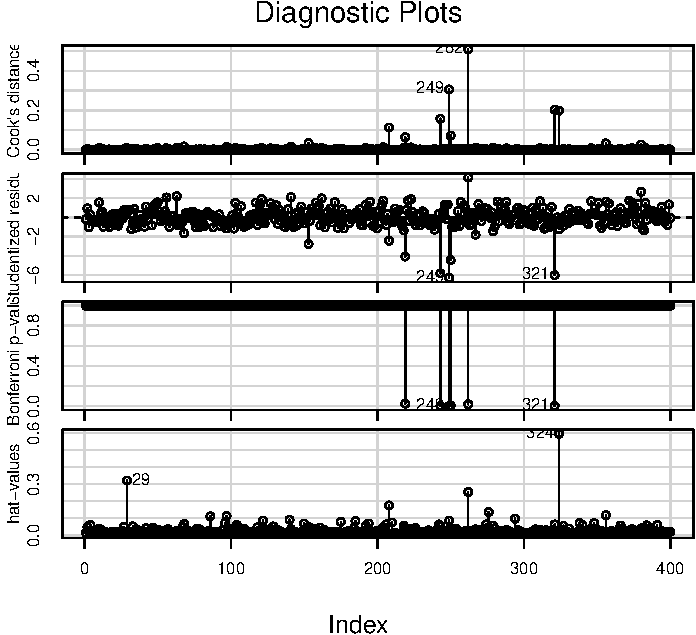
\includegraphics{SDM-CHAP24_files/figure-latex/unnamed-chunk-4-3} \end{center}

\hypertarget{variance-inflation-factor-vif}{%
\subsection{Variance Inflation Factor (VIF)}\label{variance-inflation-factor-vif}}

The VIF is the ratio of the variance of \(\hat{\beta}_j\) when fitting the full model divided by the variance of \(\hat{\beta}_j\) if it is fit on its own. The smallest possible value for VIF is 1, which indicates the complete absence of collinearity. The VIF for each variable can be computed using the formula:

\[VIF(\hat{\beta}_j) = \frac{1}{1 - R^2_{X_j|X_{-j}}}\]

where \(R^2_{X_j|X_{-j}}\) is the \(R^2\) from a regression of \(X_j\) onto all of the other predictors. If \(R^2_{X_j|X_{-j}}\) is close to one, then collinearity is present, and so the VIF will be large.

Compute the VIF for each \(\hat{\beta}_j\) of \texttt{modC}

\begin{Shaded}
\begin{Highlighting}[]
\NormalTok{modC}
\end{Highlighting}
\end{Shaded}

\begin{verbatim}
Call:
lm(formula = Balance ~ Income + Limit + Rating + Cards + Age + 
    Student + Utilization, data = Credit)

Coefficients:
(Intercept)       Income        Limit       Rating        Cards          Age  
  -487.7563      -6.9234       0.1823       1.0649      16.3703      -0.5606  
 StudentYes  Utilization  
   403.9969     145.4632  
\end{verbatim}

\begin{Shaded}
\begin{Highlighting}[]
\NormalTok{R2inc }\OtherTok{\textless{}{-}} \FunctionTok{summary}\NormalTok{(}\FunctionTok{lm}\NormalTok{(Income }\SpecialCharTok{\textasciitilde{}}\NormalTok{ Limit }\SpecialCharTok{+}\NormalTok{ Rating }\SpecialCharTok{+}\NormalTok{ Cards }\SpecialCharTok{+}\NormalTok{ Age }\SpecialCharTok{+}\NormalTok{ Student }\SpecialCharTok{+}\NormalTok{ Utilization, }\AttributeTok{data =}\NormalTok{ Credit))}\SpecialCharTok{$}\NormalTok{r.squared}
\NormalTok{R2inc}
\end{Highlighting}
\end{Shaded}

\begin{verbatim}
[1] 0.8716908
\end{verbatim}

\begin{Shaded}
\begin{Highlighting}[]
\NormalTok{VIFinc }\OtherTok{\textless{}{-}} \DecValTok{1}\SpecialCharTok{/}\NormalTok{(}\DecValTok{1} \SpecialCharTok{{-}}\NormalTok{ R2inc)}
\NormalTok{VIFinc}
\end{Highlighting}
\end{Shaded}

\begin{verbatim}
[1] 7.793671
\end{verbatim}

\begin{Shaded}
\begin{Highlighting}[]
\NormalTok{R2lim }\OtherTok{\textless{}{-}} \FunctionTok{summary}\NormalTok{(}\FunctionTok{lm}\NormalTok{(Limit }\SpecialCharTok{\textasciitilde{}}\NormalTok{ Income }\SpecialCharTok{+}\NormalTok{ Rating }\SpecialCharTok{+}\NormalTok{ Cards }\SpecialCharTok{+}\NormalTok{ Age }\SpecialCharTok{+}\NormalTok{ Student }\SpecialCharTok{+}\NormalTok{ Utilization, }\AttributeTok{data =}\NormalTok{ Credit))}\SpecialCharTok{$}\NormalTok{r.squared}
\NormalTok{R2lim}
\end{Highlighting}
\end{Shaded}

\begin{verbatim}
[1] 0.9957067
\end{verbatim}

\begin{Shaded}
\begin{Highlighting}[]
\NormalTok{VIFlim }\OtherTok{\textless{}{-}} \DecValTok{1}\SpecialCharTok{/}\NormalTok{(}\DecValTok{1} \SpecialCharTok{{-}}\NormalTok{ R2lim)}
\NormalTok{VIFlim}
\end{Highlighting}
\end{Shaded}

\begin{verbatim}
[1] 232.9193
\end{verbatim}

This is tedious is there a function to do this? Yes!

\begin{Shaded}
\begin{Highlighting}[]
\NormalTok{car}\SpecialCharTok{::}\FunctionTok{vif}\NormalTok{(modC)}
\end{Highlighting}
\end{Shaded}

\begin{verbatim}
     Income       Limit      Rating       Cards         Age     Student 
   7.793671  232.919318  230.957276    1.472901    1.046060    1.233070 
Utilization 
   3.323397 
\end{verbatim}

\begin{center}\rule{0.5\linewidth}{0.5pt}\end{center}

\hypertarget{building-models-with-leaps}{%
\subsubsection{\texorpdfstring{Building Models with \texttt{leaps}}{Building Models with leaps}}\label{building-models-with-leaps}}

\begin{Shaded}
\begin{Highlighting}[]
\FunctionTok{library}\NormalTok{(leaps)}
\NormalTok{bestsubsetmodel }\OtherTok{\textless{}{-}} \FunctionTok{regsubsets}\NormalTok{(Balance }\SpecialCharTok{\textasciitilde{}}\NormalTok{ ., }\AttributeTok{data =}\NormalTok{ Credit)}
\FunctionTok{plot}\NormalTok{(bestsubsetmodel, }\AttributeTok{scale =} \StringTok{"Cp"}\NormalTok{)}
\end{Highlighting}
\end{Shaded}

\begin{center}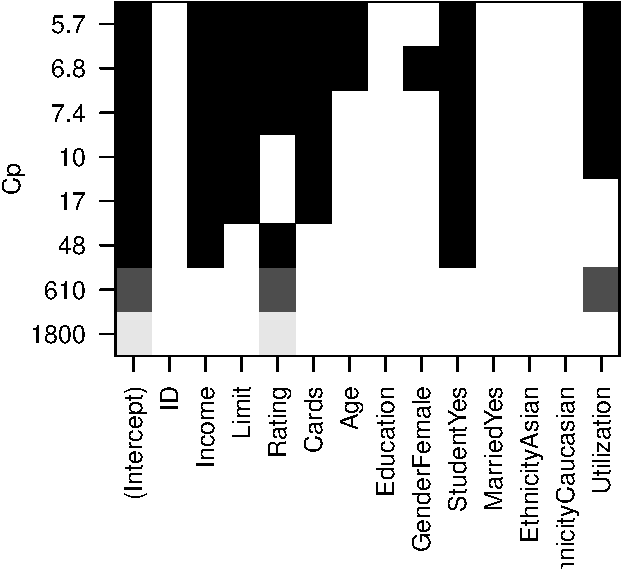
\includegraphics{SDM-CHAP24_files/figure-latex/unnamed-chunk-6-1} \end{center}

\begin{Shaded}
\begin{Highlighting}[]
\FunctionTok{plot}\NormalTok{(bestsubsetmodel, }\AttributeTok{scale =} \StringTok{"adjr2"}\NormalTok{)}
\end{Highlighting}
\end{Shaded}

\begin{center}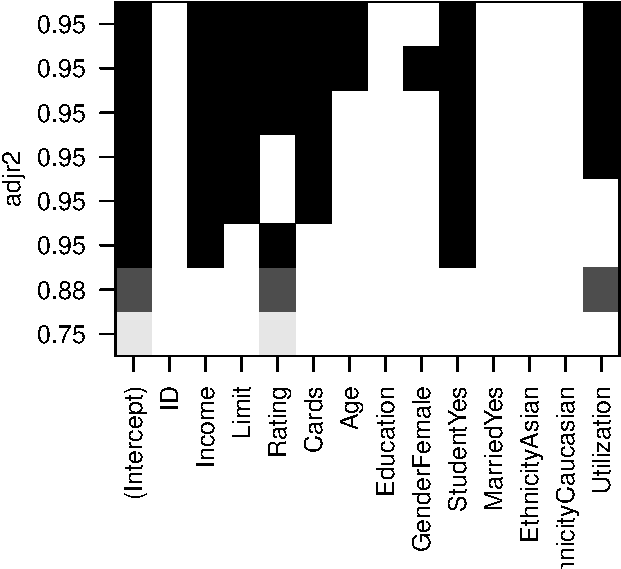
\includegraphics{SDM-CHAP24_files/figure-latex/unnamed-chunk-6-2} \end{center}

\begin{Shaded}
\begin{Highlighting}[]
\FunctionTok{plot}\NormalTok{(bestsubsetmodel, }\AttributeTok{scale =} \StringTok{"r2"}\NormalTok{)}
\end{Highlighting}
\end{Shaded}

\begin{center}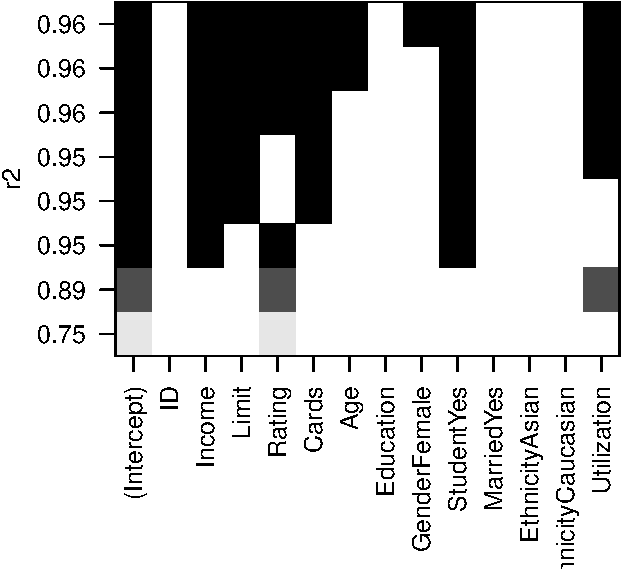
\includegraphics{SDM-CHAP24_files/figure-latex/unnamed-chunk-6-3} \end{center}

\begin{Shaded}
\begin{Highlighting}[]
\FunctionTok{plot}\NormalTok{(bestsubsetmodel, }\AttributeTok{scale =} \StringTok{"bic"}\NormalTok{)}
\end{Highlighting}
\end{Shaded}

\begin{center}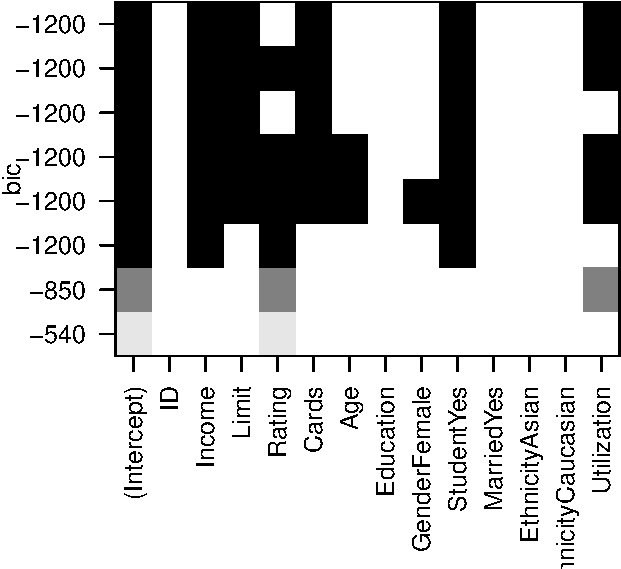
\includegraphics{SDM-CHAP24_files/figure-latex/unnamed-chunk-6-4} \end{center}

\begin{Shaded}
\begin{Highlighting}[]
\FunctionTok{coef}\NormalTok{(bestsubsetmodel, }\DecValTok{7}\NormalTok{)}
\end{Highlighting}
\end{Shaded}

\begin{verbatim}
 (Intercept)       Income        Limit       Rating        Cards          Age 
-487.7563318   -6.9233687    0.1822902    1.0649244   16.3703375   -0.5606190 
  StudentYes  Utilization 
 403.9969037  145.4632091 
\end{verbatim}

\begin{center}\rule{0.5\linewidth}{0.5pt}\end{center}

\hypertarget{exercise}{%
\subsection{Exercise}\label{exercise}}

\begin{itemize}
\item
  Create a model that predicts an individuals credit rating (\texttt{Rating}).
\item
  Create another model that predicts rating with \texttt{Limit}, \texttt{Cards}, \texttt{Married}, \texttt{Student}, and \texttt{Education} as features.
\item
  Use your model to predict the \texttt{Rating} for an individual that has a credit card limit of
  \$6,000, has 4 credit cards, is married, is not a student, and has an undergraduate degree (\texttt{Education} = 16).
\item
  Use your model to predict the \texttt{Rating} for an individual that has a credit card limit of
  \$12,000, has 2 credit cards, is married, is not a student, and has an eighth grade education (\texttt{Education} = 8).
\end{itemize}

\end{document}
